\documentclass{article}
\usepackage[utf8]{inputenc}
\usepackage{amssymb}
\usepackage{amsmath}
\usepackage{tikz}
% \usepackage{algorithm}
% \usepackage{algorithmic}
\usepackage[ruled]{algorithm2e}
\usepackage{graphicx}
\usepackage{fancyhdr}
%\usepackage{biblatex}
\usepackage{url}
\usepackage{float}
%\usepackage{ulem}
\usepackage{parskip}
\usepackage{pdflscape}
\usepackage{svg}
\usepackage{tabularx}
\usepackage{longtable}

%%%%%%% MUST BE LOADED LAST IN THE PACKAGE DOCUMENT! %%%%%%%%%%
\usepackage[hidelinks]{hyperref}
\usepackage[noabbrev]{cleveref}
\newlength\mylen
\newcommand\myinput[1]{%
  \settowidth\mylen{\KwData{}}%
  \setlength\hangindent{\mylen}%
  \hspace*{\mylen}#1\\}

\newcommand\KwMoreData[1]{%
  \settowidth\mylen{\KwData{}}%
  \setlength\hangindent{\mylen}%
  \hspace*{\mylen}#1\\}
  
\SetKw{KwAnd}{and}
\SetKw{KwOr}{or}
\SetKw{KwBy}{by}
\SetKw{KwForEach}{for each}
\SetKw{Continue}{continue}

\renewcommand\arraystretch{1.5}

\makeatletter
\newdimen\multi@col@width
\newdimen\multi@col@margin
\newcount\multi@col@count
\multi@col@width=0pt



% internal node styles
\tikzset{
  block_font/.style = {font=\small},
  banner_font/.style = {font=\scriptsize},
  half_size/.style = {text width=160},
  third_size/.style = {text width=173},
  block_background/.style = {fill=black!5}
}

% main types of nodes
\tikzset{
  title/.style = {half_size, minimum height=20, align=center},
  title_3/.style = {title, third_size},
  ik/.style = {block_font, align=center, anchor=north},
  block/.style = {block_font, align=left, draw, dotted, rounded corners, block_background},
  arrow/.style = {block_font, align=center, anchor=north west},
  banner/.style = {banner_font, align=center}
}

% other helpful node styles
\tikzset{
  spaced/.style={yshift=-7},
  keep_left/.style={anchor=north west},
  keep_middle/.style={anchor=north},
  keep_right/.style={anchor=north east},
  immediate/.style={spaced, anchor=south west},
  towards_right/.style = {append after command={
    [->] (\tikzlastnode.south west)edge(\tikzlastnode.south east)}},
  towards_left/.style = {append after command={
    [->] (\tikzlastnode.south east)edge(\tikzlastnode.south west)}},
  between/.style 2 args={
      insert path={
          \pgfextra{
              \path (#1);
              \pgfgetlastxy{\xa}{\ya} 
              \path (#2);
              \pgfgetlastxy{\xb}{\yb}   
              \pgfpointdiff{\pgfpoint{\xa}{\ya}}{\pgfpoint{\xb}{\yb}}
              \pgf@xa=\pgf@x
          }
      },
      minimum width=\pgf@xa
  }
}

\tikzset{
  multicol/.code={%
    \global\multi@col@count=#1\relax
    \global\let\orig@pgfmatrixendcode=\pgfmatrixendcode
    \global\let\orig@pgfmatrixemptycode=\pgfmatrixemptycode
    \def\pgfmatrixendcode##1{\orig@pgfmatrixendcode%
      ##1%
      \pgfutil@tempdima=\pgf@picmaxx
      \global\multi@col@margin=\pgf@picminx
      \advance\pgfutil@tempdima by -\pgf@picminx
      \divide\pgfutil@tempdima by #1\relax
      \global\multi@col@width=\pgfutil@tempdima
      \pgf@picmaxx=.5\multi@col@width
      \pgf@picminx=-.5\multi@col@width
      \global\pgf@picmaxx=\pgf@picmaxx
      \global\pgf@picminx=\pgf@picminx
  \gdef\multi@adjust@position{%
     \setbox\pgf@matrix@cell=\hbox\bgroup
     \hfil\hskip-1.5\multi@col@margin
     \hfil\hskip-.5\multi@col@width     
% \gdef\multi@adjust@position{%
%        \setbox\pgf@matrix@cell=\hbox\bgroup
%        \hfil\hskip-\multi@col@margin
%        \hfil\hskip-.5\multi@col@width
        \box\pgf@matrix@cell
        \egroup
      }%
      \gdef\multi@temp{\aftergroup\multi@adjust@position}%
      \aftergroup\multi@temp
    }
    \gdef\pgfmatrixemptycode{%
      \orig@pgfmatrixemptycode
      \global\advance\multi@col@count by -1\relax
      \global\pgf@picmaxx=.5\multi@col@width
      \global\pgf@picminx=-.5\multi@col@width
      \ifnum\multi@col@count=1\relax
       \global\let\pgfmatrixemptycode=\orig@pgfmatrixemptycode
      \fi
    }
  }
}
% Set path for graphics for the package 'graphicx'
\graphicspath{ {./Pictures/} }

% Settings for package 'fancyhdr'
\usetikzlibrary{backgrounds, matrix, shapes, arrows, positioning, chains, calc}


\renewcommand{\headrulewidth}{0pt}
\pagestyle{fancy}
\fancyhf{}
%\lhead{\includegraphics[height=0.3in]{av-logo-horizontalw200.png}}
\lhead{
\includegraphics[height=0.3in]{Pictures/1.corporate_logo_blue.png}}
\cfoot{\thepage}
%\renewcommand\maketitle{}

% ENABLE SUBSUBSUB SECTION
%\setcounter{secnumdepth}{5}
%\setcounter{tocdepth}{5}
%\newcommand\subsubsubsection{\@startsection{paragraph}{4}{\z@}{-2.5ex\@plus -1ex \@minus -.25ex}{1.25ex \@plus .25ex}{\normalfont\normalsize\bfseries}}
%\newcommand\subsubsubsubsection{\@startsection{subparagraph}{5}{\z@}{-2.5ex\@plus -1ex \@minus -.25ex}{1.25ex \@plus .25ex}{\normalfont\normalsize\bfseries}}
%

%\fancypagestyle{lscape}{% 
%\fancyhf{} % clear all header and footer fields 
%\fancyfoot[LE]{%
%\begin{textblock}{20}(1,5){\rotatebox{90}{\leftmark}}\end{textblock}
%\begin{textblock}{1}(13,10.5){\rotatebox{90}{\thepage}}\end{textblock}}
%\fancyfoot[LO] {%
%\begin{textblock}{1}(13,10.5){\rotatebox{90}{\thepage}}\end{textblock}
%\begin{textblock}{20}(1,13.25){\rotatebox{90}{\rightmark}}\end{textblock}}
%\renewcommand{\headrulewidth}{0pt} 
%\renewcommand{\footrulewidth}{0pt}}

%%%%% DEFINING COLORS %%%%%%
\definecolor{asparagus}{rgb}{0.53, 0.66, 0.42}
\definecolor{applegreen}{rgb}{0.55, 0.71, 0.0}
\definecolor{darkpastelgreen}{rgb}{0.01, 0.75, 0.24}


\makeatother



\title{AVX}
\author{Assembly Voting}
\date{19 January 2023}

\begin{document}

\maketitle
%\thispagestyle{fancy}
\thispagestyle{empty}

\begin{center}{\large \textbf{Documentation of the cryptographic protocol}} \end{center}
\begin{center} {\large Version x.x} \end{center}

\begin{tikzpicture}[remember picture,overlay]
\node[anchor=south, % anchor is bottom of picture
      xshift=0pt, 
      yshift=-2.9mm] % shifting picture to actually be at the bottom of the page
     at (current page.south) % placement at bottom of the page
     {
\includegraphics[height=18.9cm,width=25cm,keepaspectratio]{Pictures/LinkedIn_Covers2.jpg}};
\end{tikzpicture}

\newpage
\pagenumbering{roman}
\section*{Abstract}
\addcontentsline{toc}{section}{Abstract}
\setlength{\headheight}{25.28125pt}
Contents for abstract is written here

\newpage
\tableofcontents
\newpage

%%%%%%%%%%%%%%%%%%%%%%%%%%%%%%%%%%
\pagenumbering{arabic}
\section{Introduction}

\subsection{State of solution}
This document presents all the technical details of the cryptographic design of the internet voting system, Assembly Voting X (AVX). The system presented is the proposed design of the upcoming version (v. 2.0) of the production system (v. 1.0) currently used in elections throughout the world.

Apart from the core features of the product described in the main sections, the \cref{app: affidavit document extension} section and the \cref{app: multiple result extractions} section present add-on functionality required for the Mobile Voting Project \cite{Tusk} in the US.

\subsection{Intended audience}
The document is primarily intended for cryptographers or technical, mathematical readers. The Threat model in \cref{sec: threat model} covers non-cryptographic, non-mathematical topics and targets readers with more general interests in security in online electoral systems.

\subsection{Protocol scope and objectives}
Some of the core features of the election protocol include: voters vote remotely, votes are encrypted, the system uses threshold cryptography, votes are cryptographically shuffled to ensure anonymity, all essential processes are verifiable, and auditing can be performed on all system components throughout the election event. The system cannot prevent but detects fraud or unauthorized access.

Multiple election types are supported, such as a referendum, candidate, multiple choice, or ranked elections. Multiple result types are also supported. The protocol has support for write-in votes. Additionally, the system provides continuous turnout statistics.

The scope of the protocol covers an entire election event, starting from election configuration, voter authorization, vote casting, tallying, and auditing. Cryptographic algorithms are crucial in terms of the security and auditing features of the system, but there are many non-cryptographic processes necessary to conduct a safe election. This document describes an online election system. Users, i.e., election officials and voters, access the system through a web browser or a native app on an internet-connected device such as a PC, laptop, tablet, smartphone, etc.

The overall objective of the document is to describe, claim and argue the achievement of the following objectives of our protocol, which are described in \cref{sec: requirements}:
\begin{multicols}{2}
\begin{itemize}
    \item Mobility
    \item Vote \& go
    \item Transparency
    \item Multiple voting rounds
    \item Multiple election types
    \item Confirming selected options
    \item Support correcting mistakes
    \item Vote overwrites
    \item Individual verification
    \item Universal verification    
    \item Full audit
    \item Eligibility
    \item Privacy
    \item Anonymity
    \item Integrity
    \item Ent-to-end verifiability
    \item Receipt-freeness.
\end{itemize}
\end{multicols}

\subsection{Document outline}
\Cref{sec: solution entities} lists all the key parts of the election system, including the stakeholders, system components, and the communication channels they use in the protocol. Then, it presents the implications of having a public bulletin board that collects all election data. Next, it describes the voter authentication modes that are supported. The section ends with a list of requirements the election system must fulfill.

\Cref{sec: election protocol} presents the cryptographic algorithms and processes that the election entities must follow in the life cycle of an election. The section is split into pre-election, election, and post-election processes. The section ends by listing the election properties and explaining how they are achieved.

\Cref{sec: auditing} presents all the auditing processes. It describes who can perform each particular audit process, when it can happen, and what inputs are needed.

\Cref{sec: adversary model} presents the adversary model that the system is designed to handle. It lists all trust assumptions the system relies on, the threats arising from them, and how they are mitigated.

\Cref{app: theoretical background} lists the applied cryptographic algorithms and their mathematical principles.

\Cref{app: bulletin board item types} contains a comprehensive list of all items that appear on the public bulletin board. It defines the rules and structure for each item type.

\Cref{app: extra features} presents a list of additional optional features that are not considered as the core product. Each feature is described in terms of how it modifies the election protocol and how it impacts the election properties.

\clearpage
\section{Solution entities} \label{sec:solution entities}
This section describes the different entities seen throughout this documentation in addition to the requirements.

\subsection{Election roles} \label{sec: election roles}
Multiple parties are involved in the election process. Each party represents a human with access to a computer or simply a process/software that follows a particular protocol. All these parties can be categorized into the following 9 types: 


\subsubsection{Election Administrator}
There exists one administrator that is responsible for setting up the election event and making updates to the configurations. The Election Administrator $\mathcal{E}$ is a single service that is used by all election officers to configure the election. Election officers are humans that use an internet connected device to access the Election Administrator service based on some pre-established set of credentials.

The Election Administrator $\mathcal{E}$ owns a key pair $(x_\mathcal{E}, Y_\mathcal{E})$ used for signing the election configuration and it is responsible for privately storing its private key $x_\mathcal{E}$.


\subsubsection{Voter}
There exists a list of eligible voters, each denoted $\mathcal{V}_i$, with \( i \in \{ 1, ..., n_\mathrm{v} \} \), where $n_\mathrm{v}$ is the total number of voters.  A voter is a human being that is allowed to cast a valid vote in this election. A voter needs to have access to a computer that has an internet connection. Voters are the ones to generate vote cryptograms.

In \textit{pre-election} voter registration mode (see \cref{sec: voter registration modes}), voters are responsible for protecting their credentials $x_{i,j}$ received from all printing authorities or the single credential in the case that only one printing authority is used.

In \textit{on-demand} voter registration mode voters are responsible for protecting their private key $x_i$ while a voting session is active.


\subsubsection{Printing Authority}
The Printing Authority role is relevant only in the \textit{pre-election} voter registration mode, which is described in \cref{sec: pre-election mode}.
    
There is a set of printing authorities, each noted as $\mathcal{P}_i$, with \( i \in \{ 1, ..., n_\mathrm{p} \} \), where $n_\mathrm{p}$ is the total number of printing authorities. A printing authority is an institution, consisting of humans and software processes. Each of them is responsible for generating voter credentials and distribute them privately to the voters. It is recommended that each printing authority should use a different communication channel for distributing credentials (e.g. e-mail, post, SMS). Printing Authorities must delete the voter credentials after they have been distributed.


\subsubsection{Trustee}
There is a set of trustees, each denoted as $\mathcal{T}_i$, with \( i \in \{ 1, ..., n_\mathrm{t} \} \), where $n_\mathrm{t}$ is the total number of trustees. A trustee is a human controlling a computer that has the \textit{Trustee Application} installed. Trustees are responsible for preserving the privacy and the fairness of the election during the election phase by working together to build the election encryption key while safely storing their shares of the decryption key.

The Trustee $\mathcal{T}_i$ protects its own private key $x_{\mathcal{T}_i}$ and its share of the election decryption key $sx_i$.

Trustees are also responsible for preserving the anonymity of the election by shuffling the entire list of votes in an indistinguishable way before a result is computed.


\subsubsection{Identity Provider}
The Identity Provider role is relevant only in the \textit{on-demand} voter registration mode, which is described in \cref{sec: on-demand mode}.
    
There is a set of Identity Providers $\mathcal{I}_i$, with $i \in \{ 1, ..., n_\mathrm{i} \}$, where $n_\mathrm{i}$ is the total number of identity providers. An Identity Provider is a third party application responsible for authenticating a voter $\mathcal{V}$, on the fly, during the election phase. Identity Providers must follow the OIDC protocol.


\subsubsection{Voter Authorizer} 
The Voter Authorizer $\mathcal{A}$ is a service that is responsible for authorizing a Voter $\mathcal{V}$ after being authenticated. The voter authentication can be performed either by providing the correct voter credentials, or by authenticating with all Identity Providers, depending on the voter registration mode (described in \cref{sec: voter registration modes}).

The Voter Authorizer $\mathcal{A}$ is responsible for preserving the eligibility of the election by preventing any non-eligible voters from voting.

The Voter Authorizer $\mathcal{A}$ owns a key pair $(x_\mathcal{A}, Y_\mathcal{A})$ used for signing voter authorization and it is responsible for privately storing its private key $x_\mathcal{A}$.


\subsubsection{Digital Ballot Box} 
The Digital Ballot Box $\mathcal{D}$ is the communication central unit such that all other parties push/pull data to/from it. It is a single service, publicly accessible over the internet. The Digital Ballot Box $\mathcal{D}$ has a bulletin board that contains all the public information about an election. The data that is published on the bulletin board is thoroughly described in \cref{sec: bulletin board event types}, but is can simply be summarized under the following categories: 
\begin{itemize}
    \item election configuration data, that has to be set up during the pre-election phase (described in \cref{sec: pre-election phase}). Most of this data is generated by the Election Administrator $\mathcal{E}$.
    \item voting data, which is being populated during the election phase (described in \cref{sec: election phase}). Most of this data is generated by voters in collaboration with the Digital Ballot Box $\mathcal{D}$.
    \item result data, which is collected during the post-election phase (described in \cref{sec: post-election phase}). This includes mixing and decryption files that are generated by Trustees and enable the result to be verifiable.
\end{itemize}

The Digital Ballot Box $\mathcal{D}$ owns a key pair $(x_\mathcal{D}, Y_\mathcal{D})$ used for signing data on the bulletin board and it is responsible for privately storing its private key $x_\mathcal{D}$.


\subsubsection{External Verifier}
The External Verifier $\mathcal{X}$ is an auditing tool that is used by voters if they choose to perform the process of challenging a vote cryptogram (\cref{sec: challenging a vote cryptogram}). The External Verifier enables voters to check that their vote has been correctly encrypted and stored on the bulletin board. During this process, the External Verifier $\mathcal{X}$ will generate a new key pair $(x_\mathcal{X}, Y_\mathcal{X})$ and it has to protect its private key $x_\mathcal{X}$.

\subsection{Communication channels} \label{sec: communication channels}
In AVX there will broadly speaking be three different types of channels which data is transferred through, secure, unsecure and authentic. What type of channel is used depends on the encryption available/possible for the data being sent.


\subsubsection{Unsecure channels}
An unsecure channel is used when the data is already safely encrypted on the application layer. 

This means that using a secure channel would add an additional layer of security but is not necessary as the data is already sufficiently protected. 

An example is when transferring the encrypted ballots then a unsecure channel can be used as the ballots are sufficiently protected from any outsider interference or manipulation.


\subsubsection{Secure channels}
A secure channel is used when the data is transferred is unencrypted and would be readable if an outsider were to gain access to the data. The channel must therefore be protected from any unwanted readers.

An example is when the election administrator initializes a new bulletin board on the \textit{Digital Ballot Box} $\mathcal{D}$ as there is no cryptographic keys established at this point between the two parties as this is their first communication with each other.


\subsubsection{Authentic channels}
An authentic channel is used when the data is transferred is public but still needs to be tamper proof. 

An example is when transferring public keys, these are by their name public, but needs to be received unchanged or they wont work.

\subsection{Public bulletin board} \label{sec: public bulletin board}
All events that happen during an election are published by the digital ballot box as items on a publicly available bulletin board. Each item from the board is owned (or written) by a relevant actor. Each item posted on the bulletin board describes a specific event and it is uniquely identifiable by its \textit{hash value} or \textit{address}. The \textit{address} of the last item on the board represents the \textit{board hash value} at that specific point in time. All events are stored as an \textit{append only list}, that means, no event can be removed or replaced and each new event is appended at the end of the list. The structure of the bulletin board has been inspired from \cite{Heather09}.

The way we deviate from \cite{Heather09} is that, to append a new item on the board, the writer needs to include as part of the new item the address of any existing item from the board, instead of referencing exactly the previous item. We call this reference, the \textit{parent} item. Finally, the address of the new item is computed by the digital ballot box $\mathcal{D}$ by hashing the content of the item (including the reference to the parent item) concatenated with the current board hash value and a registration timestamp. Then, it signs the address of the new item and delivers it to the writer as proof of acceptance of the new item on the board. Note that it is the digital ballot box that ensures the link of the new item to the previous item on the board.

As a result of this modification, each item from the bulletin board references two other items:
\begin{enumerate}
    \item An existing item that the writer chooses as the parent item
    \item The previous item of the board
\end{enumerate}

This modification to the bulletin board structure implies that the \textit{history} property described in \cite{Heather09} is protected in this case by the digital ballot box. Furthermore, we introduce a new property to the bulletin board called \textit{ancestry} which is defined by items being related to each other in a meaningful way. As a result, when traversed on the \textit{ancestry} line, the structure of the bulletin board looks like a tree, while, when traversed on the \textit{history} line, the structure looks linear. 

In addition, we introduce a new concept to the bulletin board structure, that we call a \emph{hidden verification track}, that is used to perform the ballot checking process described in \cref{sec: challenging a vote cryptogram}. It is called:
\begin{itemize}
    \item \emph{hidden} because this track is not publicly available as part of the bulletin board, instead, it is available on request based on the \textit{address} of a specific item.
    \item \textit{verification} because this track is used only for the purpose of the ballot checking process.
    \item \emph{track} because it spawns an extra \textit{history} of events that is injected under a specific item from the main \textit{history}.
\end{itemize}

As a consequence of these modifications, any $i^\mathrm{th}$ item from the bulletin board consists of the following tuple $b_i = (m_i, c_i, \mathcal{W}, \sigma_i, t_i, p_i, h'_i, h_i)$, where $m_i$ is the type of the item, $c_i$ is the content of the item that describes the event, $\mathcal{W}$ is a reference to the item writer, $\sigma_i$ is the writer's signature, $p_i$ is the address of the parent item with $p_i \in \{h_1, ..., h_{i-1}\}$, $h'_i$ is the address of the previous item in the \textit{history} (i.e. $h'_i = h_{i-1}$), $t_i$ is the registration timestamp and $h_i$ is the item address.

Because of the two properties of the bulletin board, we define two auditing algorithms. Given a list of items $\boldsymbol{b} = \{ b_1, ..., b_n \}$, an auditor runs $\mathsf{AncestryVer}(\boldsymbol{b}, h_0)$, where $h_0$ is the parent of the list (i.e. the parent of the first item of the list $b_1$) to check the \textit{ancestry} of the list. Likewise, an auditor can run $\mathsf{HistoryVer}(\boldsymbol{b}, h_0)$, where $h_0$ is the previous item of the list to check the \textit{history} property of the list.

\begin{algorithm}[ht]
    \DontPrintSemicolon
    \caption{$\mathsf{AncestryVer}(\boldsymbol{b}, h_0)$}
    \KwData{The ancestry of board items $\boldsymbol{b} = \{ b_1, ..., b_n \}$, with}
    \myinput{$b_i = (m_i, c_i, \mathcal{W}, \sigma_i, t_i, p_i, h'_i, h_i)$ and $p_i, h'_i, h_i \in \mathbb{B}^{256}$, where}
    \myinput{$i \in \{ 1, ..., n \}$}
    \myinput{The address of the parent of the ancestry $h_0 \in \mathbb{B}^{256}$}

    \For{$i \gets 1$ \KwTo $n$ \KwBy $1$}{
        \If{$h_i \neq \mathcal{H}(m_i || c_i || p_i || h'_i || t_i)$ \\
        \KwOr $p_i \neq h_{i-1}$}{
            \Return{0} \tcp*{ancestry is invalid}
        }
    }
    \Return{1} \tcp*{ancestry is valid}
    \label{alg: ancestry ver}
\end{algorithm}

\begin{algorithm}[ht]
    \DontPrintSemicolon
    \caption{$\mathsf{HistoryVer}(\boldsymbol{b}, h_0)$}
    \KwData{The history of board items $\boldsymbol{b} = \{ b_1, ..., b_n \}$, with}
    \myinput{$b_i = (m_i, c_i, \mathcal{W}, \sigma_i, t_i, p_i, h'_i, h_i)$ and $p_i, h'_i, h_i \in \mathbb{B}^{256}$, where}
    \myinput{$i \in \{ 1, ..., n \}$}
    \myinput{The address of the previous item in the history $h_0 \in \mathbb{B}^{256}$}

    \For{$i \gets 1$ \KwTo $n$ \KwBy $1$}{
        \If{$h_i \neq \mathcal{H}(m_i || c_i || p_i || h'_i || t_i)$ \\
        \KwOr $h'_i \neq h_{i-1}$}{
            \Return{0} \tcp*{history is invalid}
        }
    }
    \Return{1} \tcp*{history is valid}
    \label{alg: history ver}
\end{algorithm}

The different kinds of items (i.e. the values that $m_i$ can have) and the events they support are described in \cref{sec: bulletin board event types}. The rules about how items can reference a parent item and what actors can write them are described in \cref{app: bulletin board item types}.

In order to write a new item on the bulletin board, a writer needs to follow the protocol described in \cref{sec: writing on the bulletin board}. The following actors are allowed to write on the bulletin board:
\begin{itemize}
    \item Election Administrator $\mathcal{E}$ is the actor that writes all the configuration events of an election.
    \item Voter Authorizer $\mathcal{A}$ is the actor that authorizes voters to interact with the digital ballot box based on successful authentication
    \item Voters $\mathcal{V}_i$, with $i \in \{1, ..., n_\mathrm{v}\}$, are the actors that write all the vote related events of an election.
    \item Digital Ballot Box $\mathcal{D}$ is the actor that ultimately accepts all the events that are published on the bulletin board. In addition, $\mathcal{D}$ also writes on the board all the auxiliary events that support the voting process.
    \item External Verifier $\mathcal{X}$ is the actor that writes events related to ballot checking process. These events are written on the hidden verification track of the bulletin board.
\end{itemize}


\subsubsection{Writing on the bulletin board} \label{sec: writing on the bulletin board}
This section describes the protocol that any writer needs to follow in order to write an event on the bulletin board. The election protocol allows a predefined set of actors ($\mathcal{E}$, $\mathcal{A}$, $\mathcal{V}_i$, $\mathcal{D}$, $\mathcal{X}$) to write events on the bulletin board. For the sake of generalization, protocol \ref{pro: write on board} presents the interaction between a generic writer $\mathcal{W}$ and the digital ballot box $\mathcal{D}$ necessary for publishing the $i^{th}$ item on the bulletin board. We define this interaction as $(b_i, \rho_i) \gets \mathtt{WriteOnBoard}(\mathcal{W}, m_i, c_i, p_i)$ that outputs the new board item $b_i$ and its receipt $\rho_i$.

\begin{figure}[ht]
    \centering
    \begin{tikzpicture}[framed,
            node distance=0,
            % every node/.style={draw}
            ]{
            
        % Actors
        \node[title, above, anchor=north east] (w) {
            \textbf{Writer $\mathcal{W}$}};
        \node[title, right=of w] (dbb) {
            \textbf{Digital Ballot Box} $\mathcal{D}$};
        
        % internal knowledge
        \node[internal, below=of w] (w_ik) {
            internal knowledge: $x_\mathcal{W}$, $Y_\mathcal{D}$, \\
            $m_i$, $c_i$, $p_i$
            };
        \node[internal, below=of dbb] (dbb_ik) {
            internal knowledge: $x_\mathcal{D}$, $Y_\mathcal{W}$, \\ $\boldsymbol{b} = \{b_1, ..., b_{i-1}\}$
            };
        
        % All content
        \node[process_v2, first, keep_left] at (w_ik.south -| w.west) (w_1) {
            $\sigma_i \gets \mathsf{Sign}(x_\mathcal{W}; m_i || c_i || p_i)$
            };
        \node[arrow_v2, towards_right, after_arrow, between={w.center}{dbb.center}, anchor=south west] at (w_1.south -| w.center) (a_1) {
            \hspace{20pt} $\sigma_i$, $m_i$, $c_i$, $p_i$
            };
        \node[process_v2, keep_right, after_arrow] at (a_1.south -| dbb.east) (dbb_1) {
            verify that $m_i$, $c_i$ and $p_i$ comply to the \\
            rules according to \cref{app: bulletin board item types} and \\
            $\mathsf{SigVer} (Y_\mathcal{W}, \sigma_i; m_i || c_i || p_i)$ then: \\ [7pt]
            $t_i \gets$ current timestamp \\
            $h'_i \gets$ address of the previous item $b_{i-1}$ \\
            $h_i \gets \mathcal{H}(m_i || c_i || p_i || h'_i || t_i)$ \\
            $\rho_i \gets \mathsf{Sign}(x_\mathcal{D}; \sigma_i || h_i)$ \\
            $b_i \gets (m_i, c_i, \mathcal{W}, \sigma_i, t_i, p_i, h'_i, h_i)$ \\
            $\boldsymbol{b} \gets \boldsymbol{b} \cup \{ b_i \}$
            };
        \node[arrow_v2, towards_left, after_arrow, between={w.center}{dbb.center}, anchor=south east] at (dbb.center |- dbb_1.south) (a_2) {
            $\rho_i$, $t_i$, $h'_i$, $h_i$ \hspace{70pt}
            };
        \node[process_v2, keep_left, after_arrow] at (a_2.south -| w.west) (w_2) {
            verify that $h_i = \mathcal{H}(m_i || c_i || p_i || h'_i || t_i)$ \\
            and $\mathsf{SigVer} (Y_\mathcal{D}, \rho_i; \sigma_i || h_i)$ then: \\ [7pt]
            $b_i \gets (m_i, c_i, \mathcal{W}, \sigma_i, t_i, p_i, h'_i, h_i)$
            };
        
        % Arrows and lines
        \draw[dashed] (w.south west)--(dbb.south east);    
        \draw[dashed] (w_ik.south west)--(dbb_ik.south east);

        \draw[densely dotted] (w_1.south -| w.center)--(w_2.north -| w.center);

        \draw[densely dotted] (a_1.south -| dbb.center)--(dbb_1.north -| dbb.center);
        \draw[densely dotted] (dbb_1.south -| dbb.center)--(a_2.south -| dbb.center);
        }
    \end{tikzpicture}
    \renewcommand\figurename{Protocol}
    \caption{$\mathtt{WriteOnBoard}(\mathcal{W}, m_i, c_i, p_i)$}
    \label{pro: write on board}
\end{figure}

The publicly available information consists of: the public key of the writer $Y_\mathcal{W}$, the public key of the digital ballot box $Y_\mathcal{D}$ and all the existing items on the bulletin board $\boldsymbol{b} = \{b_1, ... b_{i-1}\}$. The writer alone is in possession of his private key $x_\mathcal{W}$, while the digital ballot box is in possession of its private key $x_\mathcal{D}$.

The protocol starts by the writer actively choosing the event type $m_i$ and the content $c_i$ to be appended on the bulletin board as the $i^\mathrm{th}$ item. All the event types are described in the \cref{sec: bulletin board event types}. The content of the item is a data structure describing a specific event, that has to follow the rules described in \cref{app: bulletin board item types} depending on the type of item chosen. Then, the writer chooses a pre-existing item on the bulletin board as the parent of the new item. The parent item is referenced by its address $p_i \in \boldsymbol{h}$, where $\boldsymbol{h}$ is the set of all addresses of all board items $\boldsymbol{b}$. The choice of parent item is done according to the rules described in \cref{app: bulletin board item types} depending on the type of item chosen.

The writer signs with his private key $x_\mathcal{W}$ the concatenation of the new item type, the content and the parent address. The signature $\sigma_i \gets \mathsf{Sign}(x_\mathcal{W}; m_i || c_i || p_i)$ (\cref{alg: sign}) is sent with the item type $m_i$, content $c_i$ and parent address $p_i$ to the digital ballot box as a request to append a new item on the board.

The digital ballot box verifies whether $m_i$, $c_i$ and $p_i$ are chosen according to the rules specified in \cref{app: bulletin board item types} and whether the request has a valid signature. If all validations succeed, it computes the address of the new item $h_i$ by hashing a concatenation of the type of the new item $m_i$, its content $c_i$, its parent hash value $p_i$, the current board hash value $h'_i = h_{i-1}$ and the registration timestamp $t_i$. It then stores the new item on the bulletin board as item $b_i = (m_i, c_i, \mathcal{W}, \sigma_i, t_i, p_i, h'_i, h_i)$, where $\mathcal{W}$ is a reference to the writer.

The digital ballot box signs with its private key $x_\mathcal{D}$ the concatenation of the writer's signature $\sigma_i$ and the address of the new item $h_i$. The resulting signature $\rho_i$ is sent together with the registration timestamp $t_i$, the new board hash value $h_i$ and the previous board hash value $h'_i$ to the writer as proof that the item has been appended on the board.

Finally, the writer verifies whether the address of the new item is computed correctly and whether the response has a valid signature.

Note that, when the protocol is performed by a specific writer, for example, the voter $\mathcal{V}_i$, the writer's key pair $(x_\mathcal{W}, Y_\mathcal{W})$ will be replaced by the voter's key pair $(x_i, Y_i)$.

We define $\mathsf{ItemVer}(b, Y_\mathcal{W})$ (\cref{alg: item ver}) as a publicly available auditing algorithm to check the integrity of any bulletin board item $b$ against its writer's public key $Y_\mathcal{W}$.

\begin{algorithm}[ht]
    \DontPrintSemicolon
    \caption{$\mathsf{ItemVer}(b, Y_\mathcal{W})$}
    \KwData{The board item $b = (m, c, \mathcal{W}, \sigma, t, p, h', h)$}
    \myinput{The public key of the writer $Y_\mathcal{W}$}

    \eIf{$h = \mathcal{H}(m || c || p || h' || t)$ \\ 
    \KwAnd $\mathsf{SigVer} (Y_\mathcal{W}, \sigma; m || c || p)$}{
        \Return{1} \tcp*{item is valid}
    }{
        \Return{0} \tcp*{item is invalid}
    }
    \label{alg: item ver}
\end{algorithm}


\subsubsection{Bulletin board event types} \label{sec: bulletin board event types}
The bulletin board has been designed as a self-documented event log. In order to support that, it needs to contain many kinds of items that are documenting different events throughout the election, such as events related to the pre-election phase for configuring the election, events related to the voting process or events related to the post-election phase for publishing a result. Each event is documented as an item on the bulletin board.

All bulletin board items have the same structure $(m_i, c_i, \mathcal{W}, \sigma_i, t_i, p_i, h'_i, h_i)$ as describe in \cref{sec: writing on the bulletin board} but each item type has its own rules when it comes to:
\begin{itemize}
    \item what data it contains $c_i$,
    \item who the author $\mathcal{W}$ is,
    \item what parent $p_i$ can it have.
\end{itemize}

The full list of item types and rules can be studied in \cref{app: bulletin board item types}. The list below briefly describes all item types that can be grouped in the following categories:

\paragraph{Configuration items}
\begin{enumerate}
    \item The \textit{genesis} is the initial item of the bulletin board and it describes some metadata of the election. Basically, this is the item that spawns a new bulletin board. It defines the elliptic curve domain parameters $(p, a, b, G, q, h)$, the public key of the Digital Ballot Box $Y_\mathcal{D}$, the public key of the Election Administrator $Y_\mathcal{E}$, and the URL of the bulletin board. This is the only item that doesn't have a parent reference, being the very first item on the board.
    
    \item The \textit{election configuration} is an item specifying some configuration on election level (e.g. election title, enabled languages). Follow up \textit{election configuration} items act like configuration updates. As a general rukle, all configuration items reference as a \textit{parent} the previous configuration item. 
    
    \item The \textit{contest configuration} is an item defining the configuration of a contest. It contains a unique identifier of the contest, its marking rules, question type, result rules and list of candidates with their unique labels $\{m_1, ..., m_{n_\mathrm{c}}\}$, where $n_\mathrm{c}$ is the total number of candidates. Follow up \textit{contest configuration} items with the same contest identifier act like updates to that contest configuration.
    
    \item The \textit{threshold configuration} is the item defining the ballot encryption key $Y_\mathrm{enc}$ and the threshold setup $t$ out-of $n_\mathrm{t}$, where $t$ is the amount of trustees needed for decryption and $n_\mathrm{t}$ is the total number of trustees. It also specifies all the trustee data, that includes: the set of trustees $\boldsymbol{\mathcal{T}} = \{\mathcal{T}_1, ..., \mathcal{T}_{n_\mathrm{t}}\}$, their public keys $Y_{\mathcal{T}_i}$ and their public polynomial coefficients $P_{\mathcal{T}_i,j}$, with $i \in \{1, ..., n_\mathrm{t}\}$ anf $j \in \{1, ..., t-1\}$. The threshold configuration cannot be updated throughout the election phase.
    
    \item The \textit{actor config} is an item that introduces a new actor on the bulletin board. The new actor is defined by a role and a public key. The roles that actors can have are: the \textit{Voter Authorizer} $\mathcal{A}$, with its public key $Y_\mathcal{A}$ and the \textit{Ballot Adjudicator} $\mathcal{B}$ with its public key $Y_\mathcal{B}$.

    \item The \textit{voter authorization configuration} is the item describing the way voters have to authenticate in order to get authorized to vote. The item defines the \textit{voter authorization mode} and, if applicable (i.e. when \textit{voter authorization mode} is \textbf{on-demand}), the configuration of all Idenitity Providers $\{\mathcal{I}_1, ..., \mathcal{I}_{n_\mathrm{i}}\}$, where $n_\mathrm{i}$ is the number of providers.
    
    \item The \textit{voting round} is an item describing what contests are enabled to vote on at the time. The item also defines how long the election phase lasts (i.e. start date and end date). Multiple voting rounds can be enabled at the same time or they can follow each other sequentially.
\end{enumerate}

\paragraph{Voting items}
\begin{enumerate}
    \setcounter{enumi}{7}
    \item The \textit{voter session} is the item that documents that a new voter $\mathcal{V}_i$ has been authorized to cast a vote. The item contains the voter identifier $vID_i$, the voter's public key $Y_i$, the voter's weight and an authentication fingerprint used for auditing. When a voter tryies to vote again (threfore overriding the previous vote), a new \textit{voter session} item is generated containing the same voter identifier $vID_i$. The protocol for appending this item is described in \cref{sec: voter authentication procedure}.

    \item The \textit{voter encryption commitment} is the item that settles the encryption parameters chosen by the voter during the vote cryptogram generation process (see \cref{sec: vote cryptogram generation process}). The item consists only of a commitment $c_\mathrm{v}$ to the voter randomizer values. Note that the item is written by the voter and public key $Y_i$ is defined in the \textit{voter session} item.
    
    \item The \textit{server encryption commitment} is the item that settles the encryption parameters chosen by the Digital Ballot Box during the vote cryptogram generation process (see \cref{sec: vote cryptogram generation process}). The item consists of the commitment $c_\mathrm{d}$ to the randomizer values of the Digital Ballot Box. This item is generated in response to the \textit{voter encryption commitment} item being published.
    
    \item The \textit{ballot cryptograms} is the item that contains the encrypted digital vote, i.e. the cryptogram $e_i$.
    
    \item The \textit{cast request} is the item that documents the action of casting a previously submitted vote.
    
    \item The \textit{spoil request} is the item that documents the decision of challenging a vote cryptogram that has been previously submitted. The process is described in \cref{sec: challenging a vote cryptogram}.
    
    \item The \textit{ballot accepted} is the item labeling a previously submitted ballot as accepted (i.e. it will be considered during the cleasing phase, see \cref{sec: cleansing procedure}) based on some post-submission processes.
    
    \item The \textit{ballot rejected} is the item labeling a previously submitted ballot as rejected (i.e. it will be disregarded during the cleasing phase, see \cref{sec: cleansing procedure}) based on some post-submission processes.
\end{enumerate}

\paragraph{Hidden items}
\begin{enumerate}
    \setcounter{enumi}{15}
    \item The \textit{verification track start} is the initial item of the hidden verification track, basically, spawning a verification track for each \textit{ballot cryptogram} item. The item is automattically written by the digital ballot box $\mathcal{D}$ after a \textit{ballot cryptograms} item has been posted.
    
    \item The \textit{verifier} is the item that defines the external verifier $\mathcal{X}$ and its public key $Y_\mathcal{X}$.

    \item The \textit{voter commitment opening} is the item that contains the voter's encryption parrameters that are necessary for unpacking the spoiled encrypted ballot. This data is encrypted itself, such that only the external verifier can read it.
    
    \item The \textit{server commitment opening} is the item that contain the encryption parameters of the digittal ballot box, which are necessary for unpacking the spoiled encrypted ballot. This data is encrypted itself, such that only the external verifier can read it. This item is generated as a response to the \textit{voter commitment opening} item being published.
\end{enumerate}

\paragraph{Result items}
\begin{enumerate}
    \setcounter{enumi}{19}
    \item The \textit{extraction intent} is the item that documents the request for a result to be computed. The request is made by the election administrator $\mathcal{E}$.
    
    \item The \textit{extraction data} is the item that lists all the ballot cryptograms that make up the \textit{initial mixed board} (see details in \cref{sec: cleansing procedure}). These cryptograms are the only ones that will count in the result of the election.

    \item The \textit{extraction confirmation} is the item that documents that the result has been computed. It contains fingerprints to the files contains mixing data and decryption data that lead to the final result. All this data is signed by the trustees, therefore, proving that the result has been computed by the rightful actors.
\end{enumerate}

\subsection{Voter authentication modes} \label{sec: voter authentication modes}
During the pre-election phase, the voter authorizer service $\mathcal{A}$ is loaded with a list of eligible voters $\boldsymbol{\mathcal{V}} = \{ \mathcal{V}_1, ..., \mathcal{V}_{n_\mathrm{v}} \}$, where $n_\mathrm{v}$ is the total number of voters. In order to be authorized to cast a vote on the bulletin board, a user has to authenticate to the voter authorizer as voter $\mathcal{V}_i$, with $i \in \{ 1, ..., n_\mathrm{v} \}$. Once authenticated and authorized (\cref{sec: voter authentication procedure}), voter $\mathcal{V}_i$ can interact directly with the digital ballot box in the voting protocol as described in \cref{sec: vote cryptogram generation process}.

The voting system supports two mutually exclusive voter authentication modes: \textbf{credential-based} and \textbf{identity-based}. Both names refer to the means of the authentication taking place. One involves proving possession of some credentials that have pre-established before the election starts, while the other involves proving ownership of some identity provided by a third party. Some actors mentioned in the authentication modes presented below are exclusive to that mode only (i.e. printing authority $\mathcal{P}$ for \textbf{credential-based} mode and identity provider $\mathcal{I}$ for \textbf{identity-based} mode).


\subsubsection{Credential-based mode} \label{sec: credential-based mode}
For this mode, the voter authorizer configures a set of printing authorities $\boldsymbol{\mathcal{P}} = \{\mathcal{P}_1, ..., \mathcal{P}_{n_\mathrm{p}}\}$, where $n_\mathrm{p}$ is the number of authorities, which are responsible for generating and distributing the voter credentials during the pre-election phase. Each printing authority is supposed to use a distinct communication channel to distribute credentials to the voters (i.e. email, SMS or postal). Therefore, all voters have to be defined with contact information for each of the communication channels supported by all printing authorities $\boldsymbol{\mathcal{P}}$.

All credentials are converted into private-public key pairs (as described in \cref{sec: voter credential distribution process}) by all printing authorities, which then return to the voter authorizer all public keys of all voters. The voter authorizer aggregates all public keys for each voter to form their \textit{authentication public key}. 

When trying to authenticate to the voter authorizer, a voter must prove possession of the \textit{authentication private key}, which can be achieved by aggregating all credentials received from all printing authorities. If the proof validates, the voter authorizer $\mathcal{A}$ authorizes voter $\mathcal{V}_i$ to interact with the digital ballot box for casting a ballot. The entire authorization process is decribed in \cref{sec: voter authentication procedure}.


\subsubsection{Identity-based mode} \label{sec: identity-based mode}
In this mode, the voter authorizer service lists a set of third party identity providers $\boldsymbol{\mathcal{I}} = \{ \mathcal{I}_1, ..., \mathcal{I}_{n_\mathrm{i}} \}$, where $n_\mathrm{i}$ is the number of them.

Voters have to authenticate with all identity providers $\boldsymbol{\mathcal{I}}$ and receive identity tokens from each of them. Then, in order to get authorized to cast a vote, a voter has to submit all identity tokens to the voter authorizer, which checks whether they relate to an eligible voter identity from $\boldsymbol{\mathcal{V}}$. The process is further described in \cref{sec: voter authentication procedure}.

Because the voting system has to integrate into third party identity providers, all voters have to be defined with distinct identities supported by all identitytproviders $\boldsymbol{\mathcal{I}}$.

For auditing purpose, the voter authorizer stores all identity tokens received for each successful authorization that it performed. This must be audited and validated during the private auditing process, as described in \cref{sec: private auditing process}.

\subsection{Requirements} \label{sec: requirements}
%In this section the different election properties (Mobility, Eligibility, Fairness, confidentiality, Privacy, Integrity, Verifiability, and Receipt-freeness) will be thoroughly explained, under what context the are reached, and categorized either as functional or non-functional requirements
In this section the different requirements will be split into three different kinds: functional, non-functional, and security requirements.


\subsubsection{Functional Requirements} \label{sec: functional requirements}
Functional requirements in context of this documentation are requirements in regards to the cryptographic choices made that are in some way measurable or defines the functionality of the system. %Since most choices in this documentation are inherently non-functional there is only a single functional requirement, mobility.

\begin{itemize}
    \item Election types supported:
    \begin{itemize}
        \item Referendum: Direct vote on a proposal or issue
        \item Candidates: The voter can vote on a candidate from list of possible options
        \item Ranked election: The voter orders the voting options in a ranked list
        \item Multiple choice: The voter can select multiple voting options
    \end{itemize}
    \item Verifying the ballot is cast as intended: the ability for the voter to 'challenge' his/her encrypted ballot to see that it contains what is expected. This is done via the Benaloh Challenge
    \item Confirming selected options: after selecting the desired voting options an overview of the selected options on ballots are shown.
    \item Correct mistakes: Before submitting a voter can go back and correct his/her choices.
    \item Multiple voting: A voter can vote multiple times where as only the newest submitted vote will be counted in the final tally.
    \item Individual verification with a wide variety of options: If the voter registration mode chosen (\Cref{sec: voter registration modes}) is 'on-demand' the voters have to verify themselves using any trusted third party application.
    %For both pre-election and on-demand voter registration mode a voter can receive election codes or verify themselves with any trusted third party application. 
    \item Full audit at the end of the election: at the end of the election every post on the bulletin board is verified to ensure that no illegitimate items are present. 
\end{itemize}


\subsubsection{Non-functional Requirements} \label{sec: non-functional requirements}
Non-functional requirements in this documentation are requirements that are not falsifiable and not related to security/privacy principles.

\paragraph{Mobility}
The voter can use any device (PC, laptop, tablet, smart phone), that he/she has, to connect to the election system. The voter does not need to be in a special location (e.g. polling station) in order to vote. Instead, the voter can participate in the voting process being located in any place, that he/she considers secure and private, and that has an internet connection. 

We claim \textit{mobility} as a property of Assembly Voting X.

\paragraph{Vote \& go}
Voters are only required to be present during voting, results can be computed without the presence of voters.


\subsubsection{Security Requirements} \label{sec: security requirements}

The different security requirements will be briefly explained below. How they are achieved can be read in \Cref{sec: election properties}.

\paragraph{Eligibility}
\textit{Eligibility} is defined as the fact that only a limited number of predefined voters are allowed to cast a valid vote. 

\paragraph{No revealing of partial results // fairness}
The fairness property implies that no entity can read a partial result or any votes before it is intended. This is to prevent influencing of the subsequent voters throughout the election period. Voters could be swayed to vote differently than their initial decision if the current results were publicized. The later voters could also in cases have more weight to them as they could be the deciding votes between which candidate win.

\paragraph{Anonymity}
The privacy property implies the fact that nobody knows the connection between a voter identity and its decrypted vote from the final \textit{raw result} list of votes.

\paragraph{Integrity of votes}
We define the \textit{integrity} of an election as the ability to verify whether any votes recorded on the bulletin board during the election has been modified or deleted.

\paragraph{Verifiability}
All steps of the election protocol are verifiable (for in dept explanation of what is verifiable see \Cref{sec: auditing process}).

% \subsection{Accountability}
\paragraph{Receipt-freeness}

We define the \textit{receipt-free} property as the fact that a voter is not able to prove to a third party the way he voted, after he submitted his vote cryptogram.

\clearpage
\section{Election protocol} \label{sec: election protocol}

\subsection{Overview}
This section briefly describes the entire election protocol. A full election process is split into three main phases:
\begin{itemize}
    \item the pre-election phase, where the election context is created and all components are configured, as presented in \cref{sec: pre-election phase},
    \item the election phase, where the actual votes are being generated and stored, as presented in \cref{sec: election phase},
    \item and the post-election phase, where all collected votes are being processed into an election result, as described in \cref{sec: post-election phase}.
\end{itemize}
All of these phases internally consist of different processes that are triggered by specific stakeholders. A map of all processes is presented in \cref{fig: processes map}, where the leftmost label lists the process name, the circled label defines the actor that triggers the process (EO for election official, T for trustee, V for voter and PA for public auditor), and the following empty circles indicate the system components that are involved in the process.

Specifically, an entire election process is started by an election official initializing a digital ballot box, as presented in \cref{sec: digital ballot box initialization}, and setting up the election configuration as in \cref{sec: election configuration,sec: voter authorization configuration,sec: voting rounds}. Then, the trustees perform the threshold ceremony, as described in \cref{sec: threshold ceremony}. Optionally, at the end of the pre-election phase, the voter credentials distribution process occurs, as presented in \cref{sec: voter credential distribution process}.

During the election phase, voters can get authorized to cast a vote as presented in \cref{sec: voter authorization procedure} and then perform the voting process as described in \cref{sec: mapping vote options on the elliptic curve,sec: vote cryptogram generation process,sec: vote confirmation receipt}. Optionally, voters can perform some verification mechanisms on their encrypted ballot, as described in \cref{sec: challenging a vote cryptogram,sec: vote confirmation receipt}. More about voter-specific auditing is presented in \cref{sec: voter-specific verifications}.

In the final, post-election phase, election officials run an administration auditing process to check that the election system behaved correctly, as described in \cref{sec: administration auditing process}. Then, trustees compute the election result, as presented in \cref{sec: cleansing procedure,sec: mixing phase,sec: decryption phase}. The result is published as in \cref{sec: result publication}, so any auditor can run a public auditing process on the entire election process, as presented in \cref{sec: public auditing process}.

\begin{figure}[ht]
    \centering
    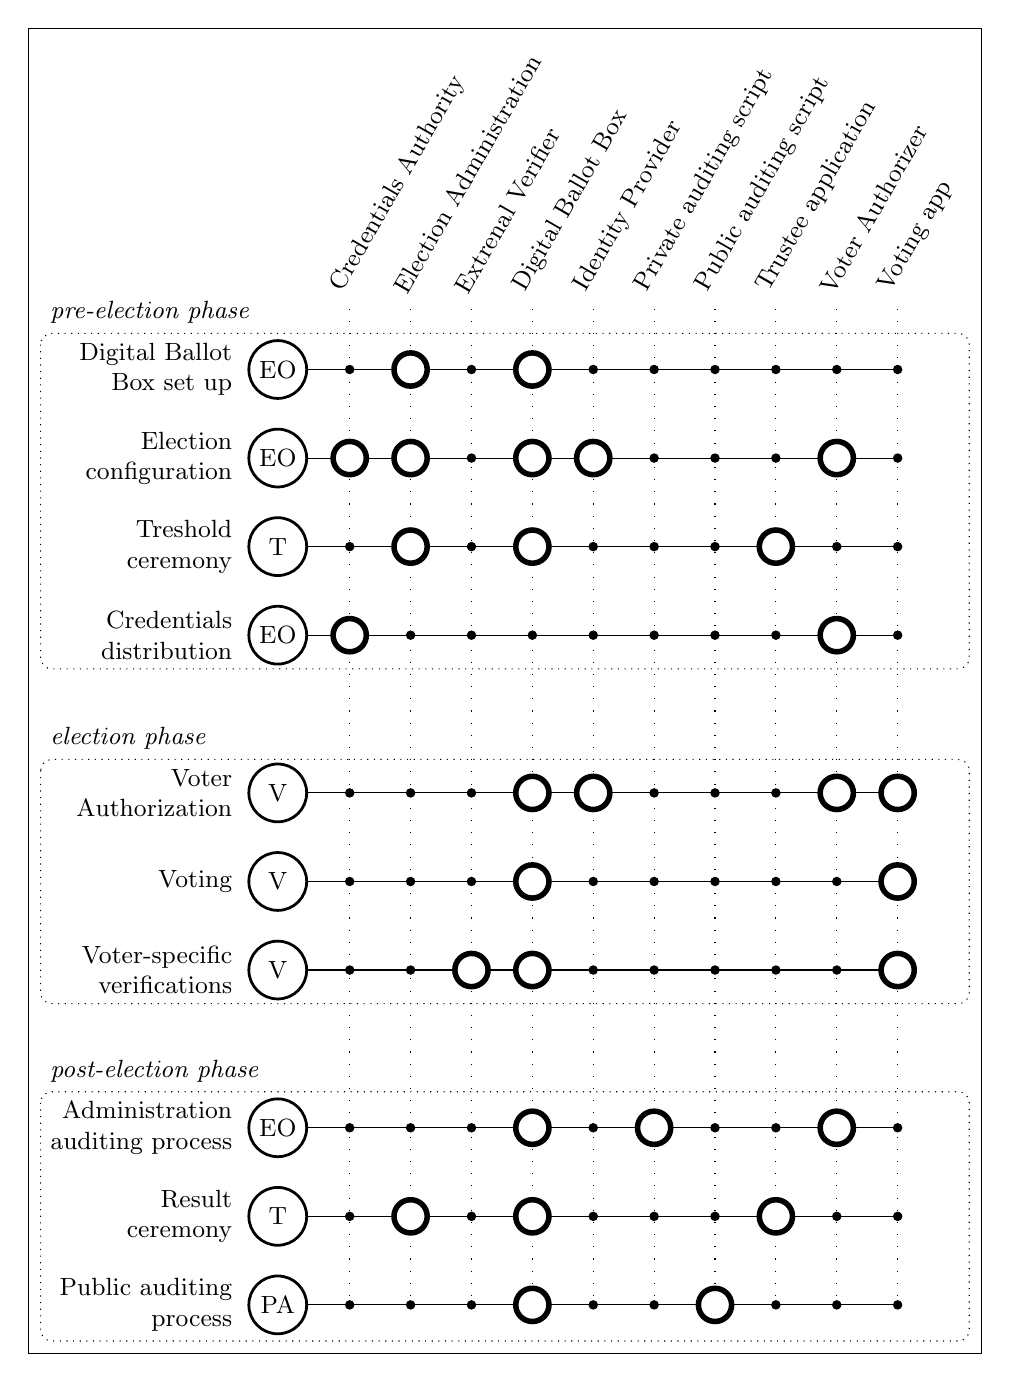
\begin{tikzpicture}[framed, node distance=22pt,
        big_circle/.style={circle, draw, minimum size=12, line width=2, fill=white},
        small_circle/.style={circle, draw, inner sep=0pt, minimum size=3, fill=black},
        label_circle/.style={circle, draw, font=\small, inner sep=0pt, text width=20, xshift=-4pt, line width=1, align=center, fill=white},
        component/.style={font=\small, rotate=60, align=left},
        process/.style={font=\small, xshift=20pt, align=right},
        spaced/.style={yshift=-10pt},
        very_spaced/.style={yshift=-35pt}
        ]{
            \node[small_circle](di_ca){};
            \node[big_circle, right=of di_ca.center, anchor=center](di_ea){};
            \node[small_circle, right=of di_ea.center, anchor=center](di_ev){};
            \node[big_circle, right=of di_ev.center, anchor=center](di_dbb){};
            \node[small_circle, right=of di_dbb.center, anchor=center](di_ip){};
            \node[small_circle, right=of di_ip.center, anchor=center](di_privas){};
            \node[small_circle, right=of di_privas.center, anchor=center](di_pubas){};
            \node[small_circle, right=of di_pubas.center, anchor=center](di_ta){};
            \node[small_circle, right=of di_ta.center, anchor=center](di_va){};
            \node[small_circle, right=of di_va.center, anchor=center](di_votea){};

            \node[big_circle, spaced, below=of di_ca.center, anchor=center](ec_ca){};
            \node[big_circle, right=of ec_ca.center, anchor=center](ec_ea){};
            \node[small_circle, right=of ec_ea.center, anchor=center](ec_ev){};
            \node[big_circle, right=of ec_ev.center, anchor=center](ec_dbb){};
            \node[big_circle, right=of ec_dbb.center, anchor=center](ec_ip){};
            \node[small_circle, right=of ec_ip.center, anchor=center](ec_privas){};
            \node[small_circle, right=of ec_privas.center, anchor=center](ec_pubas){};
            \node[small_circle, right=of ec_pubas.center, anchor=center](ec_ta){};
            \node[big_circle, right=of ec_ta.center, anchor=center](ec_va){};
            \node[small_circle, right=of ec_va.center, anchor=center](ec_votea){};
            
            \node[small_circle, spaced, below=of ec_ca.center, anchor=center](tc_ca){};
            \node[big_circle, right=of tc_ca.center, anchor=center](tc_ea){};
            \node[small_circle, right=of tc_ea.center, anchor=center](tc_ev){};
            \node[big_circle, right=of tc_ev.center, anchor=center](tc_dbb){};
            \node[small_circle, right=of tc_dbb.center, anchor=center](tc_ip){};
            \node[small_circle, right=of tc_ip.center, anchor=center](tc_privas){};
            \node[small_circle, right=of tc_privas.center, anchor=center](tc_pubas){};
            \node[big_circle, right=of tc_pubas.center, anchor=center](tc_ta){};
            \node[small_circle, right=of tc_ta.center, anchor=center](tc_va){};
            \node[small_circle, right=of tc_va.center, anchor=center](tc_votea){};

            \node[big_circle, spaced, below=of tc_ca.center, anchor=center](cd_ca){};
            \node[small_circle, right=of cd_ca.center, anchor=center](cd_ea){};
            \node[small_circle, right=of cd_ea.center, anchor=center](cd_ev){};
            \node[small_circle, right=of cd_ev.center, anchor=center](cd_dbb){};
            \node[small_circle, right=of cd_dbb.center, anchor=center](cd_ip){};
            \node[small_circle, right=of cd_ip.center, anchor=center](cd_privas){};
            \node[small_circle, right=of cd_privas.center, anchor=center](cd_pubas){};
            \node[small_circle, right=of cd_pubas.center, anchor=center](cd_ta){};
            \node[big_circle, right=of cd_ta.center, anchor=center](cd_va){};
            \node[small_circle, right=of cd_va.center, anchor=center](cd_votea){};

            \node[small_circle, very_spaced, below=of cd_ca.center, anchor=center](vap_ca){};
            \node[small_circle, right=of vap_ca.center, anchor=center](vap_ea){};
            \node[small_circle, right=of vap_ea.center, anchor=center](vap_ev){};
            \node[big_circle, right=of vap_ev.center, anchor=center](vap_dbb){};
            \node[big_circle, right=of vap_dbb.center, anchor=center](vap_ip){};
            \node[small_circle, right=of vap_ip.center, anchor=center](vap_privas){};
            \node[small_circle, right=of vap_privas.center, anchor=center](vap_pubas){};
            \node[small_circle, right=of vap_pubas.center, anchor=center](vap_ta){};
            \node[big_circle, right=of vap_ta.center, anchor=center](vap_va){};
            \node[big_circle, right=of vap_va.center, anchor=center](vap_votea){};

            \node[small_circle, spaced, below=of vap_ca.center, anchor=center](v_ca){};
            \node[small_circle, right=of v_ca.center, anchor=center](v_ea){};
            \node[small_circle, right=of v_ea.center, anchor=center](v_ev){};
            \node[big_circle, right=of v_ev.center, anchor=center](v_dbb){};
            \node[small_circle, right=of v_dbb.center, anchor=center](v_ip){};
            \node[small_circle, right=of v_ip.center, anchor=center](v_privas){};
            \node[small_circle, right=of v_privas.center, anchor=center](v_pubas){};
            \node[small_circle, right=of v_pubas.center, anchor=center](v_ta){};
            \node[small_circle, right=of v_ta.center, anchor=center](v_va){};
            \node[big_circle, right=of v_va.center, anchor=center](v_votea){};

            \node[small_circle, spaced, below=of v_ca.center, anchor=center](vsv_ca){};
            \node[small_circle, right=of vsv_ca.center, anchor=center](vsv_ea){};
            \node[big_circle, right=of vsv_ea.center, anchor=center](vsv_ev){};
            \node[big_circle, right=of vsv_ev.center, anchor=center](vsv_dbb){};
            \node[small_circle, right=of vsv_dbb.center, anchor=center](vsv_ip){};
            \node[small_circle, right=of vsv_ip.center, anchor=center](vsv_privas){};
            \node[small_circle, right=of vsv_privas.center, anchor=center](vsv_pubas){};
            \node[small_circle, right=of vsv_pubas.center, anchor=center](vsv_ta){};
            \node[small_circle, right=of vsv_ta.center, anchor=center](vsv_va){};
            \node[big_circle, right=of vsv_va.center, anchor=center](vsv_votea){};

            \node[small_circle, very_spaced, below=of vsv_ca.center, anchor=center](privap_ca){};
            \node[small_circle, right=of privap_ca.center, anchor=center](privap_ea){};
            \node[small_circle, right=of privap_ea.center, anchor=center](privap_ev){};
            \node[big_circle, right=of privap_ev.center, anchor=center](privap_dbb){};
            \node[small_circle, right=of privap_dbb.center, anchor=center](privap_ip){};
            \node[big_circle, right=of privap_ip.center, anchor=center](privap_privas){};
            \node[small_circle, right=of privap_privas.center, anchor=center](privap_pubas){};
            \node[small_circle, right=of privap_pubas.center, anchor=center](privap_ta){};
            \node[big_circle, right=of privap_ta.center, anchor=center](privap_va){};
            \node[small_circle, right=of privap_va.center, anchor=center](privap_votea){};
            
            \node[small_circle, spaced, below=of privap_ca.center, anchor=center](rc_ca){};
            \node[big_circle, right=of rc_ca.center, anchor=center](rc_ea){};
            \node[small_circle, right=of rc_ea.center, anchor=center](rc_ev){};
            \node[big_circle, right=of rc_ev.center, anchor=center](rc_dbb){};
            \node[small_circle, right=of rc_dbb.center, anchor=center](rc_ip){};
            \node[small_circle, right=of rc_ip.center, anchor=center](rc_privas){};
            \node[small_circle, right=of rc_privas.center, anchor=center](rc_pubas){};
            \node[big_circle, right=of rc_pubas.center, anchor=center](rc_ta){};
            \node[small_circle, right=of rc_ta.center, anchor=center](rc_va){};
            \node[small_circle, right=of rc_va.center, anchor=center](rc_votea){};

            \node[small_circle, spaced, below=of rc_ca.center, anchor=center](pubap_ca){};
            \node[small_circle, right=of pubap_ca.center, anchor=center](pubap_ea){};
            \node[small_circle, right=of pubap_ea.center, anchor=center](pubap_ev){};
            \node[big_circle, right=of pubap_ev.center, anchor=center](pubap_dbb){};
            \node[small_circle, right=of pubap_dbb.center, anchor=center](pubap_ip){};
            \node[small_circle, right=of pubap_ip.center, anchor=center](pubap_privas){};
            \node[big_circle, right=of pubap_privas.center, anchor=center](pubap_pubas){};
            \node[small_circle, right=of pubap_pubas.center, anchor=center](pubap_ta){};
            \node[small_circle, right=of pubap_ta.center, anchor=center](pubap_va){};
            \node[small_circle, right=of pubap_va.center, anchor=center](pubap_votea){};

            
            \node[label_circle, left=of di_ca.center, anchor=center](di_actor) {EO};
            \node[label_circle, left=of ec_ca.center, anchor=center](ec_actor) {EO};
            \node[label_circle, left=of tc_ca.center, anchor=center](tc_actor) {T};
            \node[label_circle, left=of cd_ca.center, anchor=center](cd_actor) {EO};
            \node[label_circle, left=of vap_ca.center, anchor=center](vap_actor) {V};
            \node[label_circle, left=of v_ca.center, anchor=center](v_actor) {V};
            \node[label_circle, left=of vsv_ca.center, anchor=center](vsv_actor) {V};
            \node[label_circle, left=of privap_ca.center, anchor=center](privap_actor) {EO};
            \node[label_circle, left=of rc_ca.center, anchor=center](rc_actor) {T};
            \node[label_circle, left=of pubap_ca.center, anchor=center](pubap_actor) {PA};
            
            \node[process, left=of di_actor, anchor=east](di) {Digital Ballot \\ Box set up};
            \node[process, left=of ec_actor, anchor=east](ec) {Election \\ configuration};
            \node[process, left=of tc_actor, anchor=east](tc) {Treshold \\ ceremony};
            \node[process, left=of cd_actor, anchor=east](cd) {Credentials \\ distribution};
            \node[process, left=of vap_actor, anchor=east](vap) {Voter \\ Authorization};
            \node[process, left=of v_actor, anchor=east](v) {Voting};
            \node[process, left=of vsv_actor, anchor=east](vsv) {Voter-specific \\ verifications};
            \node[process, left=of privap_actor, anchor=east](privap) {Administration \\ auditing process};
            \node[process, left=of rc_actor, anchor=east](rc) {Result \\ ceremony};
            \node[process, left=of pubap_actor, anchor=east](pubap) {Public auditing \\ process};

            \node[component, above=of di_ca.center, anchor=south west] (ca) {Credentials Authority};
            \node[component, above=of di_ea.center, anchor=south west] (ea) {Election Administration};
            \node[component, above=of di_ev.center, anchor=south west] (ev) {Extrenal Verifier};
            \node[component, above=of di_dbb.center, anchor=south west] (dbb) {Digital Ballot Box};
            \node[component, above=of di_ip.center, anchor=south west] (ip) {Identity Provider};
            \node[component, above=of di_privas.center, anchor=south west] (privas) {Private auditing script};
            \node[component, above=of di_pubas.center, anchor=south west] (pubas) {Public auditing script};
            \node[component, above=of di_ta.center, anchor=south west] (ta) {Trustee application};
            \node[component, above=of di_va.center, anchor=south west] (va) {Voter Authorizer};
            \node[component, above=of di_votea.center, anchor=south west] (votea) {Voting app};

            \begin{scope}[on background layer]
                \draw (di_actor.center)--(di_votea.center);
                \draw (ec_actor.center)--(ec_votea.center);
                \draw (tc_actor.center)--(tc_votea.center);
                \draw (cd_actor.center)--(cd_votea.center);
                \draw (vap_actor.center)--(vap_votea.center);
                \draw (v_actor.center)--(v_votea.center);
                \draw (vsv_actor.center)--(vsv_votea.center);
                \draw (privap_actor.center)--(privap_votea.center);
                \draw (rc_actor.center)--(rc_votea.center);
                \draw (pubap_actor.center)--(pubap_votea.center);

                \draw[loosely dotted] (ca.south west -| ec_ca.center)--(pubap_ca.center);
                \draw[loosely dotted] (ea.south west -| ec_ea.center)--(pubap_ea.center);
                \draw[loosely dotted] (ev.south west -| ec_ev.center)--(pubap_ev.center);
                \draw[loosely dotted] (dbb.south west -| ec_dbb.center)--(pubap_dbb.center);
                \draw[loosely dotted] (ip.south west -| ec_ip.center)--(pubap_ip.center);
                \draw[loosely dotted] (privas.south west -| ec_privas.center)--(pubap_privas.center);
                \draw[loosely dotted] (pubas.south west -| ec_pubas.center)--(pubap_pubas.center);
                \draw[loosely dotted] (ta.south west -| ec_ta.center)--(pubap_ta.center);
                \draw[loosely dotted] (va.south west -| ec_va.center)--(pubap_va.center);
                \draw[loosely dotted] (votea.south west -| ec_votea.center)--(pubap_votea.center);

                \draw[rounded corners, dotted] (di.north -| privap.west) rectangle (cd.south -| votea.south east);
                \node[font=\small, anchor=south west] at (di.north -| privap.west) {\textit{pre-election phase}};

                \draw[rounded corners, dotted] (vap.north -| privap.west) rectangle (vsv.south -| votea.south east);
                \node[font=\small, anchor=south west] at (vap.north -| privap.west) {\textit{election phase}};

                \draw[rounded corners, dotted] (privap.north -| privap.west) rectangle (pubap.south -| votea.south east);
                \node[font=\small, anchor=south west] at (privap.north -| privap.west) {\textit{post-election phase}};
            \end{scope}    
        }
    \end{tikzpicture}
    \caption{Processes map}
    \label{fig: processes map}
\end{figure}

\subsection{Pre-election phase} \label{sec: pre-election phase}
During the \textit{pre-election phase} human election officers use the Election Administrator service to configure and setup a new election. That consists of the following steps:
\begin{itemize}
    \item initiate a new bulletin board as described in \cref{sec: digital ballot box initialization},
    \item define election level configuration, including election title, contest titles, candidates and other services required in the election, as decribed in \cref{sec: election configuration},
    \item define eligible voters and configure voter authorization mode as decribed in \cref{sec: voter authorization configuration},
    \item facilitate the threshold ceremony as described in \cref{sec: threshold ceremony},
    \item configure the election phase by setting up voting rounds as in \cref{sec: voting rounds}.
\end{itemize}


\subsubsection{Digital Ballot Box initialization} \label{sec: digital ballot box initialization}
An election officer decides the elliptic curve domain parameters $(p, a, b, G, q, h)$ and, according to that, the election administrator service generates a new key pair $(x_\mathcal{E}, Y_\mathcal{E}) \gets \mathsf{KeyGen}()$ (\cref{alg: key gen}), where $x_\mathcal{E}$ is its signing key and will be kept secret throughout the election, and $Y_\mathcal{E}$ is its public signature verification key. Then, the election administrator requests the digital ballot box to initialize a new bulletin board with the initial election meta-data configuration (including the elliptic curve domain parameters and the public key $Y_\mathcal{E}$). A predefined set of elliptic curve domain parameters is listed in \cref{app: supported elliptic curves}.

On this request, the digital ballot box generates a new key pair $(x_\mathcal{D}, Y_\mathcal{D}) \gets \mathsf{KeyGen}()$ (\cref{alg: key gen}), where $x_\mathcal{D}$ is its signing key and will be kept secret throughout the election period, and $Y_\mathcal{D}$ is its public signature verification key. Then, it spawns a new bulletin board by generating a genesis item as the first item of the board $(b_1, \rho_1) \gets \mathtt{WriteOnBoard}(\mathcal{D}, m_1, c_1, p_1)$ (protocol \ref{pro: write on board}), where $m_1 = $ "genesis", $p_1 = \varnothing$ and the content $c_1$ is constructed according to the rules specified in \cref{app: bulletin board item types}. Next, the digital ballot box returns to the election administrator with the freshly created genesis item $b_1$. From this point on, the election administrator service and the digital ballot box represent indentities $\mathcal{E}$ and $\mathcal{D}$ respectivly on the bulletin board.


\subsubsection{Election configuration} \label{sec: election configuration}
Once a bulletin board exists, the election administrator $\mathcal{E}$ can write all the configuration items on the bulletin board by following $\mathtt{WriteOnBoard}(\mathcal{E}, m_i, c_i, p_i)$ (protocol \ref{pro: write on board}). All items are computed and published one by one, based on the rules defined in \cref{app: bulletin board item types}. All items are signed with the election administrator signing key $x_\mathcal{E}$ and they reference as a parent the address of the previous configuration item, i.e. $p_i = h_{i-1}$. The items that make up the initial configuration are:
\begin{itemize}
    \item the election configuration item,
    \item contest configuration items for each contest and
    \item actor configuration items for each other service that needs to interact with the digiutal ballot box, e.g. the voter authorizer or the ballot adjudicator.
\end{itemize}

For each contest, the election officer has to configure a contest identifier, marking rules, result rules and a list of candidates represented by $\boldsymbol{m} = \{ m_1, ..., m_{n_\mathrm{c}} \}$, where $n_\mathrm{c}$ is the number of candidates.

For each actor, the Election Administrator service interacts with the other service, e.g. the voter authorizer, to generate its own key pair $(x_\mathcal{A}, Y_\mathcal{A}) \gets \mathsf{KeyGen}()$ (\cref{alg: key gen}). Value $x_\mathcal{A}$ is the voter authorizer signing key and will be kept secret throughout the election period while $Y_\mathcal{A}$ is its public signature verification key and it is shared with the election administrator. Next, the election administrator assignes the role of \textit{voter authorizer} to the public key $Y_\mathcal{A}$. Once the actor configuration item containing the public key $Y_\mathcal{A}$ is published on the bulletin board, the voter authorizer becomes indentity $\mathcal{A}$ and can interact with the digital ballot box.


\subsubsection{Voter authorization configuration} \label{sec: voter authorization configuration}
An election officer interacts with the Voter Authorizer service to configure the voter authentication mode, which can be either \textbf{credential-based} or \textbf{identity-based}. In order to define the list of eligible voters, the election officer has to perform some extra configuration depending on the voter authentication mode selected previously.

When \textbf{credential-based} voter authentication mode is enabled, the election officer sets up a set of credentials authorities $\boldsymbol{\mathcal{C}} = \{ \mathcal{C}_1, ..., \mathcal{C}_{n_\mathrm{c}} \}$ used for distributing voter credentials, each authority $\mathcal{C}_i \in \boldsymbol{\mathcal{C}}$ being specified to use a particular communication channel for distributing voter credentials, e.g. e-mail, post or SMS. Then the election officer provides the list of eligible voters $\boldsymbol{\mathcal{V}} = \{ \mathcal{V}_1, ..., \mathcal{V}_{n_\mathrm{v}} \}$, where each voter is defined by a unique identifier and a list of contact information for each communication channel used by the credentials authorities.

Next, credentials authorities and the voter authorizer perform the voter credential distribution process (describe in \cref{sec: voter credential distribution process}) and setup the public authentication key of each voter.

Finally, the voter authorizer writes the voter authorization configuration item on the bulletin board by performing $\mathtt{WriteOnBoard}(\mathcal{A}, m_i, c_i, p_i)$ (protocol \ref{pro: write on board}) based on the rules defined in \cref{app: bulletin board item types}. The item is signed by the voter authorizer signing key $x_\mathcal{A}$ and it contains the voter authentication mode.

When \textbf{identity-based} voter authentication mode is enabled, the election officer selects a list of third party identity providers $\boldsymbol{\mathcal{I}} = \{ \mathcal{I}_1, ..., \mathcal{I}_{n_\mathrm{i}} \}$ used for authenticating voters during the election phase. Then the election officer provides the list of eligible voters $\boldsymbol{\mathcal{V}} = \{ \mathcal{V}_1, ..., \mathcal{V}_{n_\mathrm{v}} \}$, where each voter is defined by a unique identifier and a list of identities supported by each of the identity providers.

Finally, the voter authorizer writes the voter authorization configuration item on the bulletin board by following $\mathtt{WriteOnBoard}(\mathcal{A}, m_i, c_i, p_i)$ (protocol \ref{pro: write on board}) based on the rules defined in \cref{app: bulletin board item types}. The item is signed by the voter authorizer signing key $x_\mathcal{A}$ and it contains the voter authentication mode and the list of identity providers $\mathcal{I}_j$, each defined by their public key $Y_{\mathcal{I}_j}$ and a URL, with $j \in \{ 1, ..., n_\mathrm{i} \}$.


\subsubsection{Voter credential distribution process} \label{sec: voter credential distribution process}
This process is only applicable if the vote authentication mode is \textbf{credential-based}, as described in \cref{sec: credential-based mode}.

Each credentials authority $\mathcal{C}_j \in \boldsymbol{\mathcal{C}}$, receives a list of voters consisting of contact details for each voter $\boldsymbol{a} = \{ a_1, ..., a_{n_\mathrm{v}} \}$ in form of e-mail addresses or postal addresses or phone numbers, depending on the credentials authority's communication channel. The credentials authority generates random credentials $c_{i, j} \in_\mathrm{R} \mathbb{B}^\ell$ for each voter, with $i \in \{ 1, ..., n_\mathrm{v} \}$. The credentials authority distributes the credential $c_{i, j}$ to that specific voter $\mathcal{V}_i$ (using voter's contact detail $a_i$) and appends the corresponding public authentication key $Y_{\mathrm{auth}; i, j}$ in the list of voters next to the specific voter $\mathcal{V}_i$, where $(x_{\mathrm{auth}; i, j}, Y_{\mathrm{auth}; i, j}) \gets \mathsf{Pass2Key}(c_{i, j})$ (\cref{alg: pass to key}).

Credential generation can be done in form of a random string of characters or numbers or a combination of them. In any case, it has to be bound by the level of entropy $\ell$. It is recommended that credentials are based on at least 80 bits of entropy, i.e. $\ell \geq 80$. That corresponds to a 14 characters alphanumeric code that has to be sent to the voter and inputted in the voting application.

All credentials authorities $\mathcal{C}_j \in \boldsymbol{\mathcal{C}}$ return to the voter authorizer the lists with voters contact details and public authentication keys $(a_i, Y_{\mathrm{auth}; i,j})$. The voter authorizer combines all keys received from all credentials authorities for each voter to form the voter's public authentication key $Y_{\mathrm{auth}; i} = \sum_{j=1}^{n_\mathrm{c}} Y_{\mathrm{auth}; i, j}$.

For authenticating to the voter authorizer, the voter $\mathcal{V}_i \in \boldsymbol{\mathcal{V}}$ has to input in the voting application all credentials $\{ c_{i, 1}, ..., c_{i, n_\mathrm{c}} \}$ received via different channels from all credentials authorities. The voting application will derive keys from each credential $(x_{\mathrm{auth}; i, j}, Y_{\mathrm{auth}; i, j}) \gets \mathsf{Pass2Key}(c_{i, j})$ (\cref{alg: pass to key}) and aggregate all of them to form the voter's private authentication key $x_{\mathrm{auth}; i} = \sum_{j=1}^{n_\mathrm{c}} x_{\mathrm{auth}; i, j} \pmod q$. The private authentication key is used to compute a proof of credentials $PK_\mathrm{auth}$, as described in \cref{sec: voter authorization procedure}, which is used to authenticate the voter.


\subsubsection{Threshold ceremony} \label{sec: threshold ceremony}
An election officer interacts with the election administrator service to define the lists of trustees $\boldsymbol{\mathcal{T}} = \{ \mathcal{T}_1, ..., \mathcal{T}_{n_\mathrm{t}} \}$. Then, the election administrator coordinates the threshold ceremony during which all trustees $\mathcal{T}_i \in \boldsymbol{\mathcal{T}}$ participate in the protocol from \cref{fig: threshold ceremony} described in \cref{app: threshold cryptosystem} in order to generate the election encryption key $Y_\mathrm{enc}$ and each trustee's share of the decryption key $sx_i$. The election officer sets the threshold value $t$, such that any $t$ out of the $n_\mathrm{t}$ trustees can perform decryption.

At the end of the ceremony, the election administrator writes the threshold configuration item on the bulletin board by following $\mathtt{WriteOnBoard}(\mathcal{E}, m_i, c_i, p_i)$ (protocol \ref{pro: write on board}) based on the rules defined in \cref{app: bulletin board item types}. The item contains:
\begin{itemize}
    \item election encryption key $Y_\mathrm{enc}$,
    \item threshold setup $t$-out-of-$n_\mathrm{t}$,
    \item public keys of each trustee $Y_{\mathcal{T}_i}$, with $i \in \{1, ..., n_\mathrm{t}\}$,
    \item public polynomial coefficients of each trustee $P_{\mathcal{T}_i,j}$, with $j \in \{1, ..., t-1 \}$.
\end{itemize}


\subsubsection{Voting rounds} \label{sec: voting rounds}
An election officer interacts with the election administrator service to define when the election phase is taking place, by setting a start date and an end date. Then, the election administrator $\mathcal{E}$ writes a voting round item on the bulletin board by following $\mathtt{WriteOnBoard}(\mathcal{E}, m_i, c_i, p_i)$ (protocol \ref{pro: write on board}) based on the rules defined in \cref{app: bulletin board item types}, specifying the start and end date and enabling all contest identifiers.

For a regular election, a single voting round is sufficient, but multiple voting rounds can be configured to start at different times and different contests could be enabled in each voting round.

\subsection{Election phase} \label{sec: election phase}
The election phase lasts from the start date until the end date of a voting round. During this time, any voter $\mathcal{V}_i \in \boldsymbol{\mathcal{V}}$ can cast a valid digital ballot by performing the following steps:
\begin{itemize}
    \item get a list with all configuration items of the bulletin board $\alpha_\mathrm{cnf}$ from the digital ballot box,
    \item authenticate and get authorized to cast a digital ballot on the bulletin board as described in \cref{sec: voter authorization procedure},
    \item select vote choices and prepare them for encryption as described in \cref{sec: mapping vote options on the elliptic curve},
    \item encrypt the ballot following the process from \cref{sec: vote cryptogram generation process},
    \item optionally, perform an audit/verification on the encrypted ballot as described in \cref{sec: challenging a vote cryptogram} and
    \item finally, cast the encrypted ballot and obtain a vote confirmation receipt as in \cref{sec: vote confirmation receipt}.
\end{itemize}


\subsubsection{Voter authorization procedure} \label{sec: voter authorization procedure}
A voter $\mathcal{V}_i$ is considered authorized to cast a digital ballot when it is in possession of a secret signing key $x_i$ that corresponds to an eligible signature verification key $Y_i$ from the bulletin board. This is achieved differently depending on the voter authentication mode.


\paragraph{When credential-based voter authentication mode}\mbox{}\\
Each voter $\mathcal{V}_i$ has to follow the protocol from \cref{fig: credential-based voter authentication protocol} in order to get authorized to cast a digital ballot on the bulletin board. Specifically, the voter must prove possession of credentials that are associated with the voter's authentication public key $Y_{\mathrm{auth}; i}$.

Voter inputs to the voting application the credentials received from each credentials authority $\{ c_1, ..., c_{n_\mathrm{c}} \}$. All credentials get converted into the voter's authentication key pair $(x_{\mathrm{auth}; i}, Y_{\mathrm{auth}; i})$, where the private key $x_{\mathrm{auth}; i}$ is computed by adding together all keys derived from each credential $c_j$ (by using \cref{alg: pass to key} $\mathsf{Pass2Key}(c_j)$), with $j \in \{ 1, ..., n_\mathrm{c} \}$. The public key is trivially computed by $Y_{\mathrm{auth}; i} \gets [x_{\mathrm{auth}; i}]G$. Based on the private key, the voting application computes $PK_\mathrm{auth} \gets \mathsf{DLProve} (x_{\mathrm{auth}; i}, \{ G \})$ as the proof of credentials.

Then, the voting application generates a new key pair $(x_i, Y_i)$ to be used as the signing/signature verification keys in the upcoming voter session. The voting application sends the proof $PK_\mathrm{auth}$ and the public key $Y_i$ to the voter authorizer proving possession of credentials of voter $\mathcal{V}_i$. The voter authorizer checks that the proof is valid and whether it was generated by an eligible voter from $\boldsymbol{\mathcal{V}}$.

If the authentication succeeds, the voter authorizer service will authorize the use of public key $Y_i$ for the voter $\mathcal{V}_i$ by interacting with the digital ballot box $\mathcal{D}$ in $\mathtt{WriteOnBoard}(\mathcal{A}, m_\mathrm{vs}, c_\mathrm{vs}, p_\mathrm{vs})$ (protocol \ref{pro: write on board}) to write a voter session item $b_\mathrm{vs}$ as the next item on the bulletin board, according to the rules specified in \cref{app: bulletin board item types}, where $m_\mathrm{vs} =$ "voter session", the parent $p_\mathrm{vs}$ is the address of the latest configuration item and the content $c_\mathrm{vs}$ consists of the voter identifier, the public key $Y_i$, and a digest of the proof $PK_\mathrm{auth}$.

The voter authorizer returns to the voter with the voter session item $b_\mathrm{vs}$ as received from the digital ballot box. The voting application validates the item according to protocol \ref{pro: write on board}. Additionally, it checks that the item is consistent according to the configuration ancestry $\alpha_\mathrm{cnf}$ (i.e. $\mathsf{AncestryVer}(\{ b_\mathrm{vs} \}, h_\mathrm{cnf})$, where $h_\mathrm{cnf}$ is the address of the last item in $\alpha_\mathrm{cnf}$). From this point on, the voter can interact directly with the digital ballot box as the identity $\mathcal{V}_i$.

The voter authorizer service stores a link between the voter identity $\mathcal{V}_i$ and the proof of credentials $PK_\mathrm{auth}$ for the purpose of the administration auditing process in the post-election phase as described in \cref{sec: administration auditing process}.

\begin{figure}[ht]
    \centering
    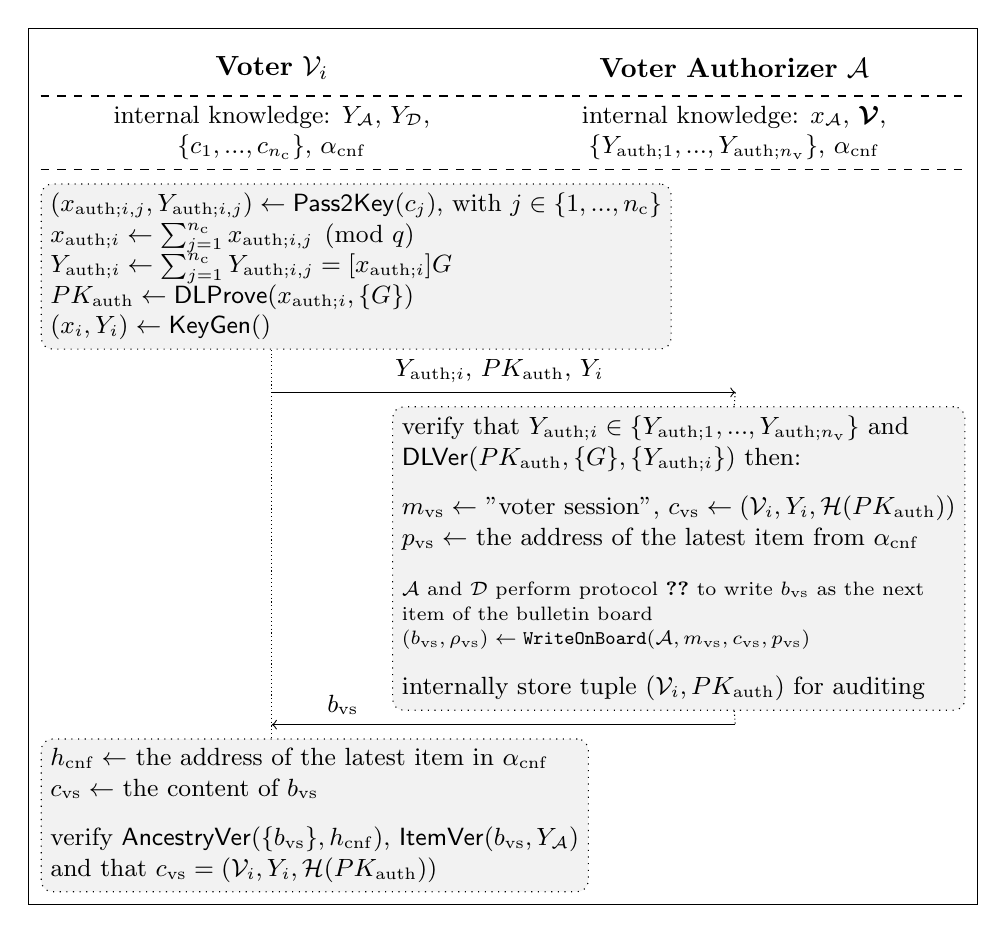
\begin{tikzpicture}[framed, node distance=0,
            spaced/.style={yshift=-5},
            % every node/.style={draw},
            ]{
        
        % Actors
        \node[title, above, anchor=north east] (v) {
            \textbf{Voter $\mathcal{V}_i$}};
        \node[title, right=of v] (va) {
            \textbf{Voter Authorizer $\mathcal{A}$}};
        
        % internal knowledge
        \node[ik] at (v.south) (v_ik) {
            internal knowledge: $Y_\mathcal{A}$, $Y_\mathcal{D}$, \\
            $\{ c_1, ..., c_{n_\mathrm{c}} \}$, $\alpha_\mathrm{cnf}$
            };
        \node[ik] at (va.south) (va_ik) {
            internal knowledge: $x_\mathcal{A}$, $\boldsymbol{\mathcal{V}}$, \\
            $\{ Y_{\mathrm{auth}; 1}, ..., Y_{\mathrm{auth}; n_\mathrm{v}} \}$, $\alpha_\mathrm{cnf}$
            };
        
        % All content
        \node[block, keep_left, spaced] at (v_ik.south -| v.west) (v_1) {
            $(x_{\mathrm{auth}; i, j}, Y_{\mathrm{auth}; i, j}) \gets \mathsf{Pass2Key}(c_j)$, with $j \in \{ 1, ..., n_\mathrm{c} \}$ \\
            $x_{\mathrm{auth}; i} \gets \sum_{j=1}^{n_\mathrm{c}} x_{\mathrm{auth}; i, j} \pmod{q}$ \\
            $Y_{\mathrm{auth}; i} \gets \sum_{j=1}^{n_\mathrm{c}} Y_{\mathrm{auth}; i, j} = [x_{\mathrm{auth}; i}]G$ \\
            $PK_\mathrm{auth} \gets \mathsf{DLProve} (x_{\mathrm{auth}; i}, \{ G \})$ \\
            $(x_i, Y_i) \gets \mathsf{KeyGen} ()$
            };
        \node[arrow, towards_right, between={v.center}{va.center}] at (v_1.south -| v.center) (a_1) {
            $Y_{\mathrm{auth}; i}$, $PK_\mathrm{auth}$, $Y_i$
            };
        \node[block, keep_right, spaced] at (a_1.south -| va.east) (va_1) {
            verify that $Y_{\mathrm{auth}; i} \in \{ Y_{\mathrm{auth}; 1}, ..., Y_{\mathrm{auth}; n_\mathrm{v}} \}$ and \\
            $\mathsf{DLVer} (PK_\mathrm{auth}, \{ G \}, \{ Y_{\mathrm{auth}; i} \})$ then: \\ [7pt]
            $m_\mathrm{vs} \gets$ "voter session", $c_\mathrm{vs} \gets (\mathcal{V}_i, Y_i, \mathcal{H}(PK_\mathrm{auth}))$ \\
            $p_\mathrm{vs} \gets$ the address of the latest item from $\alpha_\mathrm{cnf}$ \\ [7pt]
            \scriptsize $\mathcal{A}$ and $\mathcal{D}$ perform protocol \ref{pro: write on board} to write $b_\mathrm{vs}$ as the next \\ [-2pt]
            \scriptsize item of the bulletin board \\ [-2pt]
            \scriptsize $(b_\mathrm{vs}, \rho_\mathrm{vs}) \gets \mathtt{WriteOnBoard}(\mathcal{A}, m_\mathrm{vs}, c_\mathrm{vs}, p_\mathrm{vs})$ \\ [7pt]
            internally store tuple $(\mathcal{V}_i, PK_\mathrm{auth})$ for auditing
            };
        \node[arrow, towards_left, immediate, between={v.center}{va.center}] at (va_1.south -| v.center) (a_2) {
            $b_\mathrm{vs}$ \hspace{110pt}
            };
        \node[block, keep_left, spaced] at (a_2.south -| v.west) (v_2) {
            $h_\mathrm{cnf} \gets $ the address of the latest item in $\alpha_\mathrm{cnf}$ \\
            $c_\mathrm{vs} \gets $ the content of $b_\mathrm{vs}$ \\ [7pt]
            verify $\mathsf{AncestryVer}(\{ b_\mathrm{vs} \}, h_\mathrm{cnf})$, $\mathsf{ItemVer}(b_\mathrm{vs}, Y_\mathcal{A})$ \\
            and that $c_\mathrm{vs} = (\mathcal{V}_i, Y_i, \mathcal{H}(PK_\mathrm{auth}))$
            };
        
        % Arrows and lines
        \draw[dashed] (v.south west)--(va.south east);    
        \draw[dashed] (v_ik.south -| v.west)--(v_ik.south -| va.east);
        
        \draw[densely dotted] (v_1.south -| v.center)--(v_2.north -| v.center);

        \draw[densely dotted] (a_1.south east)--(va_1.north -| va.center);
        \draw[densely dotted] (va_1.south -| va.center)--(a_2.south east);
        }
    \end{tikzpicture}
    \caption{\textbf{Credential-based} voter authentication protocol}
    \label{fig: credential-based voter authentication protocol}
\end{figure}


\paragraph{When identity-based voter athentication mode}\mbox{}\\
Each voter $\mathcal{V}_i$ has to follow the protocol from \cref{fig: identity-based voter authentication protocol} in order to get authorized to cast a digital ballot on the bulletin board. Specifically, the voter must authenticate and get identity tokens $\sigma_{\mathrm{id}, j}$ from all of the idenitity providers $\mathcal{I}_j \in \boldsymbol{\mathcal{I}}$ that have been configured by the voter authorizer in the pre-election phase.

Then, the voting application generates a key pair $(x_i, Y_i) \gets \mathsf{KeyGen}()$ (\cref{alg: key gen}) and forwards all identity tokens $\{ \sigma_{\mathrm{id}, 1}, ..., \sigma_{\mathrm{id}, n_\mathrm{i}} \}$ and the public key $Y_i$ to the voter authorizer service $\mathcal{A}$ proving the identity of the voter $\mathcal{V}_i$.

If the voter authorizer service can validate all identity tokens and the voter is eligible, i.e. $\mathcal{V}_i \in \boldsymbol{\mathcal{V}}$, then it will authorize the use of the public key $Y_i$ for the voter $\mathcal{V}_i$. This is done by the voter authorizer $\mathcal{A}$ interacting with the digital ballot box $\mathcal{D}$ in the protocol \ref{pro: write on board} $\mathtt{WriteOnBoard}(\mathcal{A}, m_\mathrm{vs}, c_\mathrm{vs}, p_\mathrm{vs})$ to write a voter session item $b_\mathrm{vs}$ on the bulletin board as the next item, according to the rules specified in \cref{app: bulletin board item types}, where $m_\mathrm{vs} =$ "voter session", the parent $p_\mathrm{vs}$ is the address of the latest configuration item and the content $c_\mathrm{vs}$ consists of the voter identifier, the public key $Y_i$, and the authentication fingerprint computed by hashing all identity tokens received from the voter. 

The voter authorizer returns to the voter the voter session item $b_\mathrm{vs}$ as received from the digital ballot box. The voting application checks the item according to the validations of protocol \ref{pro: write on board}. Additionally, it checks that the item is consistent according to the configuration ancestry $\alpha_\mathrm{cnf}$ (i.e. $\mathsf{AncestryVer}(\{ b_\mathrm{vs} \}, h_\mathrm{cnf})$, where $h_\mathrm{cnf}$ is the address of the last item in $\alpha_\mathrm{cnf}$). From this point on, the voter can interact directly with the digital ballot box as the identity $\mathcal{V}_i$.

The voter authorizer service stores a link between the voter identity $\mathcal{V}_i$ and all related identity tokens for the purpose of the private auditing process in the post-election phase as described in \cref{sec: administration auditing process}. This link is stored privately by the voter authorizer service due to the fact that the identity tokens likely contain personal information that must not be disclosed on the public bulletin board.

\clearpage
\begin{landscape}
\begin{figure}[ht]
    \centering
    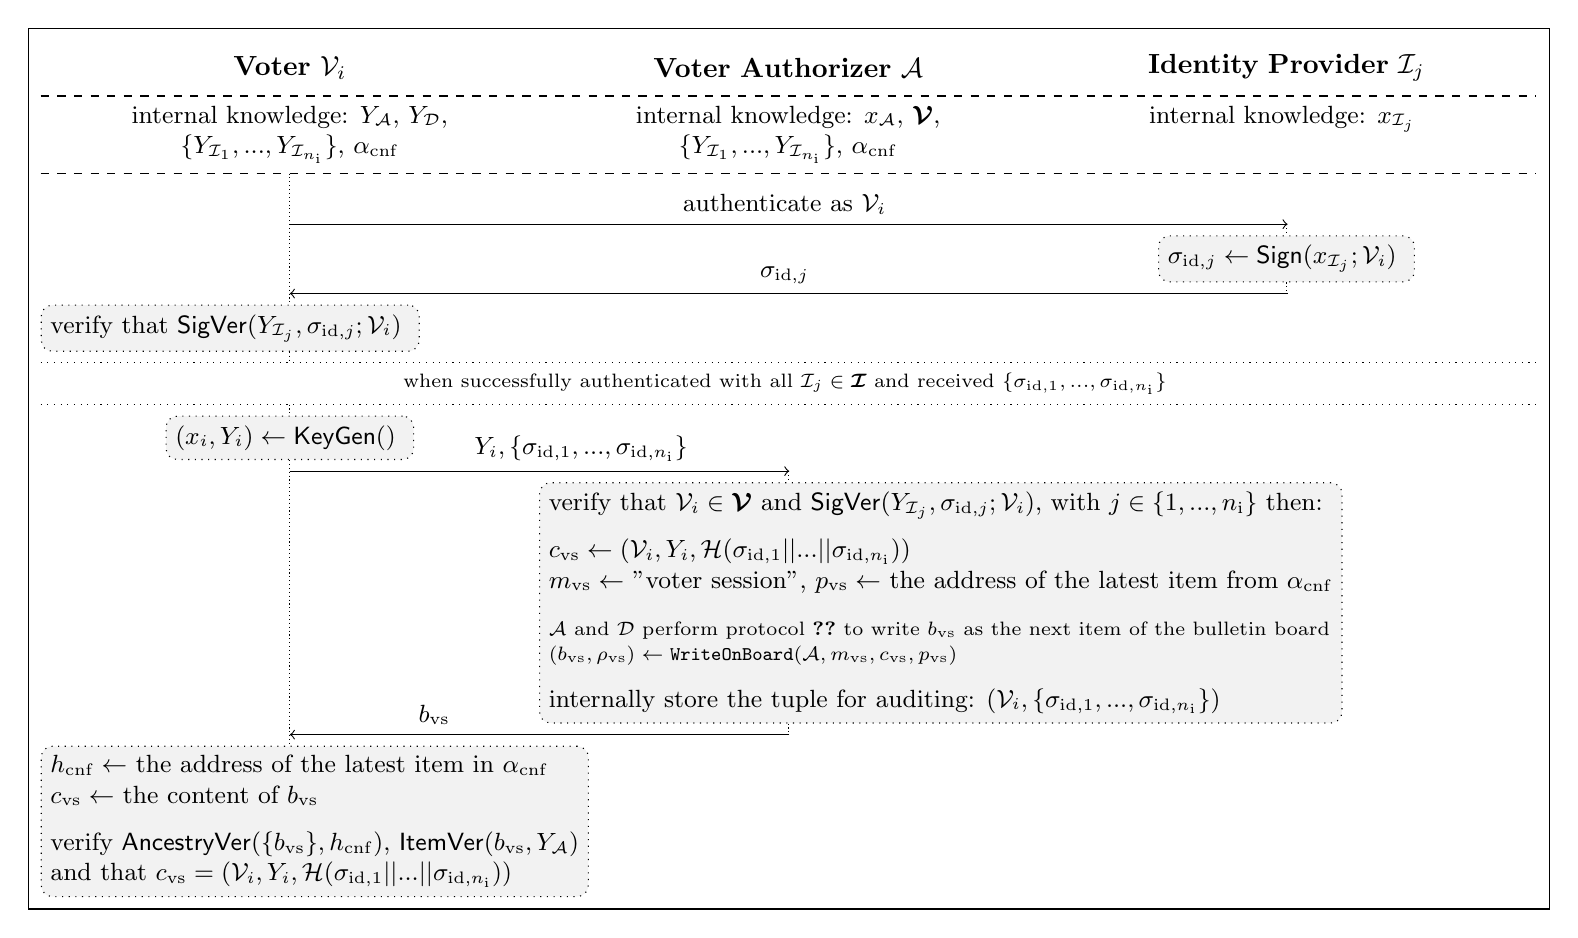
\begin{tikzpicture}[framed, node distance=0,
            spaced/.style={yshift=-4},
            % every node/.style={draw},
            ]{
        
        % Actors
        \node[title_3, above, anchor=north east] (v) {
            \textbf{Voter $\mathcal{V}_i$}};
        \node[title_3, right=of v] (va) {
            \textbf{Voter Authorizer $\mathcal{A}$}};
        \node[title_3, right=of va] (ip) {
            \textbf{Identity Provider $\mathcal{I}_j$}};
        
        % internal knowledge
        \node[ik] at (v.south) (v_ik) {
            internal knowledge: $Y_\mathcal{A}$, $Y_\mathcal{D}$, \\
            $\{ Y_{\mathcal{I}_1}, ..., Y_{\mathcal{I}_{n_\mathrm{i}}} \}$, $\alpha_\mathrm{cnf}$
            };
        \node[ik] at (va.south) (va_ik) {
            internal knowledge: $x_\mathcal{A}$, $\boldsymbol{\mathcal{V}}$, \\
            $\{ Y_{\mathcal{I}_1}, ..., Y_{\mathcal{I}_{n_\mathrm{i}}} \}$, $\alpha_\mathrm{cnf}$
            };
        \node[ik] at (ip.south) (ip_ik) {
            internal knowledge: $x_{\mathcal{I}_j}$
            };
        
        % All content
        \node[arrow, towards_right, spaced, between={v.center}{ip.center}] at (v_ik.south -| v.center) (a_1) {
            authenticate as $\mathcal{V}_i$
            };
        \node[block, keep_middle, spaced] at (a_1.south -| ip.center) (ip_1) {
            $\sigma_{\mathrm{id}, j} \gets \mathsf{Sign}(x_{\mathcal{I}_j}; \mathcal{V}_i)$
            };
        \node[arrow, towards_left, immediate, between={v.center}{ip.center}] at (ip_1.south -| v.center) (a_2) {
            $\sigma_{\mathrm{id}, j}$
            };
        \node[block, keep_left, spaced] at (a_2.south -| v.west) (v_1) {
            verify that $\mathsf{SigVer}(Y_{\mathcal{I}_j}, \sigma_{\mathrm{id}, j}; \mathcal{V}_i)$
            };
        \node[banner, keep_left, spaced, between={v.west}{ip.east}] at (v_1.south -| v.west) (b_1) {
            when successfully authenticated with all $\mathcal{I}_j \in \boldsymbol{\mathcal{I}}$ and received $\{ \sigma_{\mathrm{id}, 1}, ..., \sigma_{\mathrm{id}, n_\mathrm{i}} \}$
            };
        \node[block, keep_middle, spaced] at (b_1.south -| v.center) (v_2) {
            $(x_i, Y_i) \gets \mathsf{KeyGen}()$
            };
        \node[arrow, towards_right, immediate, between={v.center}{va.center}] at (v_2.south -| v.center) (a_3) {
            \hspace{30pt} $Y_i, \{ \sigma_{\mathrm{id}, 1}, ..., \sigma_{\mathrm{id}, n_\mathrm{i}} \}$
            };
        \node[block, keep_left, spaced] at (a_3.south -| va.west) (va_1) {
            verify that $\mathcal{V}_i \in \boldsymbol{\mathcal{V}}$ and $\mathsf{SigVer}(Y_{\mathcal{I}_j}, \sigma_{\mathrm{id}, j}; \mathcal{V}_i)$, with $j \in \{1, ..., n_\mathrm{i}\}$ then: \\ [6pt]
            $c_\mathrm{vs} \gets (\mathcal{V}_i, Y_i, \mathcal{H}(\sigma_{\mathrm{id}, 1} || ... || \sigma_{\mathrm{id}, n_\mathrm{i}}))$ \\
            $m_\mathrm{vs} \gets$ "voter session", $p_\mathrm{vs} \gets$ the address of the latest item from $\alpha_\mathrm{cnf}$ \\ [6pt]
            \scriptsize $\mathcal{A}$ and $\mathcal{D}$ perform protocol \ref{pro: write on board} to write $b_\mathrm{vs}$ as the next item of the bulletin board \\ [-2pt]
            \scriptsize $(b_\mathrm{vs}, \rho_\mathrm{vs}) \gets \mathtt{WriteOnBoard}(\mathcal{A}, m_\mathrm{vs}, c_\mathrm{vs}, p_\mathrm{vs})$ \\ [6pt]
            internally store the tuple for auditing: $(\mathcal{V}_i, \{ \sigma_{\mathrm{id}, 1}, ..., \sigma_{\mathrm{id}, n_\mathrm{i}} \})$
            };
        \node[arrow, towards_left, immediate, between={v.center}{va.center}] at (va_1.south -| v.center) (a_4) {
            $b_\mathrm{vs}$ \hspace{70pt}
            };
        \node[block, keep_left, spaced] at (a_4.south -| v.west) (v_3) {
            $h_\mathrm{cnf} \gets $ the address of the latest item in $\alpha_\mathrm{cnf}$ \\
            $c_\mathrm{vs} \gets $ the content of $b_\mathrm{vs}$ \\ [6pt]
            verify $\mathsf{AncestryVer}(\{ b_\mathrm{vs} \}, h_\mathrm{cnf})$, $\mathsf{ItemVer}(b_\mathrm{vs}, Y_\mathcal{A})$ \\
            and that $c_\mathrm{vs} = (\mathcal{V}_i, Y_i, \mathcal{H}(\sigma_{\mathrm{id}, 1} || ... || \sigma_{\mathrm{id}, n_\mathrm{i}}))$
            };
        
        % Arrows and lines
        \draw[dashed] (v.south west)--(ip.south east);    
        \draw[dashed] (v_ik.south -| v.west)--(v_ik.south -| ip.east);
        
        \draw[dotted] (b_1.north west)--(b_1.north east);
        \draw[dotted] (b_1.south west)--(b_1.south east);
        
        \draw[densely dotted] (v_ik.south -| v.center)--(v_1.north -| v.center);
        \draw[densely dotted] (v_1.south -| v.center)--(b_1.north -| v.center);
        \draw[densely dotted] (b_1.south -| v.center)--(v_2.north -| v.center);
        \draw[densely dotted] (v_2.south -| v.center)--(v_3.north -| v.center);

        \draw[densely dotted] (a_3.south -| va.center)--(va_1.north -| va.center);
        \draw[densely dotted] (va_1.south -| va.center)--(a_4.south -| va.center);

        \draw[densely dotted] (a_1.south -| ip.center)--(ip_1.north -| ip.center);
        \draw[densely dotted] (ip_1.south -| ip.center)--(a_2.south -| ip.center);
        }
    \end{tikzpicture}
    \caption{\textbf{Identity-based} voter authentication protocol}
    \label{fig: identity-based voter authentication protocol}
\end{figure}
\end{landscape}


\clearpage
\subsubsection{Mapping vote options on the Elliptic Curve} \label{sec: mapping vote options on the elliptic curve}
An expressed vote (i.e., a vote in plain text) must be able to be converted deterministically into elliptic curve points to be used in our cryptographic protocols. Additionally, a series of points from the elliptic curve must be able to be turned back into a plain-text vote if the points have been constructed from a plain-text vote. Depending on the election type (referendum, simple election, multiple choice election, STV election), the plain text vote can be constructed in different ways, for example, a simple string, an array of integers, or even a complex data structure. Regardless of the vote encoding rules, the plain-text vote has a byte representation $\vec{b} \in \mathbb{B}^*$.

Next, $\vec{b}$ is converted into elliptic curve points $\vec{V} \gets \mathsf{EncodeVote}(\vec{b})$ (\cref{alg: encode vote}), which can be used in the encryption mechanism described in \cref{sec: vote cryptogram generation process}. Thus, the set of points $\vec{V}$ represents the voter's choices in cryptographic form.

Recovering the byte array $\vec{b}$ from $\vec{V}$ can be done by $\vec{b} \gets \mathsf{DecodeVote}(\vec{V})$ (\cref{alg: decode vote}). Depending on the vote encoding rules, the byte array $\vec{b}$ can further be interpreted as a plain-text vote.

\begin{algorithm}[ht]
    \DontPrintSemicolon
    \caption{$\mathsf{EncodeVote} (\vec{b})$}
    \label{alg: encode vote}
    \KwData{The plain-text vote $\vec{b} = \{ b_1, ..., b_n \} \in \mathbb{B}^n$}
    
    $m \gets \mathsf{ByteLengthOf} (p)$  \;
    $\ell \gets \lceil n / m \rceil$ \;
    \For{$i \gets 0$ \KwTo $\ell - 1$ \KwBy $1$}{
        $V_i \gets \mathsf{Bytes2Point} (\{ b_{i+1}, ..., b_{i+m} \})$ \;
        }
    $\vec{V} \gets \{ V_1, ..., V_\ell \}$ \;
    \Return{$\vec{V}$} \tcp*{$\vec{V} \in \mathbb{P}^*$}
\end{algorithm}

\begin{algorithm}[ht]
    \DontPrintSemicolon
    \caption{$\mathsf{DecodeVote} (\vec{V})$}
    \label{alg: decode vote}
    \KwData{The list of points $\vec{V} = \{ V_1, ..., V_\ell \} \in \mathbb{P}^\ell$}
    
    $\vec{b} \gets \{ \}$  \;
    \For{$i \gets 1$ \KwTo $\ell$ \KwBy $1$}{
        $\vec{b} \gets \vec{b} \cup \mathsf{Point2Bytes} (V_i)$ \;
        }
    \Return{$\vec{b}$} \tcp*{$\vec{b} \in \mathbb{B}^*$}
\end{algorithm}


\subsubsection{Vote cryptogram generation process} \label{sec: vote cryptogram generation process}
During the vote cryptogram generation process, the voting application collaborates with the digital ballot box $\mathcal{D}$ for generating the cryptogram $e$ that represents the encryption of the vote $M$. This process results in the fact that neither the voter $\mathcal{V}_i$ nor the digital ballot box $\mathcal{D}$ will be in possession of whole randomizer value $r$ used in the generation process of cryptogram $e$ (recall from \cref{app: encryption scheme} that $e = \mathsf{Enc}(Y_\mathrm{enc}, M; r)$). That is achieved by both the voter and the digital ballot box building up the randomizer but none of them knowing its entire value. It is important for the voter to not know this value in order to not be able to produce cryptographic evidence of the way he voted (as in \cref{app: proving the content of a cryptogram}), thus achieving \textit{receipt freeness}. The entire process cosists of commiting to the encryption randomizers which is presented in \cref{fig: encryption commitments submission protocol} and submitting the encrypted ballot as presented in \cref{fig: encrypted ballot submission protocol}.

\begin{figure}[ht]
    \centering
    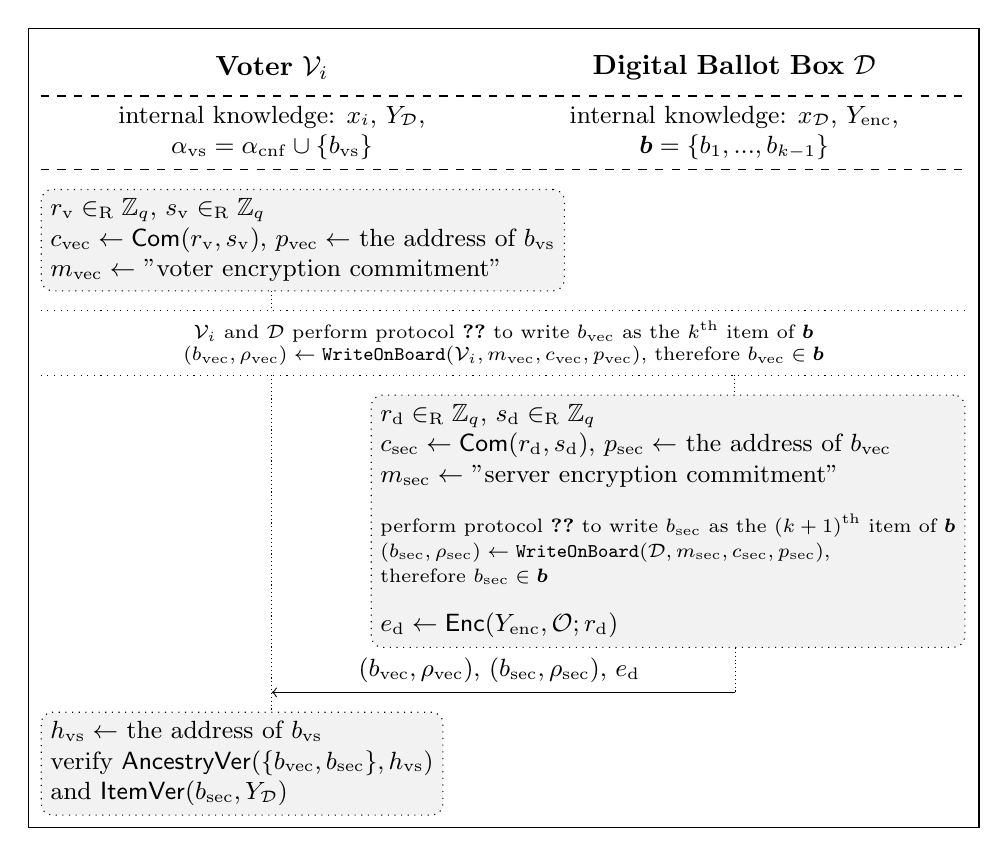
\begin{tikzpicture}[framed, node distance=0,
            % every node/.style={draw}
            ]{
            
        % Actors
        \node[title, above, anchor=north east] (v) {
            \textbf{Voter $\mathcal{V}_i$}};
        \node[title, right=of v] (dbb) {
            \textbf{Digital Ballot Box $\mathcal{D}$}};
        
        % internal knowledge
        \node[ik] at (v.south) (v_ik) {
            internal knowledge: $x_i$, $Y_\mathcal{D}$, \\
            $\alpha_\mathrm{vs} = \alpha_\mathrm{cnf} \cup \{ b_\mathrm{vs} \}$
            };
        \node[ik] at (dbb.south) (dbb_ik) {
            internal knowledge: $x_\mathcal{D}$, $Y_\mathrm{enc}$, \\
            $\boldsymbol{b} = \{ b_1, ..., b_{k-1} \}$
            };
        
        %All content
        \node[block, keep_left, spaced] at (dbb_ik.south -| v.west) (v_1) {
            $r_\mathrm{v} \in_\mathrm{R} \mathbb{Z}_q$, $s_\mathrm{v} \in_\mathrm{R} \mathbb{Z}_q$ \\
            $c_\mathrm{vec} \gets \mathsf{Com}(r_\mathrm{v}, s_\mathrm{v})$, $p_\mathrm{vec} \gets$ the address of $b_\mathrm{vs}$ \\
            $m_\mathrm{vec} \gets$ "voter encryption commitment"
            };
        \node[banner, keep_left, spaced, between={v.west}{dbb.east}] at (v_1.south -| v.west) (b_1) {
            $\mathcal{V}_i$ and $\mathcal{D}$ perform protocol \ref{pro: write on board} to write $b_\mathrm{vec}$ as the $k^\mathrm{th}$ item of $\boldsymbol{b}$ \\
            $(b_\mathrm{vec}, \rho_\mathrm{vec}) \gets \mathtt{WriteOnBoard}(\mathcal{V}_i, m_\mathrm{vec}, c_\mathrm{vec}, p_\mathrm{vec})$, therefore $b_\mathrm{vec} \in \boldsymbol{b}$
            };
        \node[block, keep_right, spaced] at (b_1.south -| dbb.east) (dbb_1) {
            $r_\mathrm{d} \in_\mathrm{R} \mathbb{Z}_q$, $s_\mathrm{d} \in_\mathrm{R} \mathbb{Z}_q$ \\
            $c_\mathrm{sec} \gets \mathsf{Com}(r_\mathrm{d}, s_\mathrm{d})$, $p_\mathrm{sec} \gets$ the address of $b_\mathrm{vec}$ \\
            $m_\mathrm{sec} \gets$ "server encryption commitment" \\ [7pt]
            \scriptsize perform protocol \ref{pro: write on board} to write $b_\mathrm{sec}$ as the $(k+1)^\mathrm{th}$ item of $\boldsymbol{b}$ \\ [-2pt]
            \scriptsize $(b_\mathrm{sec}, \rho_\mathrm{sec}) \gets \mathtt{WriteOnBoard}(\mathcal{D}, m_\mathrm{sec}, c_\mathrm{sec}, p_\mathrm{sec})$, \\[-2pt] 
            \scriptsize therefore $b_\mathrm{sec} \in \boldsymbol{b}$ \\ [7pt]
            $e_\mathrm{d} \gets \mathsf{Enc}(Y_\mathrm{enc}, \mathcal{O}; r_\mathrm{d})$
            };
        \node[arrow, towards_left, between={v.center}{dbb.center}] at (dbb_1.south -| v.center) (a_1) {
            $(b_\mathrm{vec}, \rho_\mathrm{vec})$, $(b_\mathrm{sec}, \rho_\mathrm{sec})$, $e_\mathrm{d}$
            };
        \node[block, keep_left, spaced] at (a_1.south -| v.west) (v_2) {
            $h_\mathrm{vs} \gets $ the address of $b_\mathrm{vs}$ \\
            verify $\mathsf{AncestryVer}(\{ b_\mathrm{vec}, b_\mathrm{sec} \}, h_\mathrm{vs})$ \\
            and $\mathsf{ItemVer}(b_\mathrm{sec}, Y_\mathcal{D})$
            };
        
        % Arrows and lines
        \draw[dashed] (v.south west)--(dbb.south east);    
        \draw[dashed] (dbb_ik.south -| v.west)--(dbb_ik.south -| dbb.east);

        \draw[dotted] (b_1.north west)--(b_1.north east);
        \draw[dotted] (b_1.south west)--(b_1.south east);

        \draw[densely dotted] (v_1.south -| v.center)--(b_1.north -| v.center);
        \draw[densely dotted] (b_1.south -| v.center)--(v_2.north -| v.center);

        \draw[densely dotted] (b_1.south -| dbb.center)--(dbb_1.north -| dbb.center);
        \draw[densely dotted] (dbb_1.south -| a_1.east)--(a_1.south east);
        }
    \end{tikzpicture}
    \caption{Encryption commitments submission protocol}
    \label{fig: encryption commitments submission protocol}
\end{figure}

\begin{figure}[ht]
    \centering
    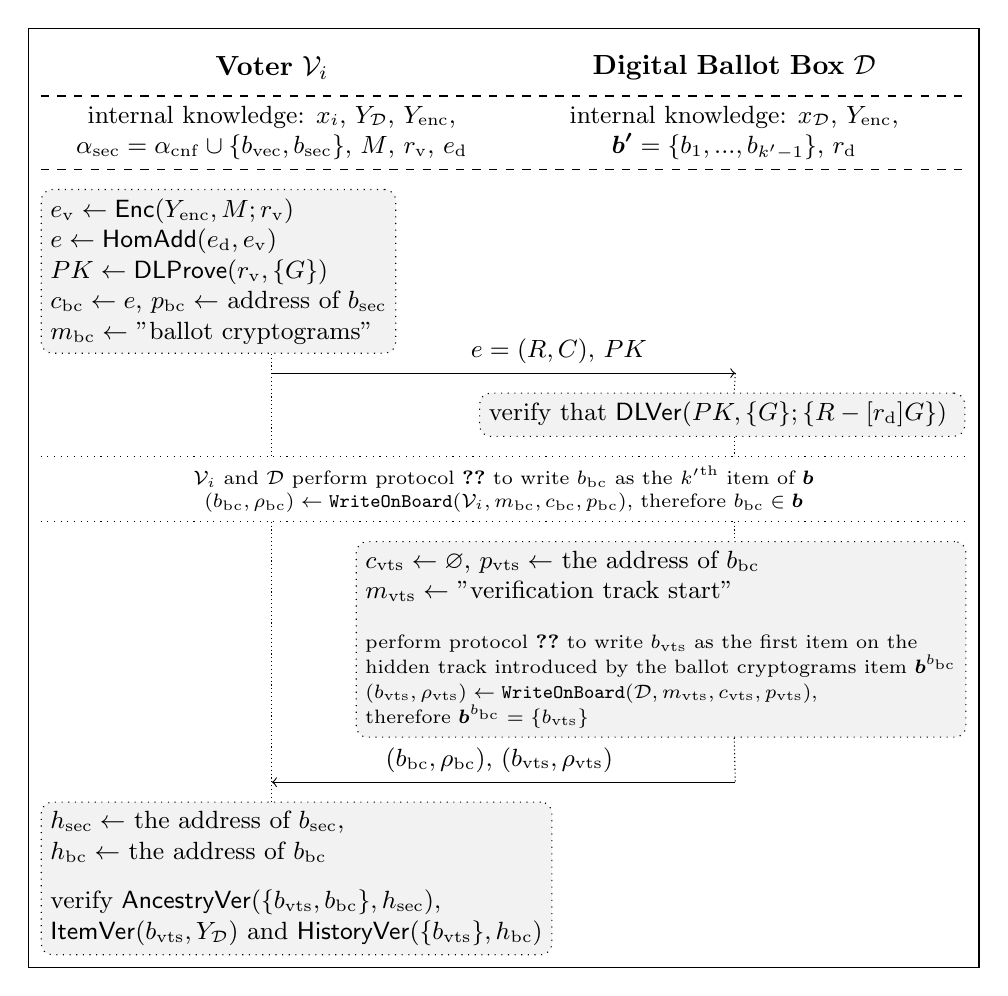
\begin{tikzpicture}[framed,
            node distance=0,
            % every node/.style={draw}
            ]{
            
        % Actors
        \node[title, above, anchor=north east] (v) {
            \textbf{Voter $\mathcal{V}_i$}};
        \node[title, right=of v] (dbb) {
            \textbf{Digital Ballot Box $\mathcal{D}$}};
        
        % internal knowledge
        \node[ik] at (v.south) (v_ik) {
            internal knowledge: $x_i$, $Y_\mathcal{D}$, $Y_\mathrm{enc}$, \\
            $\alpha_\mathrm{sec} = \alpha_\mathrm{cnf} \cup \{ b_\mathrm{vec}, b_\mathrm{sec} \}$, $M$, $r_\mathrm{v}$, $e_\mathrm{d}$
            };
        \node[ik] at (dbb.south) (dbb_ik) {
            internal knowledge: $x_\mathcal{D}$, $Y_\mathrm{enc}$, \\
            $\boldsymbol{b'} = \{ b_1, ..., b_{k'-1} \}$, $r_\mathrm{d}$
            };
        
        %All content
        \node[block, spaced, keep_left] at (v_ik.south -| v.west) (v_1) {
            $e_\mathrm{v} \gets \mathsf{Enc}(Y_\mathrm{enc}, M; r_\mathrm{v})$ \\
            $e \gets \mathsf{HomAdd}(e_\mathrm{d}, e_\mathrm{v})$ \\
            $PK \gets \mathsf{DLProve}(r_\mathrm{v}, \{ G \})$ \\
            $c_\mathrm{bc} \gets e$, $p_\mathrm{bc} \gets$ address of $b_\mathrm{sec}$ \\
            $m_\mathrm{bc} \gets$ "ballot cryptograms"
            };
        \node[arrow, towards_right, immediate, between={v.center}{dbb.center}] at (v_1.south -| v.center) (a_1) {
            \hspace{40pt} $e = (R, C)$, $PK$
            };
        \node[block, keep_right, spaced] at (a_1.south -| dbb.east) (dbb_1) {
            verify that $\mathsf{DLVer}(PK, \{ G \}; \{ R - [r_\mathrm{d}]G \})$
            };
        \node[banner, keep_left, spaced, between={v.west}{dbb.east}] at (dbb_1.south -| v.west) (b_1) {
            $\mathcal{V}_i$ and $\mathcal{D}$ perform protocol \ref{pro: write on board} to write $b_\mathrm{bc}$ as the ${k'}^\mathrm{th}$ item of $\boldsymbol{b}$ \\
            $(b_\mathrm{bc}, \rho_\mathrm{bc}) \gets \mathtt{WriteOnBoard}(\mathcal{V}_i, m_\mathrm{bc}, c_\mathrm{bc}, p_\mathrm{bc})$, therefore $b_\mathrm{bc} \in \boldsymbol{b}$
            };
        \node[block, keep_right, spaced] at (b_1.south east) (dbb_2) {
            $c_\mathrm{vts} \gets \varnothing$, $p_\mathrm{vts} \gets$ the address of $b_\mathrm{bc}$ \\
            $m_\mathrm{vts} \gets$ "verification track start" \\ [7pt]
            \scriptsize perform protocol \ref{pro: write on board} to write $b_\mathrm{vts}$ as the first item on the \\ [-2pt]
            \scriptsize hidden track introduced by the ballot cryptograms item $\boldsymbol{b}^{b_\mathrm{bc}}$ \\ [-2pt]
            \scriptsize $(b_\mathrm{vts}, \rho_\mathrm{vts}) \gets \mathtt{WriteOnBoard}(\mathcal{D}, m_\mathrm{vts}, c_\mathrm{vts}, p_\mathrm{vts})$, \\ [-2pt]
            \scriptsize therefore $\boldsymbol{b}^{b_\mathrm{bc}} = \{ b_\mathrm{vts} \}$
            };
        \node[arrow, towards_left, between={v.center}{dbb.center}] at (dbb_2.south -| v.center) (a_2) {
            $(b_\mathrm{bc}, \rho_\mathrm{bc})$, $(b_\mathrm{vts}, \rho_\mathrm{vts})$
            };
        \node[block, keep_left, spaced] at (a_2.south -| v.west) (v_2) {
            $h_\mathrm{sec} \gets $ the address of $b_\mathrm{sec}$, \\
            $h_\mathrm{bc} \gets $ the address of $b_\mathrm{bc}$ \\ [7pt]
            verify $\mathsf{AncestryVer}(\{ b_\mathrm{vts}, b_\mathrm{bc} \}, h_\mathrm{sec})$, \\
            $\mathsf{ItemVer}(b_\mathrm{vts}, Y_\mathcal{D})$ and $\mathsf{HistoryVer}(\{ b_\mathrm{vts} \}, h_\mathrm{bc})$
            };
        
        % Arrows and lines
        \draw[dashed] (v.south west)--(dbb.south east);    
        \draw[dashed] (dbb_ik.south -| v.west)--(dbb_ik.south -| dbb.east);

        \draw[dotted] (b_1.north west)--(b_1.north east);
        \draw[dotted] (b_1.south west)--(b_1.south east);

        \draw[densely dotted] (v_1.south -| v.center)--(b_1.north -| v.center);
        \draw[densely dotted] (b_1.south -| v.center)--(v_2.north -| v.center);

        \draw[densely dotted] (a_1.south east)--(dbb_1.north -| dbb.center);
        \draw[densely dotted] (dbb_1.south -| dbb.center)--(b_1.north -| dbb.center);
        \draw[densely dotted] (b_1.south -| dbb.center)--(dbb_2.north -| dbb.center);
        \draw[densely dotted] (dbb_2.south -| dbb.center)--(a_2.south east);
        }
    \end{tikzpicture}
    \caption{Encrypted ballot submission protocol}
    \label{fig: encrypted ballot submission protocol}
\end{figure}

The generation process begins by the voting application generating its encryption randomizer $r_\mathrm{v} \in_\mathrm{R} \mathbb{Z}_q$ and computing a commitment to it $c_\mathrm{v} \gets \mathsf{Com}(r_\mathrm{v}, s_\mathrm{v})$ (\cref{alg: com}), where $s_\mathrm{v} \in_\mathrm{R} \mathbb{Z}_q$. Then, the voting application interacts with the digital ballot box in the protocol \ref{pro: write on board} $\mathtt{WriteOnBoard}(\mathcal{V}_i, m_\mathrm{vec}, c_\mathrm{vec}, p_\mathrm{vec})$ in order to append the vote encryption commitment item $b_\mathrm{vec}$ on the board, where $m_\mathrm{vec} =$ "voter encryption commitment", the content $c_\mathrm{vec}$ consists of the commitment $c_\mathrm{v}$ and the parent $p_\mathrm{vec}$ is the address of the voter session item as received in \cref{sec: voter authorization procedure}. Note that before appending the new item, the bulletin board consists of items $\boldsymbol{b} = \{ b_1, ..., b_{k-1} \}$, therefore $b_\mathrm{vec}$ becoming the $k^\mathrm{th}$ item.

After publishing the voter encryption commitment item on the bulletin board, the digital ballot box immediately generates its own set of encryption randomizer $r_\mathrm{d} \in_\mathrm{R} \mathbb{Z}_q$ and commitment $c_\mathrm{d} \gets \mathsf{Com}(r_\mathrm{d}, s_\mathrm{d})$ (\cref{alg: com}), where $s_\mathrm{d} \in_\mathrm{R} \mathbb{Z}_q$. Then, it self writes a server encryption commitment item $b_\mathrm{sec}$ on the board by running protocol \ref{pro: write on board} $\mathtt{WriteOnBoard}(\mathcal{D}, m_\mathrm{sec}, c_\mathrm{sec}, p_\mathrm{sec})$, where $m_\mathrm{sec} =$ "server encryption commitment", the content $c_\mathrm{sec}$ consists of its commitment $c_\mathrm{d}$ and the parrent $p_\mathrm{sec}$ is the address of the voter encryption commitment item $b_\mathrm{vec}$.

Next, the digital ballot box returns to the voting application both items $b_\mathrm{vec}$ and $b_\mathrm{sec}$ together with their respective receipts, according to the protocol \ref{pro: write on board} described in \cref{sec: writing on the bulletin board} and the empty cryptogram $e_\mathrm{d}$, i.e. the encryption of the neutral point $\mathcal{O}$ using the encryption randomizer $r_\mathrm{d}$. The voting application performs the validation of the board items $b_\mathrm{vec}$ and $b_\mathrm{sec}$ according to the protocol \ref{pro: write on board} and continues if successful.

After both parties have published their encryption commitment items, as presented in \cref{fig: encrypted ballot submission protocol}, the voting application encrypts the voter's encoded vote $M$ (as constructed in \cref{sec: mapping vote options on the elliptic curve}) by computing $e_\mathrm{v} \gets \mathsf{Enc}(Y_\mathrm{enc}, M; r_\mathrm{v})$ (\cref{alg: enc}). This gets further combined with the empty cryptogram received from the digital ballot box, to produce the voter's final ballot cryptogram $e \gets \mathsf{HomAdd}(e_\mathrm{v}, e_\mathrm{d})$ (\cref{alg: hom add}). The voting application also computes a proof of correct encryption $PK \gets \mathsf{DLProve}(r_\mathrm{v})$ (\cref{alg: dl prove}) that confirms the fact that the empty cryptogram $e_\mathrm{d}$ has been used in computation of the final ballot cryptogram $e$.

Finally, the voting application interacts with the digital ballot box in the protocol $\mathtt{WriteOnBoard}(\mathcal{V}_i, m_\mathrm{bc}, c_\mathrm{bc}, p_\mathrm{bc})$ (protocol \ref{pro: write on board}) in order to append the ballot cryptogram item $b_\mathrm{bc}$ on the board, where $m_\mathrm{bc} =$ "ballot cryptograms", the content $c_\mathrm{bc}$ consists of the cryptogram $e$ and the parrent $p_\mathrm{bc}$ is the address of the server encryption commitment item $b_\mathrm{sec}$. Note that this time, the bulletin board consists of items $\boldsymbol{b'} = \{ b_1, ..., b_{k'-1} \}$, where $k' \geq k$ as more items could have been appended by other voters in between protocols from \cref{fig: encryption commitments submission protocol} and \cref{fig: encrypted ballot submission protocol}, therefore $b_\mathrm{bc}$ becoming the ${k'}^\mathrm{th}$ item.

Additionally, the voting application submits the proof $PK$ to the digitla ballot box, which performs protocol \ref{pro: write on board} if $\mathsf{DLVer}(PK, \{ G \}, \{ R - [r_\mathrm{d}]G \})$ (\cref{alg: dl ver}) succeeds, where the content of the item  $c_\mathrm{bc}$ consists of $e = (R, C)$.

After publishing the ballot cryptograms item on the bulletin board, the digital ballot box immediately self writes a verification track start item $b_\mathrm{vts}$ on the hidden track of the bulletin board $\boldsymbol{b}^{b_\mathrm{bc}}$ by running $\mathtt{WriteOnBoard}(\mathcal{D}, m_\mathrm{vts}, c_\mathrm{vts}, p_\mathrm{vts})$ (protocol \ref{pro: write on board}), where $m_\mathrm{vts} =$ "verification track start", the content $c_\mathrm{sec}$ is empty and the parent $p_\mathrm{vts}$ is the address of the ballot cryptogram item $b_\mathrm{bc}$. Note that at this point, the hidden track contains $\boldsymbol{b}^{b_\mathrm{bc}} = \{ b_\mathrm{vts} \}$.

Next, the digital ballot box returns to the voting application both items $b_\mathrm{bc}$ and $b_\mathrm{vts}$ together with their respective receipts, according to the protocol \ref{pro: write on board}. The voting application performs the validation of the two board items according to the protocol \ref{pro: write on board}. In addition, it checks that the verification track start item is the only item on the hidden track by $\mathsf{HistoryVer}(\{ b_\mathrm{vts} \}, h_\mathrm{bc})$ (\cref{alg: history ver}), where $h_\mathrm{bc}$ is the address of the ballot cryptograms item.

Note that, the cryptogram $e$ is actually equivalent to $\mathsf{Enc}(Y_\mathrm{enc}, M; r)$, where $r = r_\mathrm{v} + r_\mathrm{d}$. Both the voter and the digital ballot box know part of the randomizer value, $r_\mathrm{v}$ and $r_\mathrm{d}$ respectively, but neither of them knows the combined value $r$.


\subsubsection{Challenging a vote cryptogram} \label{sec: challenging a vote cryptogram}
After encrypting a ballot, the voter $\mathcal{V}_i$ can choose whether to test or cast it. To perform the testing process of an encrypted ballot, the voter needs to interact with the \textit{external verifier} that will perform all the testing operations on behalf of the voter, according to the data published on the bulletin board. At the end of the testing process, the voter will be presented with the vote choice(s) that were encoded in the encrypted ballot. When doing the testing procedure, the encrypted ballot that is being tested gets spoiled. Therefore, the voter needs to redo the vote cryptogram generation process from \cref{sec: vote cryptogram generation process} to get a new encrypted ballot, which the voter has to choose again whether to test or to cast. This process can be repeated until the voter trusts the legitimacy of the next encrypted ballot generated by the voting application. The protocol is inspired from \cite{Benaloh06}.

The first part of the protocol (\cref{fig: external verifier setup protocol}) establishes a trusted connection amongst the voting application and the external verifier over the bulletin board. The voter inputs into the external verifier the address of the verification track start item $b_\mathrm{vts}$, which queries the digital ballot box for the item at that address and its ancestry. The digital ballot box returns $\alpha_\mathrm{vts} = \alpha_\mathrm{cnf} \cup \{ b_\mathrm{vs}, b_\mathrm{vec}, b_\mathrm{sec}, b_\mathrm{bc}, b_\mathrm{vts} \}$, which consists of all the configuration items (e.g. the genesis item, election configuration items, contest configuration items, etc.) plus all the voting items that are relevant to voter $\mathcal{V}_i$. Notice that all configuration and voting items are on the public bulletin board (i.e. $\alpha_\mathrm{cnf}, b_\mathrm{vs}, b_\mathrm{vec}, b_\mathrm{sec}, b_\mathrm{bc} \in \boldsymbol{b}$), except the verification track start item $b_\mathrm{vts}$ which exists on the hidden track $\boldsymbol{b}^{b_\mathrm{bc}}$ that has been spawned by the ballot cryptograms item $b_\mathrm{bc}$.

The external verifier validates the list by running $\mathsf{AncestryVer}(\alpha_\mathrm{vts}, \varnothing)$ (\cref{alg: ancestry ver}), therefore checking that $\alpha_\mathrm{vts}$ has a consistent ancestry all the way through the genesis item, with has no parent, therefore the parent of the entire ancestry is null or $\varnothing$. The external verifier also checks the integrity of every item by $\mathsf{ItemVer}(b_j, Y_\mathcal{W})$ (\cref{alg: item ver}), where $b_j \in \alpha_\mathrm{vts}$ and $Y_\mathcal{W}$ is the public key of the respective writer, according to the rules from \cref{app: bulletin board item types}. Note that the set of writers, as presented in \cref{sec: public bulletin board}, consists of the voter $\mathcal{V}_i$, the digital ballot box $\mathcal{D}$, the election administrator $\mathcal{E}$ and the voter authorizer $\mathcal{A}$. The external verifier can extract the voter's public key $Y_i$ from the voter session item $b_\mathrm{vs}$ and the other public keys $Y_\mathcal{D}$, $Y_\mathcal{E}$ and $Y_\mathcal{A}$ from the configuration items. If valid, the external verifier notifies the voter that the ballot was successfully found.

Then, the voter chooses to test the encryption of the ballot, so the voting application interacts with the digital ballot box in $\mathtt{WriteOnBoard}(\mathcal{V}_i, m_\mathrm{sr}, c_\mathrm{sr}, p_\mathrm{sr})$ (protocol \ref{pro: write on board}) to append the spoil request item $b_\mathrm{sr}$ on the board, where $m_\mathrm{sr} = $ "spoil request", the content $c_\mathrm{sr}$ is empty and the parent $p_\mathrm{sr}$ is the address of the ballot cryptograms item $b_\mathrm{bc}$.

After publishing the spoil request item $b_\mathrm{sr}$, the digital ballot box sends the new item also to the external verifier, which verifies its integrity $\mathsf{ItemVer}(b_\mathrm{sr}, Y_i)$ (\cref{alg: item ver}) and that it is consistent with the ancestry $\mathsf{AncestryVer}(\{ b_\mathrm{sr} \}, h_\mathrm{bc})$ (\cref{alg: ancestry ver}), where $h_\mathrm{bc}$ is the address of the ballot cryptograms item $b_\mathrm{bc}$. If valid, the external verifier generates its own key pair $(x_\mathcal{X}, Y_\mathcal{X}) \gets \mathsf{KeyGen}()$ (\cref{alg: key gen}) and interacts with digital ballot box in $\mathtt{WriteOnBoard}(\mathcal{X}, m_\mathrm{v}, c_\mathrm{v}, p_\mathrm{v})$ (protocol \ref{pro: write on board}) to write a verifier item $b_\mathrm{v}$ on the hidden track, where $m_\mathrm{v} =$ "verifier", the content $c_\mathrm{v}$ contains the external verifier's public key $Y_\mathcal{X}$ and the parent $p_\mathrm{v}$ is the address of the spoil request item $b_\mathrm{sr}$. Note that the verifier item $b_\mathrm{v}$ is appended on the hidden track introduces by the ballot cryptograms item $b_\mathrm{bc}$. Therefore, at the end of this step, the hidden track consists of $\boldsymbol{b}^{b_\mathrm{bc}} = \{ b_\mathrm{vts}, b_\mathrm{v} \}$. From this point on, the external verifier represents indentity $\mathcal{X}$ on the hidden track $\boldsymbol{b}^{b_\mathrm{bc}}$.

The protocol continues with \cref{fig: commitment opening submission protocol} where the external verifier returns to the voter with the address of the verifier item $h_\mathrm{v}$. The voter also receives the verifier item $b_\mathrm{v}$ from the digital ballot box. The voter checks the integrity of the item $\mathsf{ItemVer}(b_\mathrm{v}, Y_\mathcal{X})$ (\cref{alg: item ver}) and that it is consistent with the ancestry $\mathsf{AncestryVer}(\{ b_\mathrm{v} \}, h_\mathrm{vts})$ (\cref{alg: ancestry ver}), where $Y_\mathcal{X}$ is extracted from the content of the verifier item and $h_\mathrm{vts}$ is the address of the verification track start item. Then the voter checks that the address received from the external verifier is consistent with the verifier item received from the digital ballot box. If valid, the voter managed to establish a trusted connection with the external verifier over the bulletin board, therefore the protocol can continue.

Next, both the voter and the digital ballot box collaborate to deliver to the external verifier, in a secure manner, their encryption randomizer $r_\mathrm{v}$ and $r_\mathrm{s}$ respectively, as generated in \cref{sec: vote cryptogram generation process}. The external verifier will use them to decrypt the voter's ballot cryptograms and present the vote choices to the voter for assessment.

This is achieved by the voter encrypting (using standard symmetric key encryption) the randomizer and the commitment opening $d_\mathrm{v} \gets \mathsf{SymEnc}(k_\mathrm{v}, r_\mathrm{v} || s_\mathrm{v})$ (\cref{alg: sym enc}), where $k_\mathrm{v}$ is a derived symmetric key based on Diffie-Hellman key exchange mechanism between the voter and the external verifier, i.e. $k_\mathrm{v} \gets \mathsf{DerSymKey}(x_i, Y_\mathcal{X})$ (\cref{alg: der sym key}). Then, the voter interacts with the digital ballot box to write the voter commitment opening item $b_\mathrm{vco}$ on the hidden track $\mathtt{WriteOnBoard}(\mathcal{V}_i, m_\mathrm{vco}, c_\mathrm{vco}, p_\mathrm{vco})$ (protocol \ref{pro: write on board}), where $m_\mathrm{vco} = $ "voter commitment opening", content $c_\mathrm{vco}$ consists of the encryption $d_\mathrm{v}$ and the parent $p_\mathrm{v}$ is the address of the verifier item $b_\mathrm{v}$.

After publishing the voter commitment opening item, the digital ballot box immediately computes its own encryption of the randomizer and commitment opening $d_\mathrm{d}$ using the same strategy as the voter in the previous paragraph. Then, it self writes a server commitment opening item $b_\mathrm{sco}$ on the board by running $\mathtt{WriteOnBoard}(\mathcal{D}, m_\mathrm{sco}, c_\mathrm{sco}, p_\mathrm{sco})$ (protocol \ref{pro: write on board}), where $m_\mathrm{sco} =$ "server commitment opening", the content $c_\mathrm{sec}$ consists of the encryption $d_\mathrm{d}$ and the parrent $p_\mathrm{sco}$ is the address of the voter commitment opening item $b_\mathrm{vco}$. 

Then (\cref{fig: unpacking the encrypted ballot protocol}), the external verifier is notified about both commitment opening items, which verifies the integrity of them and that they are consistent with the previous ancestry. If valid, it decrypts (using standard symmetric key decryption) both commitment openings, of the voter $(r_\mathrm{v}, s_\mathrm{v}) \gets \mathsf{SymDec}(k_\mathrm{v}, d_\mathrm{v})$ (\cref{alg: sym dec}) and of the digital ballot box $(r_\mathrm{d}, s_\mathrm{d}) \gets \mathsf{SymDec}(k_\mathrm{d}, d_\mathrm{d})$, where the encryptions $d_\mathrm{v}$ and $d_\mathrm{d}$ are extracted from the content of the voter and of the server commitment opening items respectively, and the symmetric keys $k_\mathrm{v}$ and $k_\mathrm{d}$ are computed based on the Diffie-Hellman key exchange mechanism between the external verifier and the voter or the digital ballot box respectively.

Next, the external verifier checks whether the commitment openings are consistent with the commitments that were published in \cref{sec: vote cryptogram generation process}, i.e. verification of the voter commitment $\mathsf{ComVer}(c_\mathrm{v}, r_\mathrm{v}, s_\mathrm{v})$ (\cref{alg: com ver}) and of the server commitment $\mathsf{ComVer}(c_\mathrm{d}, r_\mathrm{d}, s_\mathrm{d})$, where commitments $c_\mathrm{v}$ and $c_\mathrm{d}$ are extracted from the voter and server encryption commitment items respectively. If commitments are validated, the external verifier proceeds to the unpacking of the cryptogram $e$, which is extracted from the ballot cryptograms items $b_\mathrm{bc}$. If any of the validations fail, the external verifier informs the voter about the failure.

The external verifier unpacks the vote $V'$ by decrypting a variant of the cryptogram $e = (R, C)$, where point $R$ is substituted by the encryption key $Y_\mathrm{enc}$, such that it can be decrypted by the randomizer $r_\mathrm{v} + r_\mathrm{d}$ instead of the decryption key. Note that, the encryption key $Y_\mathrm{enc}$ can be extracted from the threshold configuration item, which is part of $\alpha_\mathrm{cnf}$. Formally, $V' \gets \mathsf{Dec}(r_\mathrm{v} + r_\mathrm{d}, e')$ (\cref{alg: dec}), where $e' \gets (Y_\mathrm{enc}, C)$.

Finally, the external verifier presents to the voter, the plain text vote $V'$, which can compare to the original vote choice $V$, as computed in \cref{sec: mapping vote options on the elliptic curve}. Note that $V'$ can even be decoded into a human readable presentation of the vote choices by converting it to bytes $\mathsf{Point2Bytes}(V')$ (\cref{alg: point to bytes}) and then into a plaintext vote according to the configuration from $\alpha_\mathrm{cnf}$. If the vote matches, then the voter is assured that the voting application behaved correctly (i.e. it encrypted a genuine vote). Otherwise, the voter has evidence that the voting application has misbehaved during the process and should act accordingly.

\clearpage
\begin{landscape}
\begin{figure}[ht]
    \centering
    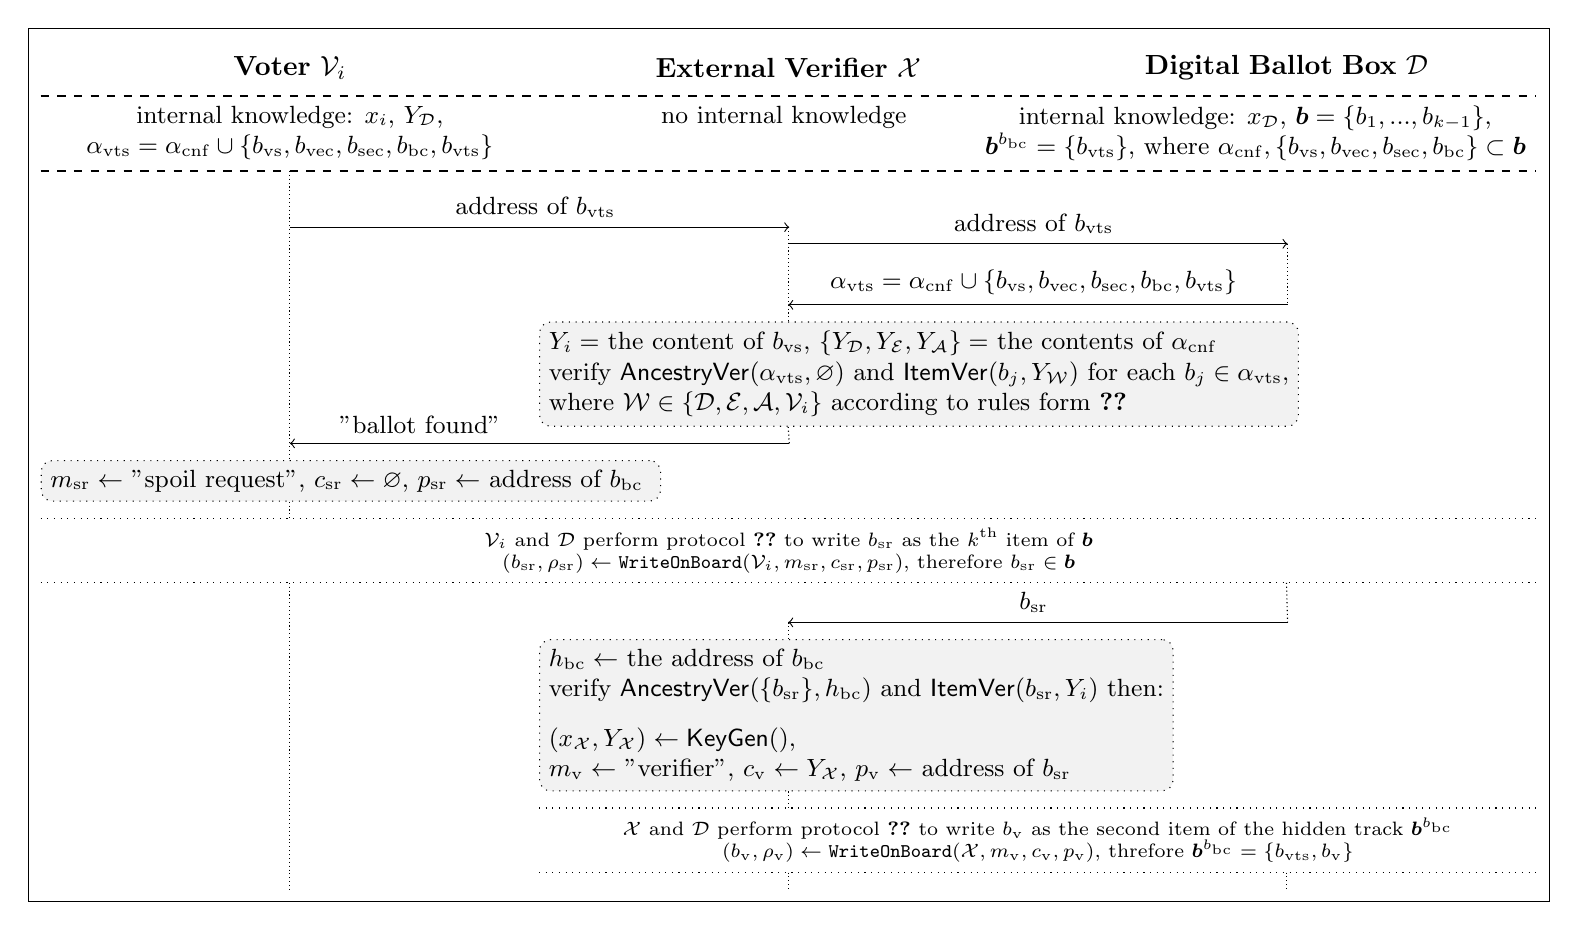
\begin{tikzpicture}[framed, node distance=0,
            spaced/.style={yshift=-6},
            % every node/.style={draw},
            ]{
        
        % Actors
        \node[title_3, above, anchor=north east] (v) {
            \textbf{Voter $\mathcal{V}_i$}};
        \node[title_3, right=of v] (ev) {
            \textbf{External Verifier $\mathcal{X}$}};
        \node[title_3, right=of ev] (dbb) {
            \textbf{Digital Ballot Box $\mathcal{D}$}};

        % internal knowledge
        \node[ik] at (v.south) (v_ik) {
            internal knowledge: $x_i$, $Y_\mathcal{D}$, \\
            $\alpha_\mathrm{vts} = \alpha_\mathrm{cnf} \cup \{ b_\mathrm{vs}, b_\mathrm{vec}, b_\mathrm{sec}, b_\mathrm{bc}, b_\mathrm{vts} \}$
            };
        \node[ik] at (ev.south) (ev_ik) {
            no internal knowledge
            };
        \node[ik, keep_right] at (dbb.south east) (dbb_ik) {
            internal knowledge: $x_\mathcal{D}$, $\boldsymbol{b} = \{ b_1, ..., b_{k-1} \}$, \\
            $\boldsymbol{b}^{b_\mathrm{bc}} = \{ b_\mathrm{vts} \}$, where $\alpha_\mathrm{cnf}, \{ b_\mathrm{vs}, b_\mathrm{vec}, b_\mathrm{sec}, b_\mathrm{bc} \} \subset \boldsymbol{b}$
            };
        
        % All content
        \node[arrow, towards_right, spaced, between={v.center}{ev.center}] at (dbb_ik.south -| v.center) (a_1) {
            address of $b_\mathrm{vts}$
            };
        \node[arrow, towards_right, immediate, between={ev.center}{dbb.center}] at (a_1.south -| ev.center) (a_2) {
            address of $b_\mathrm{vts}$
            };
        \node[arrow, towards_left, spaced, between={ev.center}{dbb.center}] at (a_2.south -| ev.center) (a_3) {
            $\alpha_\mathrm{vts} = \alpha_\mathrm{cnf} \cup \{ b_\mathrm{vs}, b_\mathrm{vec}, b_\mathrm{sec}, b_\mathrm{bc}, b_\mathrm{vts} \}$
            };
        \node[block, keep_left, spaced] at (a_3.south -| ev.west) (ev_1) {
            $Y_i = $ the content of $b_\mathrm{vs}$, $\{ Y_\mathcal{D}, Y_\mathcal{E}, Y_\mathcal{A} \} = $ the contents of $\alpha_\mathrm{cnf}$ \\
            verify $\mathsf{AncestryVer}(\alpha_\mathrm{vts}, \varnothing)$ and $\mathsf{ItemVer}(b_j, Y_\mathcal{W})$ for each $b_j \in \alpha_\mathrm{vts}$, \\
            where $\mathcal{W} \in \{ \mathcal{D}, \mathcal{E}, \mathcal{A}, \mathcal{V}_i \}$ according to rules form \cref{app: bulletin board item types}
            };
        \node[arrow, towards_left, immediate, between={v.center}{ev.center}] at (ev_1.south -| v.center) (a_4) {
            "ballot found" \hspace{80pt}
            };
        \node[block, keep_left, spaced] at (a_4.south -| v.west) (v_1) {
            $m_\mathrm{sr} \gets $ "spoil request", $c_\mathrm{sr} \gets \varnothing$, $p_\mathrm{sr} \gets$ address of $b_\mathrm{bc}$
            };
        \node[banner, keep_left, spaced, between={v.west}{dbb.east}] at (v_1.south -| v.west) (b_1) {
            $\mathcal{V}_i$ and $\mathcal{D}$ perform protocol \ref{pro: write on board} to write $b_\mathrm{sr}$ as the $k^\mathrm{th}$ item of $\boldsymbol{b}$ \\
            $(b_\mathrm{sr}, \rho_\mathrm{sr}) \gets \mathtt{WriteOnBoard}(\mathcal{V}_i, m_\mathrm{sr}, c_\mathrm{sr}, p_\mathrm{sr})$, therefore $b_\mathrm{sr} \in \boldsymbol{b}$
            };
        \node[arrow, towards_left, between={ev.center}{dbb.center}] at (b_1.south -| ev.center) (a_5) {
            $b_\mathrm{sr}$
            };
        \node[block, keep_left, spaced] at (a_5.south -| ev.west) (ev_2) {
            $h_\mathrm{bc} \gets$ the address of $b_\mathrm{bc}$ \\
            verify $\mathsf{AncestryVer}(\{ b_\mathrm{sr} \}, h_\mathrm{bc})$ and $\mathsf{ItemVer}(b_\mathrm{sr}, Y_i)$ then: \\ [7pt]

            $(x_\mathcal{X}, Y_\mathcal{X}) \gets \mathsf{KeyGen}()$, \\
            $m_\mathrm{v} \gets$ "verifier", $c_\mathrm{v} \gets Y_\mathcal{X}$, $p_\mathrm{v} \gets$ address of $b_\mathrm{sr}$
            };
        \node[banner, keep_left, spaced, between={ev.west}{dbb.east}] at (ev_2.south -| ev.west) (b_2) {
            $\mathcal{X}$ and $\mathcal{D}$ perform protocol \ref{pro: write on board} to write $b_\mathrm{v}$ as the second item of the hidden track $\boldsymbol{b}^{b_\mathrm{bc}}$ \\
            $(b_\mathrm{v}, \rho_\mathrm{v}) \gets \mathtt{WriteOnBoard}(\mathcal{X}, m_\mathrm{v}, c_\mathrm{v}, p_\mathrm{v})$, threfore $\boldsymbol{b}^{b_\mathrm{bc}} = \{ b_\mathrm{vts}, b_\mathrm{v} \}$
            };
        \node[immediate] at (b_2.south) (bottom){};
        
        % Arrows and lines
        \draw[dashed] (v.south west)--(dbb.south east);    
        \draw[dashed] (dbb_ik.south -| v.west)--(dbb_ik.south east);

        \draw[dotted] (b_1.north west)--(b_1.north east);
        \draw[dotted] (b_1.south west)--(b_1.south east);
        \draw[dotted] (b_2.north west)--(b_2.north east);
        \draw[dotted] (b_2.south west)--(b_2.south east);
        
        \draw[densely dotted] (dbb_ik.south -| v.center)--(v_1.north -| v.center);
        \draw[densely dotted] (v_1.south -| v.center)--(b_1.north -| v.center);
        \draw[densely dotted] (b_1.south -| v.center)--(bottom.south -| v.center);
        
        \draw[densely dotted] (a_1.south -| ev.center)--(ev_1.north -| ev.center);
        \draw[densely dotted] (ev_1.south -| ev.center)--(a_4.south east);
        \draw[densely dotted] (a_5.south west)--(ev_2.north -| ev.center);
        \draw[densely dotted] (ev_2.south -| ev.center)--(b_2.north -| ev.center);
        \draw[densely dotted] (b_2.south -| ev.center)--(bottom.south -| ev.center);
        
        \draw[densely dotted] (a_2.south east)--(a_3.south east);
        \draw[densely dotted] (b_1.south -| dbb.center)--(a_5.south east);
        \draw[densely dotted] (b_2.south -| dbb.center)--(bottom.south -| dbb.center);
        }
    \end{tikzpicture}
    \caption{External verifier setup protocol}
    \label{fig: external verifier setup protocol}
\end{figure}

\begin{figure}[ht]
    \centering
    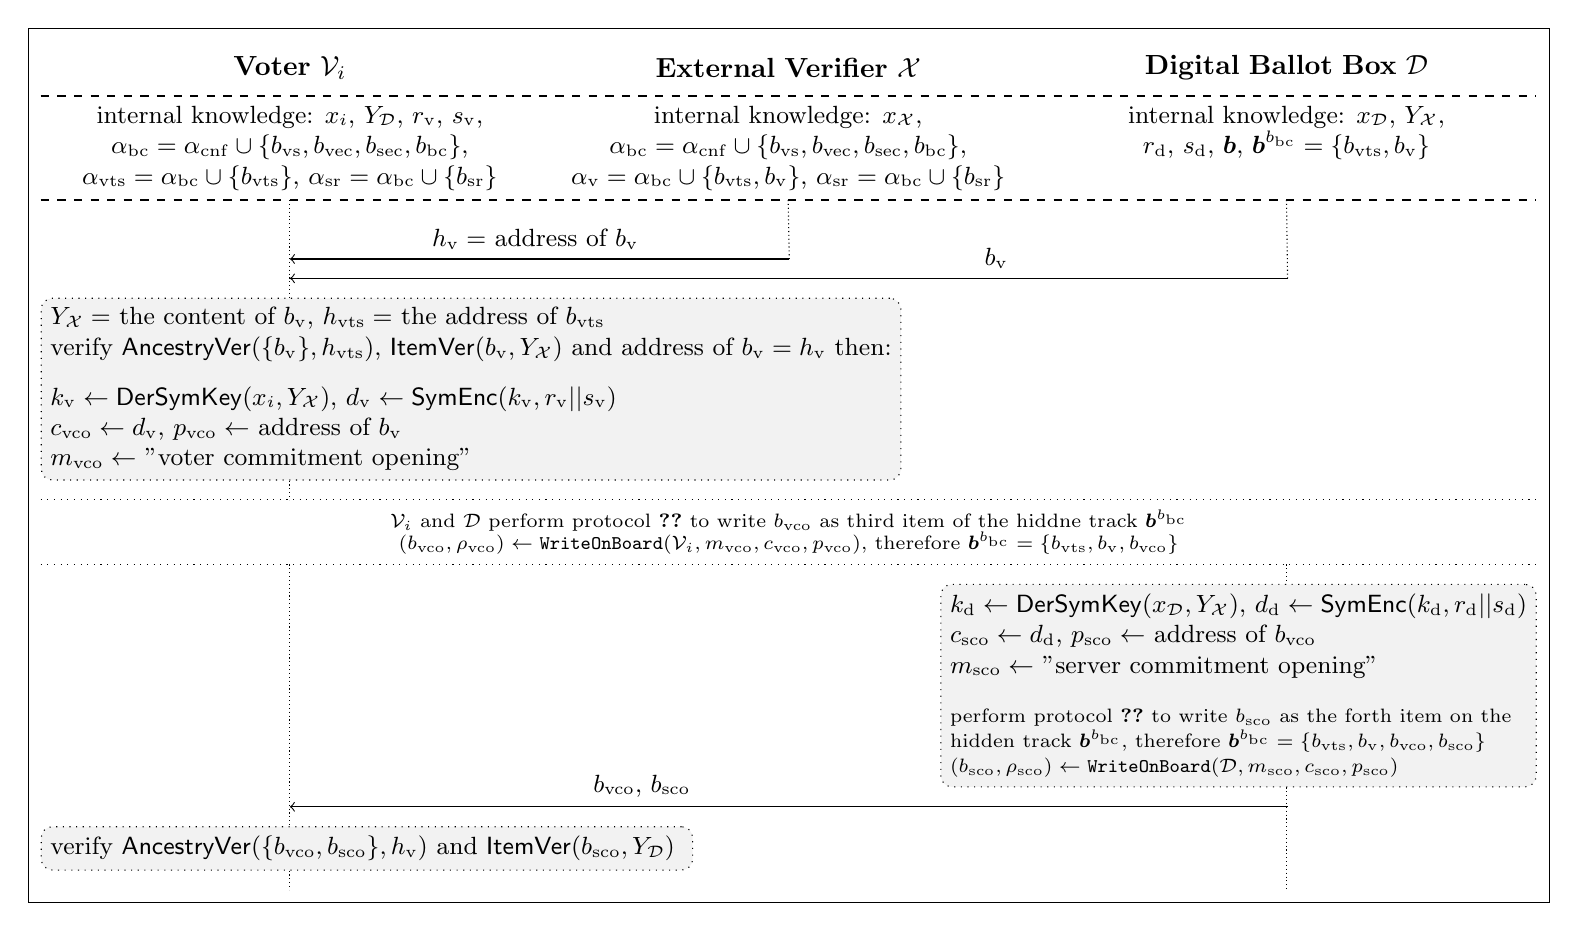
\begin{tikzpicture}[framed, node distance=0,
            % every node/.style={draw},
            ]{
        
        % Actors
        \node[title_3, above, anchor=north east] (v) {
            \textbf{Voter $\mathcal{V}_i$}};
        \node[title_3, right=of v] (ev) {
            \textbf{External Verifier $\mathcal{X}$}};
        \node[title_3, right=of ev] (dbb) {
            \textbf{Digital Ballot Box $\mathcal{D}$}};
        
        % internal knowledge
        \node[ik] at (v.south) (v_ik) {
            internal knowledge: $x_i$, $Y_\mathcal{D}$, $r_\mathrm{v}$, $s_\mathrm{v}$, \\
            $\alpha_\mathrm{bc} = \alpha_\mathrm{cnf} \cup \{ b_\mathrm{vs}, b_\mathrm{vec}, b_\mathrm{sec}, b_\mathrm{bc} \}$, \\
            $\alpha_\mathrm{vts} = \alpha_\mathrm{bc} \cup \{ b_\mathrm{vts} \}$, $\alpha_\mathrm{sr} = \alpha_\mathrm{bc} \cup \{ b_\mathrm{sr} \}$
            };
        \node[ik] at (ev.south) (ev_ik) {
            internal knowledge: $x_\mathcal{X}$, \\
            $\alpha_\mathrm{bc} = \alpha_\mathrm{cnf} \cup \{ b_\mathrm{vs}, b_\mathrm{vec}, b_\mathrm{sec}, b_\mathrm{bc} \}$, \\
            $\alpha_\mathrm{v} = \alpha_\mathrm{bc} \cup \{ b_\mathrm{vts}, b_\mathrm{v} \}$, $\alpha_\mathrm{sr} = \alpha_\mathrm{bc} \cup \{ b_\mathrm{sr} \}$
            };
        \node[ik] at (dbb.south) (dbb_ik) {
            internal knowledge: $x_\mathcal{D}$, $Y_\mathcal{X}$, \\
            $r_\mathrm{d}$, $s_\mathrm{d}$, $\boldsymbol{b}$, $\boldsymbol{b}^{b_\mathrm{bc}} = \{ b_\mathrm{vts}, b_\mathrm{v} \}$
            };
        
        % All content
        \node[arrow, towards_left, spaced, between={v.center}{ev.center}] at (v_ik.south -| v.center) (a_1) {
            $h_\mathrm{v} = $ address of $b_\mathrm{v}$
            };
        \node[arrow, towards_left, immediate, between={v.center}{dbb.center}] at (a_1.south -| v.center) (a_2) {
            \hspace{150pt} $b_\mathrm{v}$
            };
        \node[block, keep_left, spaced] at (a_2.south -| v.west) (v_1) {
            $Y_\mathcal{X} = $ the content of $b_\mathrm{v}$, $h_\mathrm{vts} = $ the address of $b_\mathrm{vts}$ \\
            verify $\mathsf{AncestryVer}(\{ b_\mathrm{v} \}, h_\mathrm{vts})$, $\mathsf{ItemVer}(b_\mathrm{v}, Y_\mathcal{X})$ and address of $b_\mathrm{v} = h_\mathrm{v}$ then: \\ [7pt]
            $k_\mathrm{v} \gets \mathsf{DerSymKey}(x_i, Y_\mathcal{X})$, $d_\mathrm{v} \gets \mathsf{SymEnc}(k_\mathrm{v}, r_\mathrm{v} || s_\mathrm{v})$ \\
            $c_\mathrm{vco} \gets d_\mathrm{v}$, $p_\mathrm{vco} \gets$ address of $b_\mathrm{v}$ \\
            $m_\mathrm{vco} \gets$ "voter commitment opening"
            };
        \node[banner, keep_left, spaced, between={v.west}{dbb.east}] at (v_1.south -| v.west) (b_1) {
            $\mathcal{V}_i$ and $\mathcal{D}$ perform protocol \ref{pro: write on board} to write $b_\mathrm{vco}$ as third item of the hiddne track $\boldsymbol{b}^{b_\mathrm{bc}}$ \\
            $(b_\mathrm{vco}, \rho_\mathrm{vco}) \gets \mathtt{WriteOnBoard}(\mathcal{V}_i, m_\mathrm{vco}, c_\mathrm{vco}, p_\mathrm{vco})$, therefore $\boldsymbol{b}^{b_\mathrm{bc}} = \{ b_\mathrm{vts}, b_\mathrm{v}, b_\mathrm{vco} \}$
            };
        \node[block, keep_right, spaced] at (b_1.south east) (dbb_1) {
            $k_\mathrm{d} \gets \mathsf{DerSymKey}(x_\mathcal{D}, Y_\mathcal{X})$, $d_\mathrm{d} \gets \mathsf{SymEnc}(k_\mathrm{d}, r_\mathrm{d} || s_\mathrm{d})$ \\
            $c_\mathrm{sco} \gets d_\mathrm{d}$, $p_\mathrm{sco} \gets$ address of $b_\mathrm{vco}$ \\
            $m_\mathrm{sco} \gets$ "server commitment opening" \\ [7pt]
            \scriptsize perform protocol \ref{pro: write on board} to write $b_\mathrm{sco}$ as the forth item on the \\ [-2pt]
            \scriptsize hidden track $\boldsymbol{b}^{b_\mathrm{bc}}$, therefore $\boldsymbol{b}^{b_\mathrm{bc}} = \{ b_\mathrm{vts}, b_\mathrm{v}, b_\mathrm{vco}, b_\mathrm{sco} \}$ \\ [-2pt]
            \scriptsize $(b_\mathrm{sco}, \rho_\mathrm{sco}) \gets \mathtt{WriteOnBoard}(\mathcal{D}, m_\mathrm{sco}, c_\mathrm{sco}, p_\mathrm{sco})$
            };
        \node[arrow, towards_left, immediate, between={v.center}{dbb.center}] at (dbb_1.south -| v.center) (a_3) {
            $b_\mathrm{vco}$, $b_\mathrm{sco}$ \hspace{100pt}
            };
        \node[block, keep_left, spaced] at (a_3.south -| v.west) (v_2) {
            verify $\mathsf{AncestryVer}(\{ b_\mathrm{vco}, b_\mathrm{sco} \}, h_\mathrm{v})$ and $\mathsf{ItemVer}(b_\mathrm{sco}, Y_\mathcal{D})$
            };
        \node[immediate] at (v_2.south) (bottom){};
        
        % Arrows and lines
        \draw[dashed] (v.south west)--(dbb.south east);    
        \draw[dashed] (v_ik.south -| v.west)--(v_ik.south -| dbb.east);

        \draw[dotted] (b_1.north west)--(b_1.north east);
        \draw[dotted] (b_1.south west)--(b_1.south east);
        
        \draw[densely dotted] (v_ik.south -| v.center)--(v_1.north -| v.center);
        \draw[densely dotted] (v_1.south -| v.center)--(b_1.north -| v.center);
        \draw[densely dotted] (b_1.south -| v.center)--(v_2.north -| v.center);
        \draw[densely dotted] (v_2.south -| v.center)--(bottom.south -| v.center);
        
        \draw[densely dotted] (v_ik.south -| ev.center)--(a_1.south east);
        
        \draw[densely dotted] (v_ik.south -| dbb.center)--(a_2.south east);
        \draw[densely dotted] (b_1.south -| dbb.center)--(dbb_1.north -| dbb.center);
        \draw[densely dotted] (dbb_1.south -| dbb.center)--(bottom.south -| dbb.center);
        }
    \end{tikzpicture}
    \caption{Commitment opening submission protocol}
    \label{fig: commitment opening submission protocol}
\end{figure}

\clearpage
\begin{figure}[ht]
    \centering
    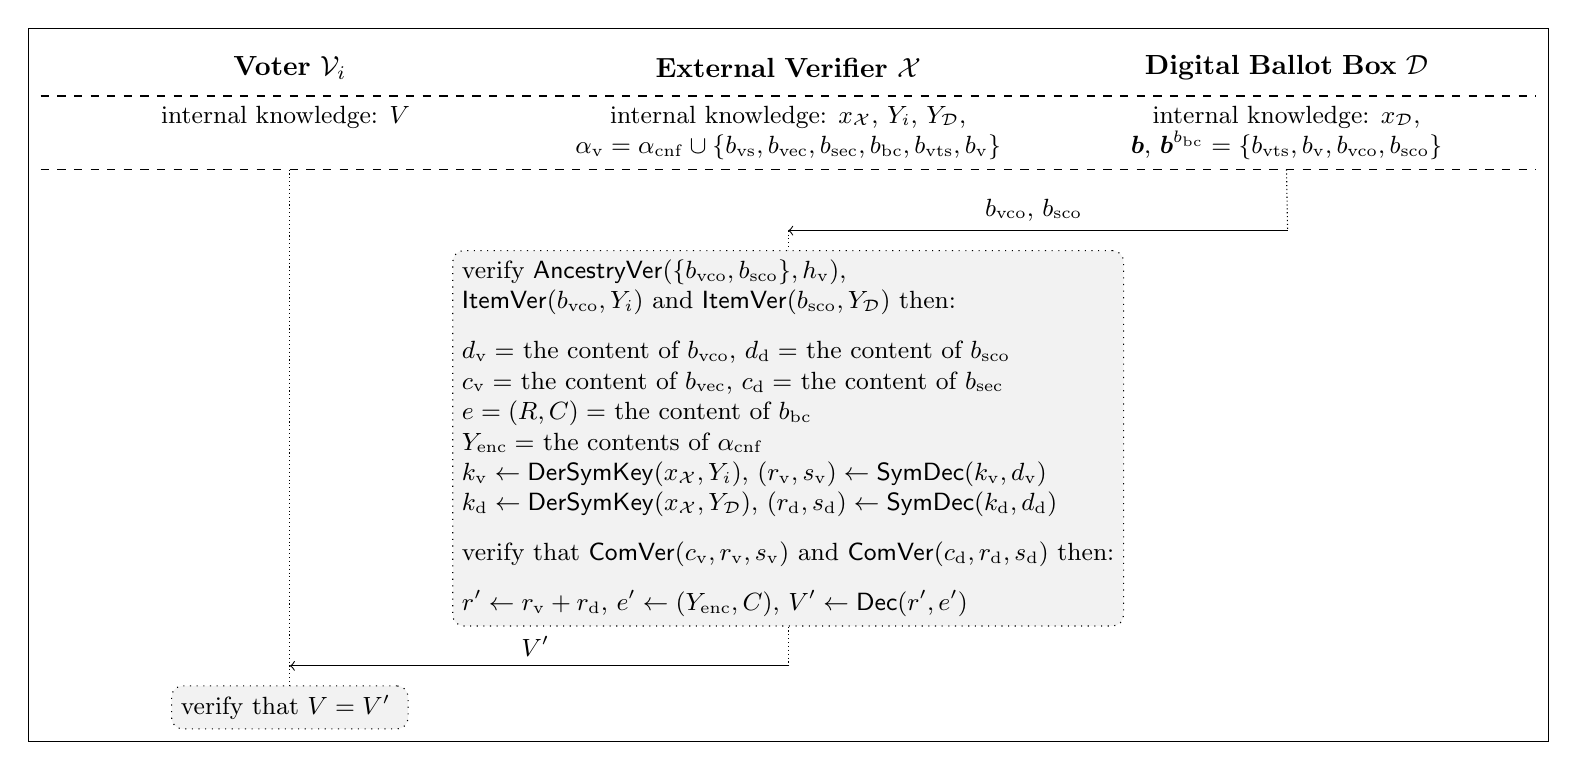
\begin{tikzpicture}[framed, node distance=0,
            % every node/.style={draw},
            ]{
        
        % Actors
        \node[title_3, above, anchor=north east] (v) {
            \textbf{Voter $\mathcal{V}_i$}};
        \node[title_3, right=of v] (ev) {
            \textbf{External Verifier $\mathcal{X}$}};
        \node[title_3, right=of ev] (dbb) {
            \textbf{Digital Ballot Box $\mathcal{D}$}};
        
        % internal knowledge
        \node[ik] at (v.south) (v_ik) {
            internal knowledge: $V$
            };
        \node[ik] at (ev.south) (ev_ik) {
            internal knowledge: $x_\mathcal{X}$, $Y_i$, $Y_\mathcal{D}$, \\
            $\alpha_\mathrm{v} = \alpha_\mathrm{cnf} \cup \{ b_\mathrm{vs}, b_\mathrm{vec}, b_\mathrm{sec}, b_\mathrm{bc}, b_\mathrm{vts}, b_\mathrm{v} \}$
            };
        \node[ik] at (dbb.south) (dbb_ik) {
            internal knowledge: $x_\mathcal{D}$, \\
            $\boldsymbol{b}$, $\boldsymbol{b}^{b_\mathrm{bc}} = \{ b_\mathrm{vts}, b_\mathrm{v}, b_\mathrm{vco}, b_\mathrm{sco} \}$
            };
        
        % All content
        \node[arrow, towards_left, spaced, between={ev.center}{dbb.center}] at (dbb_ik.south -| ev.center) (a_1) {
            $b_\mathrm{vco}$, $b_\mathrm{sco}$
            };
        \node[block, keep_middle, spaced] at (a_1.south -| ev.center) (ev_1) {
            verify $\mathsf{AncestryVer}(\{ b_\mathrm{vco}, b_\mathrm{sco} \}, h_\mathrm{v})$, \\
            $\mathsf{ItemVer} (b_\mathrm{vco},Y_i)$ and $\mathsf{ItemVer} (b_\mathrm{sco},Y_\mathcal{D})$ then: \\ [7pt]
            $d_\mathrm{v} = $ the content of $b_\mathrm{vco}$, $d_\mathrm{d} = $ the content of $b_\mathrm{sco}$ \\
            $c_\mathrm{v} = $ the content of $b_\mathrm{vec}$, $c_\mathrm{d} = $ the content of $b_\mathrm{sec}$ \\
            $e = (R, C) = $ the content of $b_\mathrm{bc}$ \\
            $Y_\mathrm{enc} = $ the contents of $\alpha_\mathrm{cnf}$ \\
            $k_\mathrm{v} \gets \mathsf{DerSymKey}(x_\mathcal{X}, Y_i)$, $(r_\mathrm{v}, s_\mathrm{v}) \gets \mathsf{SymDec}(k_\mathrm{v}, d_\mathrm{v})$ \\
            $k_\mathrm{d} \gets \mathsf{DerSymKey}(x_\mathcal{X}, Y_\mathcal{D})$, $(r_\mathrm{d}, s_\mathrm{d}) \gets \mathsf{SymDec}(k_\mathrm{d}, d_\mathrm{d})$ \\ [7pt]
            verify that $\mathsf{ComVer}(c_\mathrm{v}, r_\mathrm{v}, s_\mathrm{v})$
            and $\mathsf{ComVer}(c_\mathrm{d}, r_\mathrm{d}, s_\mathrm{d})$ then: \\ [7pt]
            $r' \gets r_\mathrm{v} + r_\mathrm{d}$, $e' \gets (Y_\mathrm{enc}, C)$, $V' \gets \mathsf{Dec}(r', e')$
            };
        \node[arrow, towards_left, between={v.center}{ev.center}] at (ev_1.south -| v.center) (a_2) {
            $V'$
            };
        \node[block, keep_middle, spaced] at (a_2.south -| v.center) (v_1) {
            verify that $V = V'$
            };
        
        % Arrows and lines
        \draw[dashed] (v.south west)--(dbb.south east);    
        \draw[dashed] (dbb_ik.south -| v.west)--(dbb_ik.south -| dbb.east);
        
        \draw[densely dotted] (dbb_ik.south -| v.center)--(v_1.north -| v.center);
        
        \draw[densely dotted] (a_1.south west)--(ev_1.north -| ev.center);
        \draw[densely dotted] (ev_1.south -| ev.center)--(a_2.south -| ev.center);
        
        \draw[densely dotted] (dbb_ik.south -| dbb.center)--(a_1.south east);
        }
    \end{tikzpicture}
    \caption{Unpacking the encrypted ballot protocol}
    \label{fig: unpacking the encrypted ballot protocol}
\end{figure}
\end{landscape}


\clearpage
\subsubsection{Vote confirmation receipt} \label{sec: vote confirmation receipt}
After encrypting a ballot, the voter $\mathcal{V}_i$ can choose whether to test or cast it. After choosing to cast the ballot, the voter receives a receipt from the digital ballot box that confirms that the ballot has been registered as cast on the public bulletin board. 

The voter has to follow the protocol from \cref{fig: ballot casting protocol} where the voting application interacts with the digital ballot box in $\mathtt{WriteOnBoard}(\mathcal{V}_i, m_\mathrm{cr}, c_\mathrm{cr}, p_\mathrm{cr})$ (protocol \ref{pro: write on board}) in order to append the cast request item $b_\mathrm{cr}$ on the board, where $m_\mathrm{cr} =$ "cast request", the content $c_\mathrm{cr}$ is empty and the parent $p_\mathrm{cr}$ is the address of the ballot cryptograms item $b_\mathrm{bc}$.

After publishing the cast request item on the bulletin board, the digital ballot box return to the voting app with the item $b_\mathrm{cr}$ and its receipt $\rho_\mathrm{cr}$. The voting app checks the item according to validations of protocol \ref{pro: write on board} and if valid, the voting application presents the receipt $\rho_\mathrm{cr}$ together with $\sigma_\mathrm{cr}$ and $h_\mathrm{cr}$ to the voter.

The voter stores the tuple as the vote confirmation receipt (i.e. proof of the ballot being cast on the bulletin board). The voter can use it at any time to check that the vote is registered on the bulletin board as described in \cref{sec: vote is registered as cast}.

Note that, if a voter $\mathcal{V}_i$ has a vote confirmation receipt $(\rho_\mathrm{cr}, \sigma_\mathrm{cr}, h_\mathrm{cr})$ that is valid (i.e. $\mathsf{SigVer}(Y_\mathcal{D}, \rho_\mathrm{cr}; \sigma_\mathrm{cr} || h_\mathrm{cr})$, where $Y_\mathcal{D}$ exists on the bulletin board $\boldsymbol{b}$) but does not correspond with the current state of the bulletin board (i.e. $h_\mathrm{cr}$ is not the address of any item of the bulletin board $\boldsymbol{b}$), that reveals that the integrity of the bulletin board has been broken and should be reported to the election officials.

\begin{figure}[ht]
    \centering
    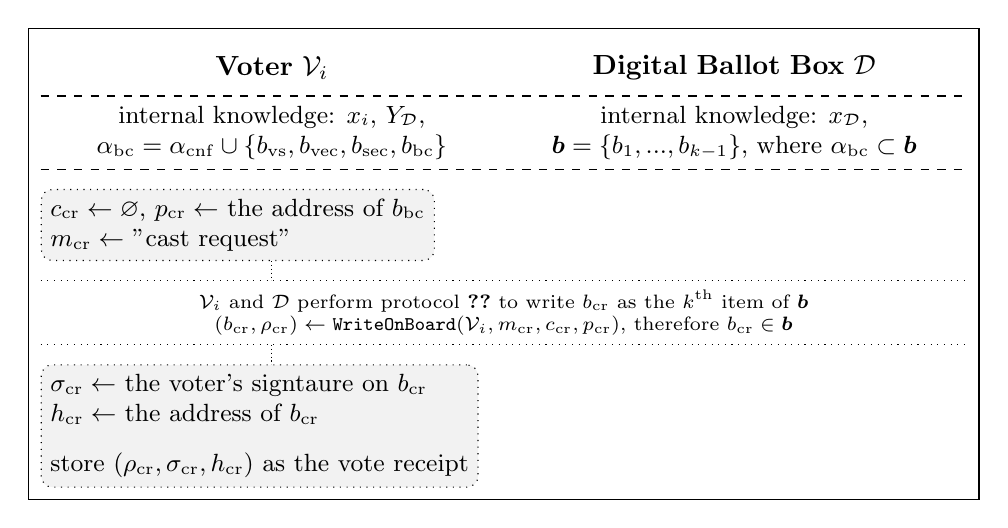
\begin{tikzpicture}[framed, node distance=0,
            % every node/.style={draw}
            ]{

        % Actors
        \node[title, above, anchor=north east] (v) {
            \textbf{Voter} $\mathcal{V}_i$};
        \node[title, right=of v] (dbb) {
            \textbf{Digital Ballot Box} $\mathcal{D}$};
        
        % internal knowledge
        \node[ik] at (v.south) (v_ik) {
            internal knowledge: $x_i$, $Y_\mathcal{D}$, \\
            $\alpha_\mathrm{bc} = \alpha_\mathrm{cnf} \cup \{ b_\mathrm{vs}, b_\mathrm{vec}, b_\mathrm{sec}, b_\mathrm{bc} \}$
            };
        \node[ik] at (dbb.south) (dbb_ik) {
            internal knowledge: $x_\mathcal{D}$, \\
            $\boldsymbol{b} = \{ b_1, ..., b_{k-1} \}$, where $\alpha_\mathrm{bc} \subset \boldsymbol{b}$
            };
        
        %All content
        \node[block, keep_left, spaced] at (dbb_ik.south -| v.west) (v_1) {
            $c_\mathrm{cr} \gets \varnothing$, $p_\mathrm{cr} \gets$ the address of $b_\mathrm{bc}$ \\
            $m_\mathrm{cr} \gets$ "cast request"
            };
        \node[banner, keep_left, spaced, between={v.west}{dbb.east}] at (v_1.south -| v.west) (b_1) {
            $\mathcal{V}_i$ and $\mathcal{D}$ perform protocol \ref{pro: write on board} to write $b_\mathrm{cr}$ as the $k^\mathrm{th}$ item of $\boldsymbol{b}$ \\
            $(b_\mathrm{cr}, \rho_\mathrm{cr}) \gets \mathtt{WriteOnBoard}(\mathcal{V}_i, m_\mathrm{cr}, c_\mathrm{cr}, p_\mathrm{cr})$, therefore $b_\mathrm{cr} \in \boldsymbol{b}$
            };
        \node[block, keep_left, spaced] at (b_1.south -| v.west) (v_2) {
            $\sigma_\mathrm{cr} \gets$ the voter's signtaure on $b_\mathrm{cr}$  \\
            $h_\mathrm{cr} \gets$ the address of $b_\mathrm{cr}$  \\ [7pt]
            store $(\rho_\mathrm{cr}, \sigma_\mathrm{cr}, h_\mathrm{cr})$ as the vote receipt
            };
        
        % Arrows and lines
        \draw[dashed] (v.south west)--(dbb.south east);    
        \draw[dashed] (dbb_ik.south -| v.west)--(dbb_ik.south -| dbb.east);

        \draw[dotted] (b_1.north west)--(b_1.north east);
        \draw[dotted] (b_1.south west)--(b_1.south east);
        
        \draw[densely dotted] (v_1.south -| v.center)--(b_1.north -| v.center);
        \draw[densely dotted] (b_1.south -| v.center)--(v_2.north -| v.center);
        }
    \end{tikzpicture}
    \caption{Ballot casting protocol}
    \label{fig: ballot casting protocol}
\end{figure}

\subsection{Post-election phase} \label{sec: post-election phase}
After the voting time has finished, the election proceeds to the last phase which will generate the result of the election. Now, the digital ballot box does not accept any new vote cryptograms anymore. The list of votes remains publicly available for voters to check that their vote cryptogram is included (using their confirmation receipt) and for auditors to check that the hash values of the list are consistent (the integrity of the board is persistent).

The process of computing a result consists of:
\begin{itemize}
    \item the election administrator requests a rezult to be computed by interacting with the digital ballot box in $\mathtt{WriteOnBoard}(\mathcal{E}, m_\mathrm{ei}, c_\mathrm{ei}, p_\mathrm{ei})$ (protocol \ref{pro: write on board}) to publish an extraction intent item $b_\mathrm{ei}$ on the bulletin board, according to the rules from \cref{app: bulletin board item types},
    \item the digital ballot box identifies all the valid ballots that are included in the tally, according to \cref{sec: cleansing procedure},
    \item a subset of all trustees $\boldsymbol{\mathcal{T}'} \subset \boldsymbol{\mathcal{T}}$ collaborate in the mixing process in order to anonymize the encrypted votes, as described in \cref{sec: mixing phase}, where $|\boldsymbol{\mathcal{T}'}| = n_\mathrm{d}$ and $t \leq n_\mathrm{d} \leq n_\mathrm{t}$ (recall from \cref{sec: threshold ceremony} that $t$ is threshold value for trustees and $\boldsymbol{\mathcal{T}} = \{ \mathcal{T}_1, ..., \mathcal{T}_{n_\mathrm{t}} \}$ is the set of all trustees),
    \item the same subset of trustees collaborate in the decryption process (\cref{sec: decryption phase}) of the anonymized votes,
    \item finally, the election administrator publishes the result in a verifiable manner as described in \cref{sec: result publication}.
\end{itemize}


\subsubsection{Cleansing procedure} \label{sec: cleansing procedure}
Triggered by the extraction intent item $b_\mathrm{ei}$ being published, the digital ballot box $\mathcal{D}$ bundles a list of cryptograms that represent only the valid votes from the ballot cryptograms items from the bulletin board. This is, essentially, the votes that will be decrypted and tallied as a result. It is considered a valid vote only the last ballot cryptograms item, followed by a cast request item for each voter. All other votes are considered overwritten and, therefore, discarded.

The list of cryptograms is called \textit{the initial mixed board} and it is defined as $\boldsymbol{e}_0 = \{ e_1, ..., e_{n_\mathrm{e}} \}$, with each $e_i \in \mathbb{E}$, where $\mathbb{E}$ is the set of all possible cryptograms and $n_\mathrm{e}$ is the total number of cryptograms. The list $\boldsymbol{e}_0$ is contained in an extraction data item $b_\mathrm{ed}$ published on the bulletin board by the digital ballot box $\mathcal{D}$ by running $\mathtt{WriteOnBoard}(\mathcal{D}, m_\mathrm{ed}, c_\mathrm{ed}, p_\mathrm{ed})$, where $m_\mathrm{ed} = $ "extraction data", the content $c_\mathrm{ed}$ is empty and the parent $p_\mathrm{ed}$ is the address of the extraction intent item $b_\mathrm{ei}$. The \textit{initial mixed board} $\boldsymbol{e}_0$ is used as the input to the mixing phase.

The cleansing procedure is publicly auditable as both the list of vote cryptograms and the \textit{initial mixed board} are publicly available.


\subsubsection{Mixing Phase} \label{sec: mixing phase}
During the mixing phase, the list of cryptograms will change its appearance several times, being shuffled in an indistinguishable way. Each trustee \( \mathcal{T}_i \in \boldsymbol{\mathcal{T}'} \) applies its mixing algorithm in sequential order (the output from $\mathcal{T}_{i-1}$ is the input to $\mathcal{T}_i$). The first trustee applies its algorithm on \textit{the initial mixed board} and the output of the last trustee is used as \textit{the final mixed board}. The election administrator facilitates the mixing phase and decides the order of trustees.

Formally, trustee $\mathcal{T}_i$ computes the mixed board of cryptograms by applying $\boldsymbol{e}_i \gets \mathsf{Shuffle}(Y_\mathrm{enc}, \boldsymbol{e}_{i-1}, \boldsymbol{r}_i, \psi_i)$ (\cref{alg: shuffle}), where $Y_\mathrm{enc}$ is the encryption key, $\boldsymbol{r}_i \in \mathbb{Z}_q^{n_\mathrm{e}}$ and $\psi_i$ is a permutation of $n_\mathrm{e}$ elements. Next, as described in \cref{app: groth's argument of shuffle}, trustee $\mathcal{T}_i$ computes a proof of correct mixing $(PM_i, AS_i) \gets \mathsf{ProveMix}(\psi_i, Y_\mathrm{enc}, \boldsymbol{r}_i, \boldsymbol{e}_{i-1}, \boldsymbol{e}_i)$ (\cref{alg: prove mix}). Then, trustee $\mathcal{T}_i$ submits to the election administrator the mixed board $\boldsymbol{e}_i$ and the mixing proof $(PM_i, AS_i)$.

For a mixing step to be accepted, the validity of the mixing proof has to be checked by running $\mathsf{VerMix}(PM_i, AS_i, Y_\mathrm{enc}, \boldsymbol{e}_{i-1}, \boldsymbol{e}_i)$ (\cref{alg: ver mix}). In case a proof fails, either that trustee recomputes the mixing step, or it is removed and the process continues without that trustee.

Obviously, each trustee $\mathcal{T}_i$ knows the shuffling coefficients ($\boldsymbol{r}_i$ and $\psi_i$) of its own mixing algorithm and it is able to link the votes on the previous mixed board $\boldsymbol{e}_{i-1}$ with the ones on the mixing board at $i^\mathrm{th}$ step $\boldsymbol{e}_i$. However, $\mathcal{T}_i$ does not know the shuffling coefficients of the other trustees so it cannot create a full link between the votes on the \textit{final mixed board} and the ones on the \textit{initial mixed board}, unless all trustees are corrupt and collude against the election.

Assuming there is at least one honest trustee that will not reveal its shuffling coefficients, then the \textit{final mixed board} of cryptograms represents the anonymized version of the \textit{initial mixed board} of cryptograms. The \textit{final mixed board} of cryptograms is used in the decryption phase to compute the election results.


\subsubsection{Decryption Phase} \label{sec: decryption phase}
Because the link between a vote cryptogram and its voter has been broken during the mixing phase, it is safe now to decrypt all the cryptograms from the \textit{final mixed board} as it does not violate the secrecy of the election. Furthermore, decrypting this list of cryptograms would lead to accurate and correct results as it contains the exact same votes as the initial list of votes, fact proven by the mixing proofs. In this section, the \textit{final mixed board} is reffered to as $\boldsymbol{e}$.

During the decryption phase, trustees have to collaborate again to perform the threshold decryption protocol as presented in \cref{fig: threshold decryption}. Each trustee \( \mathcal{T}_i \in \boldsymbol{\mathcal{T}'} \) gets the \textit{final mixed board} of cryptograms $\boldsymbol{e} = \{ e_1, ..., e_{n_\mathrm{e}} \}$ then computes partial decryptions of each cryptogram together with a proof of correct decryption by applying $(\boldsymbol{S}_i, PK_i) \gets \mathsf{PartiallyDecryptAndProve}(\boldsymbol{e}, sx_i)$ (\cref{alg: partially decrypt and prove}). Recall that, trustee $\mathcal{T}_i$ is in possession of its share of the decryption key $sx_i$ as it has been computed during the threshold ceremony (\cref{sec: threshold ceremony}).

Then, trustee $\mathcal{T}_i$ submits the partial decryption $\boldsymbol{S}_i$ and the proof $PK_i$ to the election administrator service, which in \cref{fig: threshold decryption} is reffered to as \textit{the server}. The election administrator accepts the partial decryption if the proof validates according to $\mathsf{PartialDecryptionVer}(\boldsymbol{e}, \boldsymbol{S}_i, PK_i, sY_i)$ (\cref{alg: partial decryption ver}), where $sY_i$ is the public share of the trustee $\mathcal{T}_i$ and it is computable as in \cref{app: elgamal threshold cryptosystem}.

Upon receiving partial decryptions $\boldsymbol{S}_1, ..., \boldsymbol{S}_{n_\mathrm{d}}$ from all trustees in $\boldsymbol{\mathcal{T}'}$, the election administrator follows the protocol from \cref{fig: threshold decryption} and aggregates all partial decryptions for each cryptogram in $\boldsymbol{e}$ to finalize the decryption and extract the votes $\boldsymbol{V} = \{ V_1, ..., V_{n_\mathrm{e}} \} \gets \mathsf{FinalizeDecryption} (\boldsymbol{e}, \boldsymbol{S}_1, ..., \boldsymbol{S}_{n_\mathrm{d}})$ (\cref{alg: finalize decryption}). $\boldsymbol{V}$ represents the \textit{raw result} of the election, i.e. the full list of votes as elliptic curve points.

\begin{algorithm}[ht]
    \DontPrintSemicolon
    \caption{$\mathsf{PartiallyDecryptAndProve}(\boldsymbol{e}, sx)$}
    \KwData{The list of cryptograms $\boldsymbol{e} = \{e_1, ..., e_n\} \in \mathbb{E}^n$, with $e_i = (R_i, C_i)$}
    \myinput{The share of decryption key $sx \in \mathbb{Z}_q$}
    
    \For{$i \gets 1$ \KwTo $n$ \KwBy $1$}{
        $S_i \gets [sx]R_i$
        }
    $\boldsymbol{S} \gets \{S_1, ..., S_n\}$ \;
    $\boldsymbol{R} \gets \{R_1, ..., R_n\}$ \;
    $PK \gets \mathsf{DLProve}(sx, \boldsymbol{R})$ \tcp*{\cref{alg: dl prove}}
    
    \Return{$(\boldsymbol{S}, PK)$} \tcp*{$\boldsymbol{S} \in \mathbb{P}^n$, $PK \in \mathbb{P} \times \mathbb{Z}_q \times \mathbb{Z}_q$}
    
    \label{alg: partially decrypt and prove}
\end{algorithm}

\begin{algorithm}[ht]
    \DontPrintSemicolon
    \caption{$\mathsf{PartialDecryptionVer}(\boldsymbol{e}, \boldsymbol{S}, PK, sY)$}
    \KwData{The list of cryptograms $\boldsymbol{e} = \{e_1, ..., e_n\} \in \mathbb{E}^n$, with $e_i = (R_i, C_i)$}
    \myinput{The list of partial decryptions $S = \{ S_1, ..., S_n \} \in \mathbb{P}^n$}
    \myinput{The proof of correct decryption $PK \in \mathbb{P} \times \mathbb{Z}_q \times \mathbb{Z}_q$}
    \myinput{The public share of decryption key $sY \in \mathbb{P}$}
    
    $\boldsymbol{R}' \gets \{G, R_1, ..., R_n\}$ \;
    $\boldsymbol{S}' \gets \{sY, S_1, ..., S_n\}$ \;
    $b \gets \mathsf{DLVer}(PK, \boldsymbol{R}', \boldsymbol{S}')$ \tcp*{\cref{alg: dl ver}}
    
    \Return{$b$} \tcp*{$b \in \mathbb{B}$}
    
    \label{alg: partial decryption ver}
\end{algorithm}

\begin{algorithm}[ht]
\DontPrintSemicolon
    \caption{$\mathsf{FinalizeDecryption} (\boldsymbol{e}, \boldsymbol{S}_1, ..., \boldsymbol{S}_{n_\mathrm{d}})$}
    \KwData{The list of cryptograms $\boldsymbol{e} = \{ e_1, ..., e_n \} \in \mathbb{E}^n$, with $e_j = (R_j, C_j)$}
    \myinput{The partial decryptions $\boldsymbol{S}_i = \{ S_{i, 1}, ..., S_{i, n} \} \in \mathbb{P}^n$, where $\mathcal{T}_i \in \boldsymbol{\mathcal{T'}}$}
    
    \For{$j \gets 1$ \KwTo $n$ \KwBy $1$}{
        $V_j \gets C_j - \sum_{i \in \boldsymbol{\mathcal{T}'}} [\lambda(i)]S_{i,j}$ \tcp*{$\lambda(i)$ computed as in figure \ref{fig: threshold decryption}}
        }
    $\boldsymbol{V} \gets \{ V_1, ..., V_n \}$ \;
    
    \Return{$\boldsymbol{V}$} \tcp*{$\boldsymbol{V} \in \mathbb{P}^n$}
    
    \label{alg: finalize decryption}
\end{algorithm}


\subsubsection{Result Publication} \label{sec: result publication}
The \textit{results module} is responsible for interpreting the \textit{raw result} and present the result of the election in a more readable way. The interpretation of the result is dependant on the election type (simple election, multiple election, STV, etc.).

For simplicity, we will consider the simple election case, where voters had to choose one option from a predefined set of candidates, i.e. a vote is a plain text that represents a candidate name.

First, all votes $V_i \in \boldsymbol{V}$ have to be decoded into bytes $\boldsymbol{b}_i \gets \mathsf{Point2Bytes}(V_i)$ (\cref{alg: point to bytes}), then interpreted as text and finally mapped to one of the candidate names. If any of these steps fail, then the vote $V_i$ is considered invalid. Tallying the votes that each candidate received is considered trivial and out of scope for this document.

Finally, all data that has been computed in the result ceremony (both mixing and decryption phases) is collected by the election administrator $\mathcal{E}$, and published on the bulletin board as the extraction confirmation item $b_\mathrm{ec}$ by performing $\mathtt{WriteOnBoard}(\mathcal{E}, m_\mathrm{ec}, c_\mathrm{ec}, p_\mathrm{ec})$ (protocol \ref{pro: write on board}), where $m_\mathrm{ec} = $ "extraction confirmation", the parent $p_\mathrm{ec}$ is the address of the extraction data item $b_\mathrm{ed}$  and the content $c_\mathrm{ec}$ consists of:
\begin{itemize}
    \item a set of the following data from each trustee that participated in the result ceremony $\mathcal{T}_i \in \boldsymbol{\mathcal{T}'}$:
    \begin{itemize}
        \item the mixed boards of cryptograms $\boldsymbol{e}_i$
        \item the mixing proofs $(PM_i, AS_i)$
        \item the partial decryptions $\boldsymbol{S}_i$
        \item the proofs of correct decryption $PK_i$
    \end{itemize}
    \item the list of decrypted votes $\boldsymbol{V}$
    \item the summarized (tallied) election result
\end{itemize}

\subsection{Election properties} \label{sec: election properties}
\paragraph{Eligibility}
During the \textit{pre-election phase} (\cref{sec: pre-election phase}), the \textit{election administrators} define the list of eligible voters \( \boldsymbol{\mathcal{V}} = \{\mathcal{V}_1, ..., \mathcal{V}_{n_\mathrm{v}}\} \), where $n_\mathrm{v}$ is the total number of voters, and the list of printing authorities \( \boldsymbol{\mathcal{P}} = \{\mathcal{P}_1, ..., \mathcal{P}_{n_\mathrm{p}}\} \), where $n_\mathrm{p}$ is the total number of printing authorities.

During the \textit{voter credential distribution process} (\cref{sec: voter credential distribution process}), all \textit{printing authorities} assign a distinct public signature verification key $Y_i$ to each voter $\mathcal{V}_i$. At the same time, each \textit{printing authority} \( \mathcal{P}_j \in \boldsymbol{\mathcal{P}} \) distributes to each voter their voting credentials $x_{i,j}$, with \( i \in \{ 1, ..., n_\mathrm{v} \} \) and \( j \in \{ 1, ..., n_\mathrm{p} \} \) such that \( [\sum_{j=1}^{n_\mathrm{p}} x_{i,j}]G = Y_i \). After receiving all his election credentials $x_{i,j}$, voter $\mathcal{V}_i$ can compute his private signing key \( x_i = \sum_{j=1}^{n_\mathrm{p}} x_{i,j} \).

When submitting a vote, the voter $\mathcal{V}_i$ digitally signs the vote submission with his private signing key $x_i$ and the election system accepts the vote submission only if the digital signature matches the voter's public signature verification key $Y_i$. By following this process, we make sure that the vote submission was generated by somebody in possession of $x_i$, which could only be the voter.

One can notice that the printing authority $\mathcal{P}_j$ knows a part of the signing key of voter $\mathcal{V}_i$ but not enough. Therefore, we argue that Assembly Voting X has the \textit{eligibility property} on the assumption that there exist multiple printing authorities that do not communicate with each other during the election process.

\paragraph{No revealing of partial results // fairness}
By following the election protocol, it is guaranteed that:
\begin{itemize}
    \item the secrecy of the vote is preserved. No votes from the bulletin board are decrypted, therefore no connection between a vote and a voter can be made.
    \item no partial results are computed during the election process. A result is calculated only once, after the election phase has finished. This prevents influencing of the subsequent voters throughout the election period.
\end{itemize}

All votes, that are posted on the bulletin board, are encrypted using the ElGamal cryptosystem based on elliptic curve cryptography (more details in \cref{app: mathematics} and \cref{app: elgamal cryptosystem}). Moreover, using a \textit{t out of n} threshold encryption scheme (\cref{sec: threshold ceremony}), we enforce that there is no single entity that can perform the decryption of any data from the public bulletin board, but instead, it is needed a group of minimum $t$ trustees to collaborate.

Therefore, we claim that Assembly Voting X has the \textit{confidentiality property} on the assumption that at least $t$ trustees are honest, with \( t > n / 2 \) and \( n > 2 \).

One can argue that, because the bulletin board data is public, somebody could save all the data for long enough until the elliptic curve cryptosystem will be broken, and so will be able to decrypt all the data contrarily to our protocol. This fact demonstrates that our system does not comply to the \textit{everlasting confidentiality property}. We take note of this fact and we accept it.

\paragraph{Anonymity}
This property is reached by implementing a mixnet of nodes (trustees) that sequentially shuffle the list of vote cryptograms in an indistinguishable way, before they get decrypted (\cref{sec: mixing phase}).

Obviously, each trutsee knows the way it shuffled the list of cryptograms but it does not know how it was shuffled by the other trustees. Thus, it is important that trustees do not communicate with each other.

We claim that Assembly Voting X is an \textit{anonymous voting system} on the assumption that there is a set of multiple trustess out of which at least one is honest.

\paragraph{Integrity}
The integrity of the election is preserved in our system by publishing all events (vote submissions or system events) on the bulletin board. Moreover, the bulletin board has a \textit{blockchain-like} structure that guarantees that the history of the bulletin board never changes. Also, the voters act like miners of the blockchain whenever they submit a new vote cryptogram, by signing on the history of the blockchain.

Every time a new vote submission is appended on the bulletin board, the voter receives a vote receipt $\rho_i$ that contains a pointer to the item on the bulletin board, called \textit{the board hash value} $h_{\mathrm{b}, i}$. This value is computed based on the previous \textit{board hash value} $h_{\mathrm{b}, i-1}$, which is computed based on the one before, and so on, until it reaches the \textit{genesis hash}, which is 0. This means that every time a voter checks his voter receipt, the entire bulletin board history is validated.

We claim that Assembly Voting X achieves the \textit{integrity property} through the bulletin board construction.

\paragraph{Verifiability}
There are two levels of verifiability that can be performed by different actors. Some steps are individually verifiable (i.e. only the voter that is currently performing this step can verify that the process is happening correctly), such as:
\begin{itemize}
    \item verify that the vote is cast as intended
    \item verify that the vote is registered as cast
\end{itemize}
The rest of the steps from the election protocol are publicly verifiable:
\begin{itemize}
    \item the threshold ceremony
    \item the bulletin board history
    \item the integrity and eligibility of each vote submission
    \item the integrity of each system event
    \item the correctness of the cleansing procedure, mixing phase and decryption phase (verification that votes are counted as registered)
\end{itemize}

We claim that Assembly Voting X is a \textit{verifiable election system}.

% \subsection{Accountability}
\paragraph{Receipt-freeness}
During the \textit{vote cryptogram generation process} (described in \cref{sec: vote cryptogram generation process}), the voter receives from the \textit{Digital Ballot Box} $\mathcal{D}$ an empty cryptogram $e_0$ that he uses to generate his final vote cryptogram $e$ in order to encrypt his vote $M$. At the end of the process, the vote cryptogram $e$ would be equal to \( \mathsf{Enc} (Y_\mathrm{enc}, M, r_0 + r_1) \), where $r_0$ is known by the \textit{Digital Ballot Box} $\mathcal{D}$ and $r_1$ is known by the voter.

% The voter is convinced that $e_0$ is an empty cryptogram because of a interactive proof $PK_0$ generated between the voter and the \textit{Digital Ballot Box} $\mathcal{D}$.

% The empty cryptogram $e_0$ and the proof $PK_0$ are relevant only for the communication amongst the voter and the \textit{Digital Ballot Box} $\mathcal{D}$, to make sure that none of them has the entire randomness value $r_0 + r_1$ that is used to generate the cryptogram $e$. Therefore, $e_0$ and $PK_0$ are not included on the bulletin board, thus not publicly available.

After the vote cryptogram $e$ has been accepted on the bulletin board, the voter is not able to produce valid cryptographic evidence that $e$ is an encryption of $M$ referencing only the data that is publicly available, as he is not in possession of value $r_0$. More details are described in \cref{app: proving the content of a cryptogram}.

Therefore, we claim that Assembly Voting X is a \textit{receipt-free} voting protocol.

\clearpage
\section{Auditing} \label{sec: auditing}
This section describes the entire auditing process of an election. It describes all the verification mechanisms, who conducts them, and what cryptographic algorithms they involve. These verification mechanisms can be split into three categories:
\begin{itemize}
    \item voter-specific verification mechanisms that can be performed individually by voters and target their specific vote (\cref{sec: voter-specific verifications}),
    \item internal auditing processes performed by election officials that target the behavior of the election system (\cref{sec: administration auditing process}),
    \item publicly available audit processes that verify all data on the public bulletin board (\cref{sec: public auditing process}).
\end{itemize}

\subsection{Voter-specific verifications} \label{sec: voter-specific verifications}
During the voting process, voters can verify two aspects of their vote: that it is cast as intended and registered as cast. These verification steps help voters gain confidence that the election system behaves correctly, at least at processing their vote.


\subsubsection{Vote is cast as intended}
At the end of the vote cryptogram generation process (\cref{sec: vote cryptogram generation process}), the voter is presented with cryptogram $e = (R, C)$, which is the encryption of vote $V$ with the encryption key $Y_\mathrm{enc}$ and randomizer $r = r_\mathrm{v} + r_\mathrm{d}$, where $r_\mathrm{v}$ is known by the voting application and $r_\mathrm{d}$ is known only by the digital ballot box. Hence, it is the voting application and the digital ballot box that collectively perform the encryption of the voter's vote.

Because the vote is encrypted, the voter cannot tell whether cryptogram $e$ actually represents an encryption of vote $V$ or not. Therefore, to get convinced that the voting application and the digital ballot box behaved correctly during the vote cryptogram generation process, the voter can perform a challenge of the vote cryptogram, as presented in \cref{sec: challenging a vote cryptogram} to verify the activity of the voting application and digital ballot box.

If the voter chooses to challenge the cryptogram, a second device is used to perform all the cryptographic validations on behalf of the voter. Both randomizers $r_\mathrm{v}$ and $r_\mathrm{d}$ are sent securely from the voting application and the digital ballot box, respectively, to the external verifier application that runs on the secondary device. The verification application uses them to unpack the encrypted ballot and present the vote choices to the voter. The fully detailed process is shown in \cref{sec: challenging a vote cryptogram}.

If the vote corresponds to the voter's intended choices, then the voter gains confidence that the voting application behaved correctly.

If the vote does not correspond to the voter's intention, the auditing process provides evidence that the encrypted ballot has not been cast as intended. Note that, in this case, there is no distinction between the election system maliciously changing the voter's vote behind the scenes or the voter accidentally mischoosing the vote options.

After the voter has successfully audited the vote, it gets invalidated because the randomizer value $r_\mathrm{v} + r_\mathrm{d}$ has been exposed. Now, the voter has to regenerate a vote cryptogram (as presented in \cref{sec: vote cryptogram generation process}) and choose again whether to challenge or submit. Voters should challenge again until they have enough confidence in the election system to cast their vote as intended.

 
\subsubsection{Vote is registered as cast} \label{sec: vote is registered as cast}
When the voter submits and casts an encrypted ballot (by submitting a cast request item as described in \cref{sec: vote confirmation receipt}), a receipt $\rho$ is returned as a response from the digital ballot box. The receipt contains a digital signature of the digital ballot box, which certifies that the voter's ballot has been registered on the public bulletin board. The receipt can be validated by checking $\mathsf{SigVer} (Y_\mathcal{D}, \rho; \sigma || h)$ (\cref{alg: sig ver}), where $Y_\mathcal{D}$ is the public key of the digital ballot box, $\sigma$ is the voter's signature on the cast request item, and $h$ is the address of the item on the bulletin board.

Anytime after casting a ballot, the voter can check the receipt against the bulletin board, which should find the appropriate ballot submission. Thus, the voter gains confidence that the vote is registered as cast.

If a voter has a valid receipt (i.e., which validates $\mathsf{SigVer} (Y_\mathcal{D}, \rho; \sigma || h)$) that does not correspond to any item from the public bulletin board, then the receipt $\rho$ represents evidence that the integrity of the bulletin board has been compromised. The argument is that a previously accepted item has been removed or tampered with on the bulletin board.

\subsection{Administration auditing process} \label{sec: administration auditing process}
This process is only relevant if the voter authentication mode \textbf{identity-based} described in \cref{sec: identity-based mode} is used. This auditing is private since the identification token contains the voter's identity information such an email address which is sensitive information that cannot be publicly accessible and must be audited privately within the system's borders.

% Private auditing process are only accessible to the internal verification of AVX. This type of verification is only used during the voter authentication mode \textbf{identity-based} described in \cref{sec: identity-based mode}. This process is used when the identification and authentication of a user has to be audited during post-election. The private auditing process is used when auditing each users' confirmation token, authentication token, and public key.

\subsubsection{Eligibility verifiability}
During the post-election the entire bulletin board is audited. The auditor needs to be provided with the list of eligible voters $\boldsymbol{\mathcal{V}}$ from the \textit{Election Administrator} $\mathcal{E}$. The auditor also need to be provided with all identity tokens from the \textit{Identity Provider} $\mathcal{I}$. All authentication tokens and public keys are provided through the \textit{Digital Ballot Box} $\mathcal{D}$. The Auditor is also required to be provided the list that links the identity and authentication tokens with a voter that the \textit{Voter Authorization Service} $\mathcal{A}$ stores. 

The private auditor validates the signature of the identity token, authentication token, and public key by \( \mathbf{VerifySignature}_{Y_i} (\sigma, h_\mathrm{v}) \) (\cref{alg: sig ver}). The auditor checks for each authentication token that their individual link to a identity token matches the link the \textit{Voter Authorization Service} $\mathcal{A}$ has. It is also checked that the link in the public key token of the \textit{Voter} $\mathcal{V}$ is linked to the same identity token. The private auditor also verifies that the identity of \textit{Voter} $\mathcal{V}_i$ that is in the identity token is also on the list of eligible voters $\mathcal{V}_i \in \boldsymbol{\mathcal{V}}$. 

\subsection{Public auditing process} \label{sec: public auditing process}
Public auditing processes are accessible to anybody. They are used to validate that the entire election is run correctly. This audit is typically run at the end of the election period by certified auditors that will validate or invalidate an election result. Nevertheless, it could be run both during the election phase or when the election has finished by any public person with access to the public bulletin board and suitable verification algorithms.

As part of the public auditing, the following verification steps are included:
\begin{itemize}
    \item During the election phase and after the election has finished, anybody can verify the integrity of the data published on the bulletin board, as explained in \cref{sec: integrity of the bulletin board}.
    \item After a result has been initiated (i.e., an extraction data item has been published as in \cref{sec: cleansing procedure}), anybody can verify that the cleansing procedure has been performed correctly, as explained in \cref{sec: verification of the cleansing procedure}.
    \item After a result has been computed and published, any public auditor can check the correctness of the result by verifying both the mixing process (see \cref{sec: verification of mixing procedure}) and the decryption process (see \cref{sec: verification of decryption}).
\end{itemize}

By having the election result auditable, the election protocol achieves one of the end-to-end verifiability properties, i.e., verification that all votes have been counted as registered.


\subsubsection{Integrity of the bulletin board} \label{sec: integrity of the bulletin board}
This verification step checks that only qualified actors have published items on the bulletin board. It also checks that no items have been removed or tampered with once posted on the bulletin board. This is achieved by checking the integrity of the hash structure of the bulletin board (referred to as the \textit{history} property of the bulletin board in \cref{sec: public bulletin board}) and by checking the validity of the digital signatures of each item.

Formally, given a complete bulletin board or a portion of it, in the form of a list of items $\boldsymbol{b} = \{ b_1, ..., b_n \}$, any public auditor can check the integrity of the list by running $\mathsf{HistoryVer} (\boldsymbol{b}, h'_1)$ (\cref{alg: history ver}), where $h'_1$ is the address of the previous item in the history. When $\boldsymbol{b}$ is a complete bulletin board (i.e., $b_1$ is a genesis item), then $h'_1$ must be equal to $\varnothing$, as the genesis item has no previous address.

Additionally, the auditor checks the correctness of the chosen parameters of each item $b_i \in \boldsymbol{b}$ (i.e., that it has a properly structured content $c_i$ and that it references a proper parent $p_i$ both according to the rules specified in \cref{app: bulletin board item types}). Then the auditor validates the integrity of each item by $\mathsf{ItemVer} (b_i, Y_{\mathcal{W}_i})$, where $Y_{\mathcal{W}_i}$ is the public key of the writer of the $i^\mathrm{th}$ item. Note that, as described in \cref{app: bulletin board item types}, depending on the type of item, one of the following actors can be the writer of an item: the digital ballot box $\mathcal{D}$, the election administrator $\mathcal{E}$, the voter authorizer $\mathcal{A}$ or a specific voter $\mathcal{V}$. The public key of any of these actors must be retrieved from the content of the bulletin board itself, such as:
\begin{itemize}
    \item the public keys of the election administrator $Y_\mathcal{E}$ and of the digital ballot box $Y_\mathcal{D}$ are listed in the genesis item,
    \item the public key of the voter authorizer $Y_\mathcal{A}$ is listed in an actor configuration item that defines the voter authorizer role,
    \item each public key $Y_j$ of the $j^\mathrm{th}$ voter is introduced by a voter session item.
\end{itemize}

If any verification steps mentioned above fail, then $\boldsymbol{b}$ does not represent a valid bulletin board trace.


\subsubsection{Verification of the cleansing procedure} \label{sec: verification of the cleansing procedure}
Given a bulletin board trace $\boldsymbol{b}$, with an extraction data item included in $\boldsymbol{b}$, any public auditor can verify the correctness of the list of cryptograms $\vec{\vec{e}}_0$ present in the extraction data item. Recall from \cref{sec: cleansing procedure} that $\vec{\vec{e}}_0$ lists all votes that will make up the election result.

The auditor reruns the cleansing procedure on the bulletin board $\boldsymbol{b}$, applying all the filtering rules specified in \cref{sec: cleansing procedure} to recompute the \textit{initial mixed board} $\vec{\vec{e}}_0^{\, \prime}$. If $\vec{\vec{e}}_0^{\, \prime}$ is identical with $\vec{\vec{e}}_0$, then the cleansing procedure has been performed correctly.


\subsubsection{Verification of mixing procedure} \label{sec: verification of mixing procedure}
After a result has been published via an extraction confirmation item (as described in \cref{sec: result publication}), any public auditor can verify the mixing procedure of each trustee that participated in the mixing phase. This checks that no votes have been tampered with during mixing. The data that an auditor needs to collect comes from the following sources:
\begin{itemize}
    \item the initial mixed board $\vec{\vec{e}}_0$ is listed in the extraction data item,
    \item the encryption keys $Y_\mathrm{enc}$ and the list of trustees $\boldsymbol{\mathcal{T}} = \{ \mathcal{T}_1, ..., \mathcal{T}_{n_\mathrm{t}} \}$ are listed in the threshold configuration item, where $n_\mathrm{t}$ is the amount of trustees,
    \item the subset of trustees that participated in the mixing and decryption phases $\tau \subset \{ 1, ..., n_\mathrm{t} \}$, together with all the intermediate mixed boards that they produced $\vec{\vec{e}}_i$, with $i \in \tau$, and their respective proofs of correct mixing $(PM_i, AS_i)$ are included in the extraction confirmation item.
\end{itemize}

The auditor validates each intermediate mixed board by running \cref{alg: mix ver} $\mathsf{MixVer} (PM_i, AS_i, Y_\mathrm{enc}, \vec{\vec{e}}_{i-1}, \vec{\vec{e}}_i)$, for each $i \in \tau$. If any validations fail, the published result is not trustworthy.


\subsubsection{Verification of the decryption} \label{sec: verification of decryption}
After a result has been published via an extraction confirmation item (as described in \cref{sec: result publication}), any public auditor can verify the decryption procedure by checking all the partial decryptions of each trustee that participated in the decryption phase. The data that an auditor needs to collect comes from the following sources:
\begin{itemize}
    \item the list of all trustees $\boldsymbol{\mathcal{T}} = \{ \mathcal{T}_1, ..., \mathcal{T}_{n_\mathrm{t}} \}$, together with their public keys $\{ Y_{\mathcal{T}_1}, ..., Y_{\mathcal{T}_{n_\mathrm{t}}} \}$ and public polynomial coefficients $\{ P_{\mathcal{T}_1, 1}, ..., P_{\mathcal{T}_{n_\mathrm{t}}, t-1} \}$, are listed in the threshold configuration item, where $t$ is the threshold value set during the threshold ceremony (see \cref{sec: threshold ceremony}), and $n_\mathrm{t}$ is the total number of trustees,
    \item the final mixed board $\vec{\vec{e}}$ is listed in the extraction confirmation item,
    \item the subset of trustees that participated in the mixing and decryption phases $\tau \subset \{ 1, ..., n_\mathrm{t} \}$, together with all their partial decryption $\vec{\vec{S}}_i$, with $i \in \tau$, and their respective proofs of correct decryption $PK_i$ are also included in the extraction confirmation item.
\end{itemize}

The auditor validates the proof of each partial decryption by running \cref{alg: partial decryption ver} $\mathsf{PartialDecryptionVer} (\vec{\vec{e}}, \vec{\vec{S}}_i, PK_i, sY_i)$, for each $i \in \tau$, where $sY_i$ is the public share of the trustee $\mathcal{T}_i$ computed as in \cref{app: threshold cryptosystem}.

If all partial decryptions are valid, the auditor aggregates them together to recompute the raw result $\vec{\vec{V}} \gets \mathsf{FinalizeDecryption} (\vec{\vec{e}}, \{ \vec{\vec{S}}_i | i \in \tau \})$ (\cref{alg: finalize decryption}). The list of decrypted votes $\vec{\vec{V}}$ should be identical to the published result. If any validation step fails, the result is considered untrustworthy.

Counting the votes and sorting the candidates based on their vote count is considered trivial and out of scope.

\clearpage
\section{Threat model} \label{sec: threat model}

% \subsection{Trust, actors and channels} 
This paper has dealt with trust-independent processes. These processes are characterized by the ability to mathematically prove the entirety of operations.

An example of a trust-independent process is an actor casting a ballot encrypted by the election public key and signed by a private key. Arriving in the Digital Ballot Box, it can be proven that this ballot was indeed encrypted and signed with the aforementioned keys.

Trust-independent processes must be audited to ensure integrity of the election. The result of such an audit will always be binary - either the process was successful or not. It is not conceivable that a cryptographically backed process executes in a partly successful way. Furthermore the binary characteristics of a trust-independent process signals that there are no exploits that can be mitigated. It either works by its inherent mathematical properties or it doesn’t.

Trust-independent processes are often extremely narrowly defined to align with the mathematics. Consider an attempt to describe the same process as the above in layman’s terms: “The voter uses an internet connected mobile phone to cast the ballot safely to the Digital Ballot Box.”. The trust-independent process of encryption and signing is a part of this process description, but it is also clear that many trust-dependent assumptions were introduced, for example the assumption that the voter is an eligible voter, that the mobile phone is not compromised and that the communication channel (network) was available. All such trust-dependent assumptions must be dealt with in a threat model.

It is important to stress that even if we say that a process supported by cryptography is trust-independent, we ultimately place trust in the deployed scientifically validated cryptographic methods, both at the level of mathematics and the actual implementation in code.

The threat model will concentrate on the trust-dependent process. By trust-dependance we mean a quality/property that is not backed by cryptography and cannot be mathematically proven.

Trust-dependent processes can be a lot of things. In essence they consist of actors which can be a person (like an IT-administrator, an Election Officer, etc.) or a system (like the Digital Ballot Box, The Voter Authorizer, etc.). Also actors will often communicate with each other through some sort of channel (i.e. HTTPS).

Examples of trust-dependent processes are an IT-administrator (actor) who we trust will configure the system in a prescribed and honest way, or a display or keyboard (actor) which we trust will transfer (channel) the intended information to/from a user or voter.

Trust-dependent processes can (and should extensively) be audited, but the bottom line is that the room for exploits will always remain more or less open no matter what level of mitigation measures that are deployed.

% \subsection{Trust-dependent assumptions} 
The threats against a system can be derived from the built-in trust-dependent assumptions. The following will list the processes in various phases that exhibit trust-dependent assumptions.


\subsubsection{Pre-election phase} 

\begin{enumerate}
\item It is assumed that the IT administrator is installing genuine code in the hosting environment
\item It is assumed that the IT administrator is creating the appropriate (trustworthy) users
\item It is assumed that users are securely connected to the Election Admin Application
\item It is assumed that the Election Administrator generates the eligible voters (credential-based mode)
\item It is assumed that the Election Administrator registers the public keys of the Voter Authorizer and the Identity Provider(s)
\item It is assumed that the Election Administrator uploads the eligible voter identities to the Voter Authorizer
\item It is assumed that the Election Administrator uploads all the public keys of the identity providers. All via secure channels.
\item It is assumed that the identity provider only generates identity tokens after successful authentication
\item It is assumed that the Election Administrator is sending the correct personal information (used for generating access codes) to the Credentials Authorities via secure channel
\item It is assumed that the Credentials Authorities will deliver the correct private key to voters via secure channel
\item It is assumed that the Election Administrator assigns the correct trustees
\item It is assumed that the Election System sends the trustee access token via secure channel
\item It is assumed that the Trustees publishes their public keys to the system via secure channel (https)
\item It is assumed that the Trustees create shares of private key (decryption key?) by sending secrets to each other encrypted by the public key of the others
\item It is assumed that the Election System will spawn a new Bulletin Board with the information gathered from previous steps via a secure channel
\item It is assumed that auditors will review published (on the Bulletin Board) changes to the election configuration
\end{enumerate}


\subsubsection{Election phase} 

\textbf{Voting}

\begin{enumerate}
\item It is assumed that the voter retain the private key for the entire election (credential-based mode)
\item It is assumed that a secure channel is used to transmit messages between Voting Application and Voter Authorizer (identity-based mode)
\item It is assumed that Identity Providers only release identity tokens on successful authentication (following OpenID Connect Protocol)
\item It is assumed that voters cast votes as intended (not coerced or part in deanonymization attack)
\item It is assumed that received cryptograms are empty
\item It is assumed that the Benaloh Challenge is conducted on a secondary device running an (uncompromised?) external verifier
\item It is assumed that the Voter is either trusting the cryptogram or is performing the Benaloh challenge
\item It is assumed that the Digital Ballot Box will only reveal the randomizer value to the External Verifier when the Voter decides to proceed with the Benaloh challenge.
\item It is assumed that the External Verifier will unpack the cryptogram by decrypting the incoming randomizer values from the Voter and the Digital Ballot Box
\item It is assumed that the Voter inputs the correct Verifier Tokens?
\item It is assumed that the Digital Ballot Box does not brute force the randomizer value from the Voter (possible?)
\end{enumerate}

\textbf{Signature Verification}

To be finished …

\textbf{Ballot Extraction}

To be finished …


\subsubsection{Post-Election Phase} 
To be finished …

% \subsection{Threat types} 
The follow STRIDE threat types\cite{STRIDE} will be mapped against the trust-dependent assumptions:

% \begin{table}[H]
%     \begin{tabularx}{\textwidth}{|>{\hsize=.6\hsize}X|>{\hsize=.7\hsize}X|>{\hsize=1.7\hsize}X|} \hline
%         \textbf{Threat}        & \textbf{Desired Property} & \textbf{Description} \\ \hline
%         Spoofing               & Authenticity              & Spoofing is a situation in which a person or program successfully identifies as another by falsifying data, to gain an illegitimate advantage \\ \hline
%         Tampering              & Integrity                 & Tampering can refer to many forms of sabotage but the term is often used to mean intentional modification of products in a way that would make them harmful to the consumer \\ \hline
%         Repudiation            & Non-repudiation          & Non-repudiation refers to a situation where a statement's author cannot successfully dispute its authorship or the validity of an associated contract \\ \hline
%         Information disclosure & Confidentiality           & Information disclosure is a security violation, in which sensitive, protected or confidential data is copied, transmitted, viewed, stolen or used by an individual unauthorized to do so \\ \hline
%         Denial of Service      & Availability              & A denial-of-service attack is a cyber-attack in which the perpetrator seeks to make a machine or network resource unavailable \\ \hline
%         Elevation of Privilege & Authorization             & Privilege escalation is the act of exploiting a bug, a design flaw, or a configuration oversight o gain elevated access to resources that are normally protected from an application or user \\ \hline
%     \end{tabularx}
% \end{table}

\begin{table}[H]
\begin{tabular}{|l|l|l|}
\hline
\textbf{Threat}        & \textbf{Desired Property} & \textbf{Description}                                                                                                                                                                                                                                \\ \hline
Spoofing               & Authenticity              & \begin{tabular}[c]{@{}l@{}}Spoofing is a situation in which a person \\ or program successfully identifies as \\ another by falsifying data, to gain an \\ illegitimate advantage\end{tabular}                                                      \\ \hline
Tampering              & Integrity                 & \begin{tabular}[c]{@{}l@{}}Tampering can refer to many forms of \\ sabotage but the term is often used to \\ mean intentional modification of \\ products in a way that would make \\ them harmful to the consumer\end{tabular}                     \\ \hline
Repudiation            & Non-repudiability         & \begin{tabular}[c]{@{}l@{}}Non-repudiation refers to a situation \\ where a statement's author cannot \\ successfully dispute its authorship or \\ the validity of an associated contract\end{tabular}                                              \\ \hline
Information disclosure & Confidentiality           & \begin{tabular}[c]{@{}l@{}}Information disclosure is a security \\ violation, in which sensitive, protected \\ or confidential data is copied, \\ transmitted, viewed, stolen or used by \\ an individual unauthorized to do so\end{tabular}        \\ \hline
Denial of Service      & Availability              & \begin{tabular}[c]{@{}l@{}}A denial-of-service attack is a \\ cyber-attack in which the perpetrator \\ seeks to make a machine or network \\ resource unavailable\end{tabular}                                                                      \\ \hline
Elevation of Privilege & Authorization             & \begin{tabular}[c]{@{}l@{}}Privilege escalation is the act of \\ exploiting a bug, a design flaw, \\ or a configuration oversight o gain \\ elevated access to resources that are \\ normally protected from an \\ application or user\end{tabular} \\ \hline
\end{tabular}
\end{table}

% \subsection{Threat and Risk Analysis} 
With all trust-dependent assumptions being mapped, we can start identifying the concrete threats against them using categories of the STRIDE-model.


\subsubsection{Pre-election Phase} 

\begin{enumerate}
  \item It is assumed that the IT administrator is installing genuine code in the hosting environment
  \item To be finished
  \item To be finished
\end{enumerate}

\begin{table}[H]
\begin{tabular}{|l|l|l|l|l|}
\hline
\textbf{Threat}                                                   & \textbf{Risk}                                                                                                 & \textbf{Impact}                                       & \textbf{\begin{tabular}[c]{@{}l@{}}Proba-\\ bility\end{tabular}} & \textbf{Mitigation}                                                                                                                                                                         \\ \hline
Spoofing                                                          & IT Admin impersonation                                                                                        & Critical                                              & Low                                                              & \begin{tabular}[c]{@{}l@{}}* 2-factor authentication\\ * Admin system on \\ private network (VPN)\end{tabular}                                                                              \\ \hline
Tampering                                                         & \begin{tabular}[c]{@{}l@{}}IT Admin can introduce \\ malware into code base \\ before deployment\end{tabular} & Critical                                              & Low                                                              & \begin{tabular}[c]{@{}l@{}}* Employee background \\ checks\\ * Trusted build\\ * Independent checksum \\ audit of deployed code\end{tabular}                                                \\ \hline
Repudiation                                                       &                                                                                                               &                                                       &                                                                  &                                                                                                                                                                                             \\ \hline
\begin{tabular}[c]{@{}l@{}}Information \\ disclosure\end{tabular} & \begin{tabular}[c]{@{}l@{}}Leak of IT Admin \\ credentials and/or \\ repository access\end{tabular}           & Critical                                              & Low                                                              & \begin{tabular}[c]{@{}l@{}}* 2-factor authentication\\ * Admin system on \\ private network (VPN)\end{tabular}                                                                              \\ \hline
\begin{tabular}[c]{@{}l@{}}Denial of \\ Service\end{tabular}      & \begin{tabular}[c]{@{}l@{}}IT Admin System \\ blocked by (D)DOS \\ attack\end{tabular}                        & \begin{tabular}[c]{@{}l@{}}Medium\\ High\end{tabular} & \begin{tabular}[c]{@{}l@{}}Medium\\ High\end{tabular}            & \begin{tabular}[c]{@{}l@{}}* Admin system on \\ private network (VPN)\\ * Web Application \\ Firewall\end{tabular}                                                                          \\ \hline
\begin{tabular}[c]{@{}l@{}}Elevation \\ of Privilege\end{tabular} & \begin{tabular}[c]{@{}l@{}}Bug allow user to \\ elevate privilege\end{tabular}                                & Critical                                              & Low                                                              & \begin{tabular}[c]{@{}l@{}}* Employee background \\ checks\\ * Independent checksum \\ audit of deployed code\\ * Use of standard \\ authentication / \\ authorization modules\end{tabular} \\ \hline
\end{tabular}
\end{table}


\subsubsection{Voting Phase} 

\begin{enumerate}
  \item To be finished
  \item To be finished
  \item To be finished
  \item To be finished
  \item To be finished
  \item It is assumed that the Benaloh Challenge is conducted on a secondary device running an uncompromised external verifier
\end{enumerate}

\begin{table}[H]
\begin{tabular}{|l|l|l|l|l|}
\hline
\textbf{Threat}                                                   & \textbf{Risk}                                                                          & \textbf{Impact}                                       & \textbf{\begin{tabular}[c]{@{}l@{}}Proba-\\ bility\end{tabular}} & \textbf{Mitigation}                                                                                                                                                                         \\ \hline
Spoofing                                                          & \begin{tabular}[c]{@{}l@{}}External Verification \\ Site is spoofed\end{tabular}       & Low                                                   & Low                                                              & \begin{tabular}[c]{@{}l@{}}* Voter information on \\ legitimate partners / \\ URLS\end{tabular}                                                                                             \\ \hline
Tampering                                                         & \begin{tabular}[c]{@{}l@{}}External Verification \\ Site is compromised\end{tabular}   & Critical                                              & Low                                                              & \begin{tabular}[c]{@{}l@{}}* Only use highly \\ regarded partners\\ * Code review\\ * Trusted build\\ * Independent checksum \\ audit of deployed code\end{tabular}                         \\ \hline
Repudiation                                                       & \begin{tabular}[c]{@{}l@{}}Information \\ modified\end{tabular}                        & Low                                                   & Low                                                              & \begin{tabular}[c]{@{}l@{}}* Authenticity of \\ exchanged information\\ between Ballot Box, \\ Admin Server and \\ Verification Site \\ cryptographically secured\end{tabular}              \\ \hline
\begin{tabular}[c]{@{}l@{}}Information \\ disclosure\end{tabular} &                                                                                        &                                                       &                                                                  &                                                                                                                                                                                             \\ \hline
\begin{tabular}[c]{@{}l@{}}Denial of \\ Service\end{tabular}      & \begin{tabular}[c]{@{}l@{}}IT Admin System \\ blocked by (D)DOS \\ attack\end{tabular} & \begin{tabular}[c]{@{}l@{}}Medium\\ High\end{tabular} & \begin{tabular}[c]{@{}l@{}}Medium\\ High\end{tabular}            & \begin{tabular}[c]{@{}l@{}}* Web Application \\ Firewall\end{tabular}                                                                                                                       \\ \hline
\begin{tabular}[c]{@{}l@{}}Elevation \\ of Privilege\end{tabular} & \begin{tabular}[c]{@{}l@{}}Bug allow user to \\ elevate privilege\end{tabular}         & Critical                                              & Low                                                              & \begin{tabular}[c]{@{}l@{}}* Employee background \\ checks\\ * Independent checksum \\ audit of deployed code\\ * Use of standard \\ authentication / \\ authorization modules\end{tabular} \\ \hline
\end{tabular}
\end{table}


\subsubsection{Risk analysis} \label{sec:risk analysis}
In this section the different threats identified in \cref{sec: threat model} will be evaluated. The different threats will be listed with their estimated impact and likelihood. The impact describes how the threat are affecting the election and how impactful it would be on a scale from very low to critical. The likelihood describes how likely the threat is to occur on a scale from very low to very high. Additionally control recommendations will be listed to assess how the given likelihood can be lowered or even nullify the threat.

\clearpage
%%%%%%%%%%%%%%%%%%%%%%%%%%%%%%%%%%%%%%%%%%%%%%%%%%%%%%%%%%%

\bibliographystyle{unsrt}
\bibliography{references}
\addcontentsline{toc}{section}{References}
%\printbibliography[heading=bibintoc,title={References}]

\appendix
\clearpage
\section{Theoretical background} \label{app: theoretical background}

\subsection{Mathematics} \label{app: mathematics}


\subsubsection{Group}
In mathematics, a group $\mathcal{G} = (\mathbb{G}, \circ, \mathrm{inv}, e)$ is an algebraic structure consisting of a set $\mathbb{G}$ of elements, a binary operation indicated by the symbol $\circ$, a unary operation called $\mathbf{inv}$ and a neutral element $e \in \mathbb{G}$. The following properties must be satisfied by $\mathcal{G}$:

\begin{center}
\begin{tabular}{ l l }
 \textbf{closure} & $x \circ y \in \mathbb{G}$ \\ 
 \textbf{associativity} & $x \circ (y \circ z) = (x \circ y) \circ z$ \\  
 \textbf{identity element} & $x \circ e = e \circ x = x$ \\
 \textbf{inverse element} & $x \circ \mathbf{inv}(x) = e$
\end{tabular}
\end{center}
for all $x, y, z \in \mathbb{G}$.

If $\mathcal{G}$ has a fifth property called \textit{commutativity} (i.e. $x \circ y = y \circ x$), then $\mathcal{G}$ is an \textit{abelian group}. 

Moreover, if $\mathcal{G}$ is a \textit{finite group}, then $\mathbb{G}$ has a finite number of elements and we denote $q = |\mathbb{G}|$ as the order of the group. For example, a finite group would be $(\mathbb{Z}_q, +, -, 0)$, where $\mathbb{Z}_q  = \{ 0, 1, ..., q-1 \}$, the binary operation is addition modulo $q$, the inverse operation is negation and the identity element is 0.

The binary operation can be applied on the same element, namely $x \circ x = [2]x$. We define $[k]x$ as the operation $\circ$ applied $k$ times on the element $x$. 

A finite group $\mathcal{G} = (\mathbb{G}, \circ, \mathrm{inv}, e)$ of order $q$ is called \textit{cyclic group}, if there is a group element $g \in \mathbb{G}$, such that $\mathbb{G} = \{ g, [2]g, [3]g, ..., [q]g \}$. In this case, the element $g$ is called the \textit{generator} of $\mathcal{G}$.


\subsubsection{Finite Field}
A field $\mathcal{F} = (\mathbb{F}, +, \cdot)$ consists of a set $\mathbb{F}$ which is an abelian group in respect to both operations: addition and multiplication. The following properties hold:
\begin{itemize}
    \item $x + y \in \mathbb{F}$ and $x \cdot y \in \mathbb{F}$
    \item $(\mathbb{F}, +, -, 0)$ is an abelian group
    \item $(\mathbb{F}^*, \cdot, ^{-1}, 1)$ is an abelian group
    \item multiplication is distributive over addition: $x \cdot (y + z) = x \cdot y + x \cdot z$
\end{itemize}
for all $x, y, z \in \mathbb{F}$.

A finite field is a field with a finite number of elements, for example, the set of integers modulo $p$, denoted $\mathbb{F}_p$, where $p$ is a prime number.

\subsection{Elliptic Curve}


\subsubsection{Elliptic Curve over a Prime Field} \label{app: elliptic curve over a prime field}
We define the elliptic curve $E$ over the prime field $\mathbb{F}_p$ as the set of points
\[ E(\mathbb{F}_p) = \{(x, y) \in (\mathbb{F}_p)^2 \mid y^2 = x^3 + ax + b \pmod p \} \cup \{ \mathcal{O} \} \]
where a tuple $(x, y)$ represent the coordinates of a point, $\mathcal{O}$ is the point at infinity and $a, b \in \mathbb{F}_p$.

The elliptic curve $E(\mathbb{F}_p)$ follows a group structure with the following rules:
\begin{itemize}
    \item $\mathcal{O}$ is the identity element, thus $P + \mathcal{O} = \mathcal{O} + P = P$ for all $P \in E(\mathbb{F}_p)$.
    \item The inverse operations is point negation, noted $-$. For all $P = (P_x, P_y) \in E(\mathbb{F}_p)$, we define $-P = (P_x, -P_y)$ such that $P + (- P) = \mathcal{O}$.
    \item The binary operation is point addition, noted $+$. Let $P, Q \in E(\mathbb{F}_p)$. The line through $P$ and $Q$ intersects the elliptic curve in a third point $R = (R_x, R_y) \in E(\mathbb{F}_p)$. The point addition is defined as $P + Q = -R$. The coordinates of $R$ can be computed in the following way:
    \begin{align*}
        R_x & = \lambda^2 - P_x - Q_x \pmod p \\
        R_y & = P_y + \lambda \cdot (R_x - P_x) \pmod p 
    \end{align*}
    where $\lambda$ is the steep of line $PQ$. The steep can be computed in the following way:
    \[ \lambda = 
    \begin{cases}
        (P_y - Q_y) \cdot (P_x - Q_x)^{-1} \pmod p  & \text{, if } P \neq Q \\
        (3 \cdot P_x^2 + a) \cdot (2 \cdot P_y)^{-1} \pmod{p} & \text{, if } P = Q
    \end{cases}
    \]
\end{itemize}

We define the total number of point on the $E(\mathbb{F}_p)$ as $N$ and it can be calculated using \textit{Schoof's algorithm} \cite{Schoof85}. Any subgroup of $E(\mathbb{F}_p)$ has an order $q$ which is a divisor of $N$. In such a case, we define the \textit{cofactor} of the subgroup as $h = \frac{N}{q}$. To find any generator of the subgroup we follow:
\begin{enumerate}
    \item Choose a random point $P \in E(\mathbb{F}_p)$.
    \item Compute $G = [h]P$.
    \item If $G = \mathcal{O}$, repeat the process. Otherwise, $G$ is a generator.
\end{enumerate}

In conclusion, we can define our cryptographic cyclic subgroup as:
\[ \mathbb{P} = \{ P \in E(\mathbb{F}_p) \mid P = [k]G, k \in \mathbb{Z}_q \} \]
where $G$ is the generator and $q$ is the order of the subgroup. We call the integer $k$ a \textit{scalar}.


\subsubsection{Elliptic Curve Discrete Logarithm Problem} \label{app: elliptic curve discrete logarithm problem}
The \textit{Elliptic Curve Discrete Logarithm Problem} is defined in \cite{Trappe05} the following way: Given the elliptic curve domain parameters $(p, a, b, G, q, h)$ and a point $P \in \mathbb{P}$, find the scalar $k \in \mathbb{Z}_p$ such that $P = [k]G$. For an elliptic curve to be cryptographically strong, the ECDLP has to be \textit{computationally infeasible}.


\subsubsection{Supported Elliptic Curves} \label{app: supported elliptic curves}
The following elliptic curves are supported by AVX:

\textbf{Secp256k1(Bitcoin Curve)} 
\par
\begin{tabularx}{\textwidth}{|l|>{\raggedright\arraybackslash}X|} \hline
    $p$ & \texttt{ffffffff ffffffff ffffffff ffffffff ffffffff ffffffff fffffffe fffffc2f} \\ \hline
    $a$ & \texttt{\phantom{000000}00} \\ \hline
    $b$ & \texttt{\phantom{000000}07} \\ \hline
    $G$ & \texttt{\phantom{000000}02 79be667e f9dcbbac 55a06295 ce870b07 029bfcdb 2dce28d9 59f2815b 16f81798} \\ \hline
    $q$ & \texttt{ffffffff ffffffff ffffffff fffffffe baaedce6 af48a03b bfd25e8c d0364141} \\ \hline
    $h$ & \texttt{1} \\ \hline
\end{tabularx}    

\textbf{Secp256r1(NIST P-256)}
\par
\begin{tabularx}{\textwidth}{|l|>{\raggedright\arraybackslash}X|} \hline
    $p$ & \texttt{ffffffff 00000001 00000000 00000000 00000000 ffffffff ffffffff ffffffff} \\ \hline
    $a$ & \texttt{ffffffff 00000001 00000000 00000000 00000000 ffffffff ffffffff fffffffc} \\ \hline
    $b$ & \texttt{5ac635d8 aa3a93e7 b3ebbd55 769886bc 651d06b0 cc53b0f6 3bce3c3e 27d2604b} \\ \hline
    $G$ & \texttt{\phantom{000000}03 6b17d1f2 e12c4247 f8bce6e5 63a440f2 77037d81 2deb33a0 f4a13945 d898c296} \\ \hline
    $q$ & \texttt{ffffffff 00000000 ffffffff ffffffff bce6faad a7179e84 f3b9cac2 fc632551} \\ \hline
    $h$ & \texttt{1} \\ \hline
\end{tabularx}

\clearpage
\textbf{Secp384r1(NIST P-384)}
\par
\begin{tabularx}{\textwidth}{|l|>{\raggedright\arraybackslash}X|} \hline
    $p$ & \texttt{ffffffff ffffffff ffffffff ffffffff ffffffff ffffffff ffffffff fffffffe ffffffff 00000000 00000000 ffffffff} \\ \hline
    $a$ & \texttt{ffffffff ffffffff ffffffff ffffffff ffffffff ffffffff ffffffff fffffffe ffffffff 00000000 00000000 fffffffc} \\ \hline
    $b$ & \texttt{b3312fa7 e23ee7e4 988e056b e3f82d19 181d9c6e fe814112 0314088f 5013875a c656398d 8a2ed19d 2a85c8ed d3ec2aef} \\ \hline
    $G$ & \texttt{\phantom{000000}03 aa87ca22 be8b0537 8eb1c71e f320ad74 6e1d3b62 8ba79b98 59f741e0 82542a38 5502f25d bf55296c 3a545e38 72760ab7} \\ \hline
    $q$ & \texttt{ffffffff ffffffff ffffffff ffffffff ffffffff ffffffff c7634d81 f4372ddf 581a0db2 48b0a77a ecec196a ccc52973} \\ \hline
    $h$ & \texttt{1} \\ \hline
\end{tabularx}

\textbf{Secp521r1(NIST P-521)}
\par
\begin{tabularx}{\textwidth}{|l|>{\raggedright\arraybackslash}X|} \hline
    $p$ & \texttt{\phantom{0000}01ff ffffffff ffffffff ffffffff ffffffff ffffffff ffffffff ffffffff ffffffff ffffffff ffffffff ffffffff ffffffff ffffffff ffffffff ffffffff ffffffff} \\ \hline
    $a$ & \texttt{\phantom{0000}01ff ffffffff ffffffff ffffffff ffffffff ffffffff ffffffff ffffffff ffffffff ffffffff ffffffff ffffffff ffffffff ffffffff ffffffff ffffffff fffffffc} \\ \hline
    $b$ & \texttt{\phantom{000000}51 953eb961 8e1c9a1f 929a21a0 b68540ee a2da725b 99b315f3 b8b48991 8ef109e1 56193951 ec7e937b 1652c0bd 3bb1bf07 3573df88 3d2c34f1 ef451fd4 6b503f00} \\ \hline
    $G$ & \texttt{\phantom{00}0200c6 858e06b7 0404e9cd 9e3ecb66 2395b442 9c648139 053fb521 f828af60 6b4d3dba a14b5e77 efe75928 fe1dc127 a2ffa8de 3348b3c1 856a429b f97e7e31 c2e5bd66} \\ \hline
    $q$ & \texttt{\phantom{0000}01ff ffffffff ffffffff ffffffff ffffffff ffffffff ffffffff ffffffff fffffffa 51868783 bf2f966b 7fcc0148 f709a5d0 3bb5c9b8 899c47ae bb6fb71e 91386409} \\ \hline
    $h$ & \texttt{1} \\ \hline
\end{tabularx}


\subsubsection{Elliptic Curve Point Encoding}
Each point on the curve is represented by its $x$ and $y$ coordinate. As presented in \cite{Trappe05}, the $y$ coordinate can be calculated based on the $x$ coordinate. Note that the elliptic curve equation might spawn no valid values for $y$ or two values for $y$. In case $y$ is not valid, it means $x$ is not a valid coordinate to generate a point, otherwise, the algorithm has to chooses one of the two value for $y$ and continues. Thus, one extra bit of information is required specifying which of the two values is to be used.

An elliptic curve point can be represented as byte array in two ways: \textit{compressed form} or \textit{uncompressed form}. The compressed form contains the byte representation of only the $x$ coordinate to which is prepended a byte $f \in \{ 02, 03 \}$ as a flag to determine which value to choose for the $y$ coordinate. Formally, $y \gets \mathsf{RecoverY}(x, f)$ (\cref{alg: recover y}).

The uncompressed form contains the byte representation of both $x$ and $y$ coordinates concatenated together, to which is prepended the byte 04.

In our system, when an elliptic curve point has to be stored in the database, or when it needs to be transferred over the network, or when it is used as input to a hash function, it is represented as byte array in compressed form.

\begin{algorithm}[ht]
\DontPrintSemicolon
    \caption{\( \mathsf{RecoverY} (x, f) \)}
    \label{alg: recover y}
    \KwData{The field element \( x \in \mathbb{F}_p \)}
    \myinput{The flag \( f \in \{ 02, 03 \} \)}
    \( \{ y_1, y_2 \} \gets \sqrt{x^3 + a \cdot x + b} \pmod p \) \;
    \If{\( \{ y_1, y_2 \} \notin \mathbb{Z} \)}{
        \Return{failure}
        }
    \Switch{f}{
            \Case{$02$}{\( y \gets y_1 \)}
            \Case{$03$}{\( y \gets y_2 \)}
        }
    \Return{\( y \)} \tcp*{\( y \in \mathbb{F}_p \)}
\end{algorithm}


\subsubsection{Mapping a message on the Elliptic Curve} \label{app: mapping a message on the elliptic curve}
An important use case of a cryptographic system is to be able to interpret an arbitrary message (a plain text, a number, an id or even a more complex construction). In elliptic curve context, that means mapping a message into an elliptic curve point in a deterministic way. Additionally, this point must be able to be interpreted back as the original message. This section considers the message as an arbitrary byte array and it is up to specific use cases to convert data to byte array (i.e. UTF-8 encoding of text, the byte representation of an integer, or even custom encoding of complex JSON object).

Mapping a message $\boldsymbol{b} \in \mathbb{B}^*$ into an elliptic curve point is done by $M \gets \mathsf{Bytes2Point}(\boldsymbol{b})$ (\cref{alg: bytes to point}). The byte array $\boldsymbol{b}$ is appended with an \textit{adjusting byte} $00$ and prepended (padded) with $00$ bytes such that it has a length of $\ell$, where $\ell$ is the byte size of the elliptic curve (i.e. $\ell \gets \mathsf{ByteLengthOf}(p)$, where $p$ is the prime of the elliptic curve). The resulting byte array is interpreted as a field element $x \in \mathbb{F}_p$. Then, the algorithm checks whether $x$ spawns a valid point $M = (x, y)$, where $y$ is computed according to the elliptic curve equation $y \gets \mathsf{RecoverY}(x, 02)$ (\cref{alg: recover y}). If valid, then $M$ is the encoding of $\boldsymbol{b}$. Otherwise, the algorithm increments $x$ (increments the \textit{adjusting byte}) and tries again, 255 times. If no valid points are found, the algorithm returns failure.

By having one \textit{byte space} to find a valid point on the curve, we know from \cite{Trappe05} that the probability that all 256 $x$ coordinates generate invalid points is $1/2^{256}$, which we consider acceptable. Formally, $M \gets \mathsf{Bytes2Point}(\boldsymbol{b})$ (\cref{alg: bytes to point}) converts an arbitrary message $\boldsymbol{b}$ of legal size (i.e. $|\boldsymbol{b}| \leq \ell - 2$, where $\ell$ is the byte size of the elliptic curve) into a valid point $M$ on the elliptic curve with negligible failure rate.

Recovering the message $\boldsymbol{b}$ from an elliptic curve point $M$ can be done by calling $\boldsymbol{b} \gets \mathsf{Point2Bytes}(M)$ (\cref{alg: point to bytes}). The algorithm tries to extract the byte representation of the $x$ coordinate, disregarding the leading $00$ bytes and the \textit{adjusting byte} (the right most byte). In case this fails, the algorithm returns a failure, meaning that point $M$ does not encode a valid message.

Having these two algorithms, mapping a message on the Elliptic Curve is a sound procedure as
\[ \boldsymbol{b} = \mathsf{Point2Bytes}(\mathsf{Bytes2Point}(\boldsymbol{b})) \text{ , for all $\boldsymbol{b} \in \mathbb{B}^*$, with $|\boldsymbol{b}| \leq \ell - 2$.} \]

Examples of $\ell$ values, depending on elliptic curves, are:
\begin{itemize}
    \item $\ell = 32$ for \textbf{Secp256r1 } and \textbf{Secp256k1},
    \item $\ell = 48$ for \textbf{Secp384r1},
    \item $\ell = 65$ for \textbf{Secp521r1}.
\end{itemize}

\begin{algorithm}[ht]
\DontPrintSemicolon
    \caption{\( \mathsf{Bytes2Point} (\boldsymbol{b}) \)}
    \label{alg: bytes to point}
    \KwData{The byte array \( \boldsymbol{b} = \{b_1, ..., b_n\} \in \mathbb{B}^n \)}
    \( \ell \gets \mathsf{ByteLengthOf}(p) \) \;
    \If{\( n > \ell - 2 \)}{
        \Return{failure}
        }
    \( m \gets \ell - n - 1\) \;
    \( \boldsymbol{b}' \gets \{ \underbrace{00, ..., 00}_\text{$m$ times}, b_1, ..., b_n, 00 \} \) \;
    \( x \gets \mathsf{Bytes2Field}(\boldsymbol{b}') \) \;
    \For{\( i \gets 0 \) \KwTo $255$ \KwBy $1$}{
        \( y \gets \mathsf{RecoverY}(x, 02) \) \tcp*{\( y^2 = x^3 + ax + b \)}
        \If{$y$ is valid}{
            \( M \gets (x, y) \) \;
            \If{$M$ is valid}{
                \Return{\( M \)} \tcp*{\( M \in \mathbb{P} \)}
                }
            }
        \( x \gets x + 1 \) \;
        }
    \Return{failure}
\end{algorithm}

\begin{algorithm}[ht]
\DontPrintSemicolon
    \caption{\( \mathsf{Point2Bytes} (M) \)}
    \label{alg: point to bytes}
    \KwData{The point \( M = (x, y) \in \mathbb{P} = \mathbb{F}_p \times \mathbb{F}_p \)}
    \( \ell \gets \mathsf{ByteLengthOf}(p) \) \;
    \( \boldsymbol{b}' = \{ \underbrace{00, ..., 00}_\text{$m$ times}, b_1, ..., b_n, b_{n+1} \} \gets \mathsf{Field2Bytes}(x) \) \tcp*{\( \ell = m + n + 1 \)}
    \If{\( m = 0 \)}{
        \Return{failure}
        }
    \( \boldsymbol{b} \gets \{ b_1, ..., b_n \} \) \;
    
    \Return{\( \boldsymbol{b} \)} \tcp*{\( \boldsymbol{b} \in \mathbb{B}^* \)}
\end{algorithm}

\begin{algorithm}[ht]
\DontPrintSemicolon
    \caption{\( \mathsf{Bytes2Field} (\boldsymbol{b}) \)}
    \label{alg: bytes to field}
    \KwData{The byte array \( \boldsymbol{b} = \{ b_1, ..., b_n \} \in \mathbb{B}^n \)}
    \( \ell \gets \mathsf{ByteLengthOf}(p) \) \;
    \If{\( n \neq \ell \)}{
        \Return{failure}
        }
    \( x \gets 0 \) \;
    \For{\( i \gets n \) \KwTo $1$ \KwBy $1$}{
        \( x \gets x * 256 + b_i \) \;
        }
    \If{\( x > p \)}{
        \Return{failure}
        }
    \Return{\( x \)} \tcp*{\( x \in \mathbb{F}_p \)}
\end{algorithm}

\begin{algorithm}[ht]
\DontPrintSemicolon
    \caption{\( \mathsf{Field2Bytes} (x) \)}
    \label{alg: field to bytes}
    \KwData{The field element \( x \in \mathbb{F}_p \)}
    \( \ell \gets \mathsf{ByteLengthOf}(p) \) \;
    \For{\( i \gets \ell \) \KwTo $1$ \KwBy $1$}{
        \( b_i \gets x \pmod{256} \) \;
        \( x \gets x / 256 \) \;
        }
    \( \boldsymbol{b} \gets \{ b_1, ..., b_\ell \} \) \;
    
    \Return{\( \boldsymbol{b} \)} \tcp*{\( \boldsymbol{b} \in \mathbb{B}^\ell \)}
\end{algorithm}

\begin{algorithm}[ht]
\DontPrintSemicolon
    \caption{\( \mathsf{ByteLengthOf} (x) \)}
    \label{alg: bytes length of}
    \KwData{The number \( x \in \mathbb{Z} \)}
    \( n \gets 0 \) \;
    \While {\( x > 0 \)}{
        \( x \gets x / 256 \) \;
        \( n \gets n + 1 \) \;
        }
    \Return{\( n \)} \tcp*{\( n \in \mathbb{N} \)}
\end{algorithm}

\clearpage
\subsection{Zero Knowledge Proofs}
A \textit{zero knowledge proof} (ZKP) is an algorithm by which one party (the \textit{prover}) can prove to another party (the \textit{verifier}) that she knows a secret value $x$, without disclosing any information about $x$. A ZKP can be \textit{interactive}, where the prover and the verifier have to collaborate in a protocol for the verifier to get convinced of the proof. A ZKP can also be \textit{non-interactive}. In this case, the prover alone generates a proof that is publicly verifiable, thus convincing any public verifier of its statement. 

There exists two algorithms \textsf{Prove} for generating a proof and \textsf{Ver} for verifying whether a proof validates. A classic proof has a structure of a triple (commitment, challenge and response). In an interactive zero knowledge protocol, a prover commits to a value, the verifier independently and randomly generates a challenge, the prover computes a response based on the challenge received and the verifier checks that the proof validates. The proof can be turned into a non-interactive one, using the \textit{Fiat-Shamir heuristic} as described in \cite{Fiat87}. The prover computes alone the challenge, in a deterministic manner, based on the commitment, using a hash function.


\subsubsection{Discrete Logarithm Proofs} \label{app: discrete logarithm proofs}
A simple kind of ZKP is the \textit{discrete logarithm proof} that proves knowledge of value $x$, such that $Y = [x]G$, formally 
\[ PK[(x) : Y = [x]G]. \]
The most intuitive application of this could be to prove the possession of the private key associated with a public key.

A bit more complex ZKP is the \textit{discrete logarithm equality proof} that proves that two different elliptic curve points $Y, P \in \mathbb{P}$ have the same elliptic curve discrete logarithm $x \in \mathbb{Z}_q$ in regards to two distinct generators $G, H \in \mathbb{P}$.
\[ PK[(x) : Y = [x]G \wedge P = [x]H]. \]

An optimization in proving the discrete logarithm equality between multiple points in regards to their generators has been described in \cite{Chow10}. Using the optimized algorithm for proving that
\[ PK[(x) : \bigwedge_{i=0}^{n} Y_i = [x]G_i] \]
we generate the proof $PK = (K, c, r)$ by following the protocol described in \cref{fig: protocol for proving multiple discrete logarithms}. The optimization consists in the fact that the commitment $K$ is just one point regardless of the value of $n$.

\begin{figure}[ht]
    \centering
    \begin{tikzpicture}[framed, node distance=0,
            % every node/.style={draw}
            ]{
            
        % Actors
        \node[title, above, anchor=north east] (p) {
            \textbf{Prover}};
        \node[title, right=of p] (v) {
            \textbf{Verifier}};
        
        % internal knowledge
        \node[internal, below=of p] (p_ik) {
            internal knowledge: $x$, \\
            $\boldsymbol{G} = \{G_0, ..., G_n\}$, $\boldsymbol{Y} = \{Y_0, ..., Y_n\}$
            };
        \node[internal, below=of v] (v_ik) {
            internal knowledge:  \\
            $\boldsymbol{G} = \{G_0, ..., G_n\}$, $\boldsymbol{Y} = \{Y_0, ..., Y_n\}$
            };
        
        %All content
        \node[block, first, keep_left] at (p_ik.south -| p.west) (p_1) {
            $k \in_\mathrm{R} \mathbb{Z}_q$ \\
            $z_i \gets \mathcal{H} (i || Y_1 || ... || Y_n)$, with $i \in \{ 1, ..., n \}$ \\
            $K \gets [k](G_0 + \sum\limits_{i=1}^n [z_i]G_i)$
            };
        \node[arrow, towards_right, immediate, between={p.center}{v.center}] at (p_1.south -| p.center) (a_1) {
            \hspace{80pt} $K$
            };
        \node[block, spaced, keep_middle] at (a_1.south -| v.center) (v_1) {
            $c \in_\mathrm{R} \mathbb{Z}_q$
            };
        \node[arrow, towards_left, immediate, between={p.center}{v.center}] at (v_1.south -| p.center) (a_2) {
            $c$
            };
        \node[block, spaced, keep_middle] at (a_2.south -| p.center) (p_2) {
            $r \gets k + c \cdot x \pmod q$
            };
        \node[arrow, towards_right, immediate, between={p.center}{v.center}] at (p_2.south -| p.center) (a_3) {
            $r$
            };
        \node[block, spaced, keep_right] at (a_3.south -| v.east) (v_2) {
            $z_i = \mathcal{H} (i || Y_1 || ... || Y_n)$, with $i \in \{ 1, ..., n \}$ \\ [7pt]
            verify that $[r](G_0 + \sum\limits_{i=1}^n [z_i]G_i) = K + [c](Y_0 + \sum\limits_{i=1}^n [z_i]Y_i)$
            };
        
        % Arrows and lines
        \draw[dashed] (p.south west)--(v.south east);    
        \draw[dashed] (p_ik.south west)--(p_ik.south -| v_ik.east);

        \draw[densely dotted] (p_1.south -| p.center)--(p_2.north -| p.center);
        \draw[densely dotted] (p_2.south -| p.center)--(a_3.south west);

        \draw[densely dotted] (a_1.south east)--(v_1.north -| v.center);
        \draw[densely dotted] (v_1.south -| v.center)--(a_2.south east);
        \draw[densely dotted] (a_3.south east)--(v_2.north -| v.center);
        }
    \end{tikzpicture}
    \caption{Protocol for proving multiple discrete logarithms}
    \label{fig: protocol for proving multiple discrete logarithms}
\end{figure}

The proof of multiple discrete logarithms can be turned into a non-interactive one by computing the challenge of the proof based on the commitment, using a hash function. The proof is generated by the algorithm $PK \gets \mathsf{DLProve}(x, \boldsymbol{G})$ (\cref{alg: dl prove}), where $\boldsymbol{G} = \{G_0, ... G_n\}$ is the list of generators.

A public verifier accepts the proof if the algorithm $\mathsf{DLVer}(PK, \boldsymbol{G}; \boldsymbol{Y})$ returns true, where $\boldsymbol{Y} = \{Y_0, ..., Y_n\}$. The verification algorithm is described in \cref{alg: dl ver}.

\begin{algorithm}[ht]
    \DontPrintSemicolon
    \caption{$\mathsf{DLProve} (x, \boldsymbol{G})$}
    \KwData{The private key $x \in \mathbb{Z}_q$}
    \myinput{The list of generators $\boldsymbol{G} = \{G_0, G_1, ..., G_n\} \in \mathbb{P}^{n+1}$}
    
    $k \in_\mathrm{R} \mathbb{Z}_q$ \;
    \For{$i \gets 1$ \KwTo $n$ \KwBy $1$}{
        $z_i \gets \mathcal{H} (i || Y_1 || ... || Y_n)$ \tcp*{$Y_j = [x]G_j$, $j \in \{ 1, ..., n \}$}
    }
    $K \gets [k](G_0 + \sum\limits_{i=1}^n [z_i]G_i)$ \;
    $c \gets \mathcal{H}(G_0 || ... || G_n || K || Y_0 || ... || Y_n)$ \;
    $r \gets k + c \cdot x \pmod q$ \;
    $PK \gets (K, c, r)$ \;
    \Return{$PK$} \tcp*{$PK \in \mathbb{P} \times \mathbb{Z}_q \times \mathbb{Z}_q$}
    
    \label{alg: dl prove}
\end{algorithm}

\begin{algorithm}[ht]
    \DontPrintSemicolon
    \caption{$\mathsf{DLVer}(PK, \boldsymbol{G}; \boldsymbol{Y})$}
    \KwData{The proof $PK = (K, c, r) \in \mathbb{P} \times \mathbb{Z}_q \times \mathbb{Z}_q$}
    \myinput{The list of generators $\boldsymbol{G} = \{G_0, G_1, ..., G_n\} \in \mathbb{P}^{n+1}$}
    \myinput{The list of public keys $\boldsymbol{Y} = \{Y_0, Y_1, ..., Y_n\} \in \mathbb{P}^{n+1}$}
    
    \For{$i \gets 1$ \KwTo $n$ \KwBy $1$}{
        $z_i \gets \mathcal{H} (i || Y_1 || ... || Y_n)$
    }
    \eIf{$c = \mathcal{H}(G_0 || ... || G_n || K || Y_0 || ... || Y_n)$ \\ 
    \KwAnd $[r](G_0 + \sum\limits_{i=1}^n [z_i]G_i) = K + [c](Y_0 + \sum\limits_{i=1}^n [z_i]Y_i)$}{
        $b \gets 1$ \tcp*{proof is valid}
        }{
        $b \gets 0$ \tcp*{proof is invalid}
        }
    \Return{$b$} \tcp*{$b \in \mathbb{B}$}
    
    \label{alg: dl ver}
\end{algorithm}

\clearpage
\subsection{Hash functions} \label{app: hash functions}
A \textit{cryptographic hash function} is an algorithm used for mapping data of arbitrary size to data of fixed size, also called the \textit{hash value}. We define the hash function $\mathcal{H} : \mathbb{B}^* \gets \mathbb{B}^\ell$, where $\mathbb{B}^\ell$ represents a bit array of length $\ell$. In practice, hash algorithms work on byte arrays instead of bit arrays. Thus, the length of the input or output array is $\ell/8$.

The hash value of any kind of data can be computed, for example a string, a number, even an object with a complex structure. The hash value would be the result of the hash function applied on the byte representation of that particular input data. A hash value can be computed of an arbitrary number of inputs at the same time. In such case, the hash function is applied on the concatenation of all byte representation of each input.

A hash function is known as a \textit{one way function}, that means, one can easily verify that some input data maps to a given hash value but, if the input data is unknown, it is infeasible to calculate it given only a hash value. Another property of a cryptographic hash function is \textit{collision resistance}. That means, it is difficult to find two different input data with the same hash values.

In our system, we will use the hash function called \textit{SHA-256} that outputs bit arrays of 256 bits in length (32 byte array).

\subsection{Elgamal cryptosystem} \label{app: elgamal cryptosystem}
The \textit{Elgamal cryptosystem} is an asymmetric, randomized encryption scheme, where anybody can encrypt a message using the encryption key resulting in a \textit{cryptogram}, while only the one in possession of the decryption key can extract the message of a cryptogram. The scheme consists of a triple (\textsf{KeyGen}, \textsf{Enc}, \textsf{Dec}) of algorithms that work on the elliptic curve described in \cref{app: elliptic curve discrete logarithm problem}. The scheme is considered secure under the \textit{discrete logarithm assumption}.

An Elgamal key pair is a tuple $(x, Y) \gets \mathsf{KeyGen}()$ (\cref{alg: key gen}), where $x$ is a randomly chosen scalar representing the private decryption key and $Y$ is an elliptic curve point corresponding to the public encryption key.

\begin{algorithm}[ht]
    \DontPrintSemicolon
    \caption{$\mathsf{KeyGen}()$}
    
    $x \in_\mathrm{R} \mathbb{Z}_q$ \;
    $Y \gets [x]G$ \;
    \Return{$(x, Y)$} \tcp*{$(x, Y) \in \mathbb{Z}_q \times \mathbb{P}$}
    
    \label{alg: key gen}
\end{algorithm}

The encryption algorithm $e = (R, C) \gets \mathsf{Enc} (Y, M; r)$ (\cref{alg: enc}) can be used by anybody in possession of the public encryption key $Y$ to generate a cryptogram on a message $M$, using the randomnizer $r$. The cryptogram $e$ can be decrypted back to the original message $M$, only by the one in possession of the private decryption key $x$ in the decryption algorithm $M \gets \mathsf{Dec} (x, e)$ (\cref{alg: dec}). Note that both $\mathsf{Enc}$ and $\mathsf{Dec}$ work on messages that are formatted as elliptic curve points $M \in \mathbb{P}$.

For convenience of notation, we define $\mathbb{E} = \mathbb{P} \times \mathbb{P}$ as the set of all possible cryptograms.

\begin{algorithm}[ht]
    \DontPrintSemicolon
    \caption{$\mathsf{Enc} (Y, M; r)$}
    \KwData{The encryption key $Y \in \mathbb{P}$}
    \myinput{The message $M \in \mathbb{P}$}
    \myinput{The randomizer $r \in \mathbb{Z}_q$}
    
    $R \gets [r]G$ \;
    $S \gets [r]Y$ \;
    $C \gets S + M$ \;
    $e \gets (R, C)$ \;
    \Return{$e$} \tcp*{$e \in \mathbb{E}$}
    
    \label{alg: enc}
\end{algorithm}

\begin{algorithm}[ht]
    \DontPrintSemicolon
    \caption{$\mathsf{Dec} (x, e)$}
    \KwData{The decryption key $x \in \mathbb{Z}_q$}
    \myinput{The cryptogram $e = (R, C) \in \mathbb{E}$}
    
    $S \gets [x]R$ \;
    $M \gets C - S$ \;
    \Return{$M$} \tcp*{$M \in \mathbb{P}$}
    
    \label{alg: dec}
\end{algorithm}


\subsubsection{Encryption of arbitrary data}
A special encryption scheme ($\mathsf{KeyGen}$, $\mathsf{TxtEnc}$, $\mathsf{TxtDec}$) exists in case the message to be encrypted is not an elliptic curve point but instead, an arbitrary length message $m \in \mathbb{B}^*$ e.g. a text message. The strategy is to transform the encryption-decryption key pair into a symmetric encryption key using a \textit{key encapsulation method} based on \textit{Diffie Hellman Key Exchange}. Then, the symmetric key is used to encrypt the message $m$ using standard \textit{AES encryption} algorithms \cite{NIST01}. For decryption, the same symmetric key is derived and then used to decrypt message $m$ using standard \textit{AES} algorithms.

We describe the \textit{AES standard algorithms} as the encryption algorithm $c \gets \mathsf{AESEnc} (k, m)$ and the decryption algorithm $m \gets \mathsf{AESDec} (k, c)$, where $c \in \mathbb{B}^*$ is the ciphertext of message $m \in \mathbb{B}^*$ encrypted with the symmetric key $k \in \mathbb{B}^{128 \text{ or } 256 \text{ or } 512 \text{ or ...}}$ that can have various size in length.

An encryption key pair is a tuple $(x, Y) \gets \mathsf{KeyGen}()$ (\cref{alg: key gen}), where $x$ is a random private decryption key and $Y$ is an elliptic curve point used as the public encryption key.

To encrypt a message $m \in \mathbb{B}^*$, anybody in possession of the encryption key $Y$ can run the algorithm $e = (R, c) \gets \mathsf{TxtEnc} (Y, m)$ (\cref{alg: txt enc}). The original message $m$ can be decrypted back only by the one in possession of the private decryption key $x$ by running the decryption algorithm $m \gets \mathsf{TxtDec} (x, e)$ (\cref{alg: txt dec}).

\begin{algorithm}[ht]
    \DontPrintSemicolon
    \caption{$\mathsf{TxtEnc} (Y, m)$}
    \KwData{The encryption key $Y \in \mathbb{P}$}
    \myinput{The message $m \in \mathbb{B}^*$}
    
    $(r, R) \gets \mathsf{KeyGen}()$ \tcp*{\Cref{alg: key gen}}
    $S \gets [r]Y$ \;
    $k \gets \mathcal{H} (S || R)$ \;
    $c \gets \mathsf{AESEnc} (k, m)$ \;
    $e \gets (R, c)$ \;
    \Return{$e$} \tcp*{$e \in \mathbb{P} \times \mathbb{B}^*$}
    
    \label{alg: txt enc}
\end{algorithm}

\begin{algorithm}[ht]
    \DontPrintSemicolon
    \caption{$\mathsf{TxtDec} (x, e)$}
    \KwData{The decryption key $x \in \mathbb{Z}_q$}
    \myinput{The encryption $e = (R, c) \in \mathbb{P} \times \mathbb{B}^*$}
    
    $S \gets [x]R$ \;
    $k \gets \mathcal{H} (S || R)$ \;
    $m \gets \mathsf{AESDec} (k, c)$ \;
    \Return{$m$} \tcp*{$m \in \mathbb{B}^*$}
    
    \label{alg: txt dec}
\end{algorithm}


\subsubsection{Homomorphic Encryption}
Elgamal encryption based on elliptic curve cryptographic primitive is a \textit{homomorphic} encryption scheme with respect to point addition. That means, component wise addition of two cryptograms would result in a new, valid cryptogram that contains the two messages added together.
\[
\mathsf{Enc}(Y, M_1; r_1) + \mathsf{Enc}(Y, M_2; r_2) = \mathsf{Enc}(Y, M_1 + M_2; r_1 + r_2)
\]

The resulting encryption of the homomorphic addition of two cryptograms is $e' = (R', C') \gets \mathsf{HomAdd} (e_1; e_2)$ (\Cref{alg: hom add}).

\begin{algorithm}[ht]
    \DontPrintSemicolon
    \caption{$\mathsf{HomAdd}(e_1; e_2)$}
    \KwData{The first cryptogram $e_1 = (R_1, C_1) \in \mathbb{E}$}
    \myinput{The second cryptogram $e_2 = (R_2, C_2) \in \mathbb{E}$}
    
    $R' \gets R_1 + R_2$ \;
    $C' \gets C_1 + C_2$ \;
    $e' \gets (R', C')$\;
    \Return{$e'$} \tcp*{$e' \in \mathbb{E}$}
    
    \label{alg: hom add}
\end{algorithm}

Following the procedure above, we can \textit{re-encrypt} a given cryptogram $e = (R, C)$ by homomorphically adding it to an \textit{empty cryptogram} (i.e. an encryption of the neutral point $\mathcal{O}$) with randomizer $r' \in_\mathrm{R} \mathbb{Z}_q$. The result is a new, randomly different cryptogram that contains the same message $M$. The process of generating the new cryptogram $e' = (R', C') \gets \mathsf{ReEnc} (Y, e; r')$ is described in \cref{alg: re enc}.

\begin{algorithm}[ht]
    \DontPrintSemicolon
    \caption{$\mathsf{ReEnc} (Y, e; r')$}
    \KwData{The encryption key $Y \in \mathbb{P}$}
    \myinput{The initial cryptogram $e = (R, C) \in \mathbb{E}$}
    \myinput{The new randomizer $r' \in \mathbb{Z}_q$}
    
    $e_2 \gets \mathsf{Enc}(Y, \mathcal{O}; r')$ \tcp*{\Cref{alg: enc}}
    $e' \gets \mathsf{HomAdd} (e, e_2)$ \tcp*{\Cref{alg: hom add}}
    \Return{$e'$} \tcp*{$e' \in \mathbb{E}$}
    
    \label{alg: re enc}
\end{algorithm}

Usually, a re-encrypted cryptogram comes with a re-encryption proof to assure that the content of the cryptogram has not been changed. The proof is a non-interactive discrete logarithm equality proof (described in \cref{app: discrete logarithm proofs}) $PK = (K, c, r) \gets \mathsf{DLProve} (r', \{G, Y\})$ (\cref{alg: dl prove}), while the proof verification algorithm is $\mathsf{DLVer} (PK, \{G, Y\}; \{R'-R, C'-C\})$ (\cref{alg: dl ver}).

Naturally, addition can be expanded to multiplication to achieve the fact that:
\[
\mathsf{Enc}(Y, M; r) + \mathsf{Enc}(Y, M; r) = 2 \cdot \mathsf{Enc}(Y, M; r) = \mathsf{Enc}(Y, [2]M; 2 \cdot r).
\]
The resulting encryption of the homomorphic multiplication of a cryptogram is $e' = (R', C') \gets \mathsf{HomMul}(e; n)$ (\cref{alg: hom mul}).

\begin{algorithm}[ht]
    \DontPrintSemicolon
    \caption{$\mathsf{HomMul} (e; n)$}
    \KwData{The initial cryptogram $e = (R, C) \in \mathbb{E}$}
    \myinput{The multiplication factor $n \in \mathbb{Z}$}
    
    $R' \gets [n]R$ \;
    $C' \gets [n]C$ \;
    $e' \gets (R',C')$ \;
    \Return{$e'$} \tcp*{$e' \in \mathbb{E}$}
    
    \label{alg: hom mul}
\end{algorithm}


\subsubsection{Elgamal Threshold Cryptosystem} \label{app: elgamal threshold cryptosystem}
A $t$ out of $n$ threshold cryptosystem is a homomorphic encryption scheme where the decryption key is split among $n$ key holders, called \textit{trustees}. Anybody can encrypt a message using the encryption key. Decryption of a message happens during a process in which at least $t$ trustees have to collaborate in a cryptographic protocol. It is recommended that $t \geq 2/3 \cdot n$. The entire scheme is inspired from \cite{Pedersen91} which is based on mathematical principles of the threshold cryptosystem \cite{Desmedt89, Shamir79}.

The key generation process will output the tuple $(sx_1, ..., sx_n, Y)$, where $Y$ is the public encryption key and each $sx_i$ is a private share of the decryption key, one for each of the $n$ trustees. The process is performed by all trustees, while being facilitated by a central entity called \textit{the server}. The entire process is described by the protocol called \textit{the threshold ceremony} illustrated in \cref{fig: threshold ceremony}.

During the \textit{threshold ceremony}, all trustees generate a private-public key pair $(x_i, Y_i) \gets \mathsf{KeyGen}()$ (\cref{alg: key gen}) and publish to the server their public keys. The public encryption key is computed by the sum of the public keys of all trustees \( Y = \sum_{i=1}^n Y_i \), while nobody being in the possession of the decryption key \( x = \sum_{i=1}^n x_i \), because all $x_i$ are secret. Instead, all trustees work together to distribute $x$ such that any $t$ trustees can find it when necessary. 

Each trustee $\mathcal{T}_i$ generates a polynomial function of degree $t-1$
\[
f_i(z) = x_i + p_{i,1} \cdot z + ... + p_{i,t-1} \cdot z^{t-1}
\]
and publishes to the server the points $(P_{i,1}, ..., P_{i,t-1})$, where $(p_{i, k}, P_{i,k}) \gets \mathsf{KeyGen}()$ (\cref{alg: key gen}) is called a private-public coefficient pair, with $k \in \{1, ..., t-1\}$.

When all trustees have published their public coefficients, each trustee computes a \textit{partial secret share of the decryption key} for each of the other trustees by $s_{i,j} \gets f_i(j)$, and encrypts them with that specific trustee's public key $c_{i,j} \gets \mathsf{TxtEnc}(Y_j, s_{i,j})$ (\cref{alg: txt enc}). Finally, all trustees publish to the server all encrypted \textit{partial secret shares of the decryption key}.

By encrypting the partial secret shares with different trustee's public key, we make sure that only that specific trustee can read his \textit{partial secret shares of the decryption key}. This procedure is a small deviation from \cite{Pedersen91}, which we introduced in order to simulate a secret communication channel between each two trustees.

Finally, each trustee $\mathcal{T}_i$ downloads from the server their encrypted \textit{partial secret shares} $c_{j,i}$, with $j \in \{1, ..., n\}$, decrypts them $s_{j,i} \gets \mathsf{TxtDec}(x_i, c_{j,i})$ (\cref{alg: txt dec}) and validates that they are consistent with the polynomial coefficients of the other trustees $[s_{j,i}]G = Y_j + \sum_{k=1}^{t-1} [i^k] P_{j,k}$. If all \textit{partial secret shares} validate, then trustee $\mathcal{T}_i$ computes his \textit{secret share of the decryption key} by $sx_i \gets \sum_{j=1}^n s_{j,i}$ and stores it privately until needed.

\begin{figure}[ht]
    \centering
    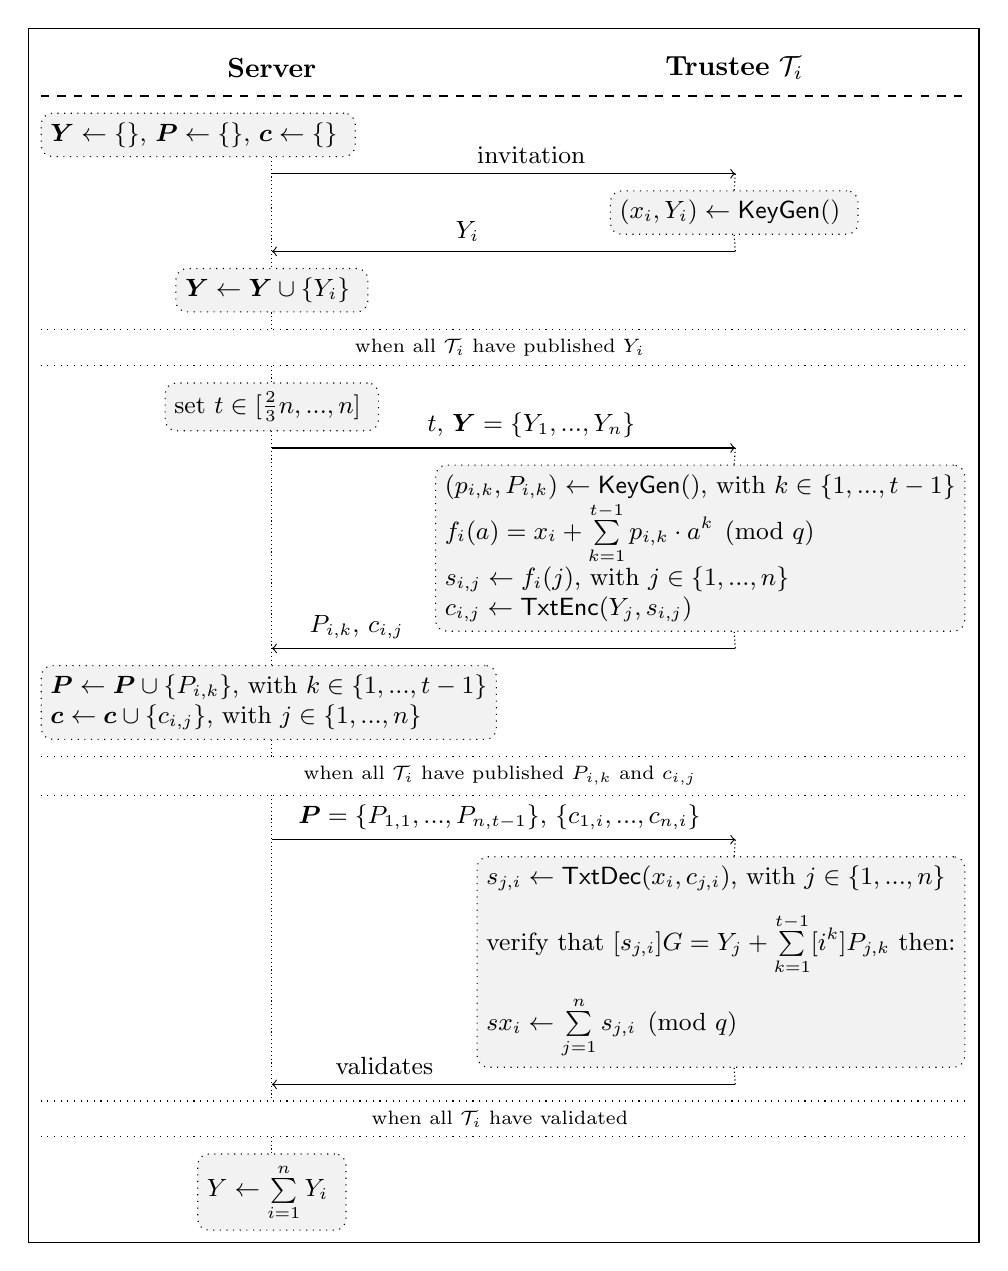
\begin{tikzpicture}[framed, node distance=0,
            spaced/.style={yshift=-6},
            % every node/.style={draw}
            ]{
            
        % Actors
        \node[title, above, anchor=north east] (s) {
            \textbf{Server}};
        \node[title, right=of s] (t) {
            \textbf{Trustee $\mathcal{T}_i$}};
        
        %All content
        \node[block, spaced, keep_left] at (s.south -| s.west) (s_1) {
            $\boldsymbol{Y} \gets \{ \}$, $\boldsymbol{P} \gets \{ \}$, $\boldsymbol{c} \gets \{ \}$
            };
        \node[arrow, towards_right, immediate, between={s.center}{t.center}] at (s_1.south -| s.south) (a_1) {
            \hspace{20pt} invitation
            };
        \node[block, spaced, keep_middle] at (a_1.south -| t.center) (t_1) {
            $(x_i, Y_i) \gets \mathsf{KeyGen}()$
            };
        \node[arrow, towards_left, immediate, between={s.center}{t.center}] at (t_1.south -| s.center) (a_2) {
            $Y_i$ \hspace{20pt}
            };
        \node[block, spaced, keep_middle] at (a_2.south -| s.center) (s_2) {
            $\boldsymbol{Y} \gets \boldsymbol{Y} \cup \{Y_i\}$
            };
        \node[banner, keep_left, spaced, between={s.west}{t.east}] at (s_2.south -| s.west) (b_1) {
            when all $\mathcal{T}_i$ have published $Y_i$
            };
        \node[block, keep_middle, spaced] at (b_1.south -| s.center) (s_3) {
            set $t \in [\frac{2}{3}n, ..., n]$
            };
        \node[arrow, towards_right, immediate, between={s.center}{t.center}] at (s_3.south -| s.center) (a_3) {
            \hspace{20pt} $t$, $\boldsymbol{Y} = \{Y_1, ..., Y_n\}$
            };
        \node[block, keep_right, spaced] at (a_3.south -| t.east) (t_2) {
            $(p_{i, k}, P_{i, k}) \gets \mathsf{KeyGen}()$, with $k \in \{1, ..., t-1\}$ \\
            $f_i(a) = x_i + \sum\limits_{k=1}^{t-1} p_{i, k} \cdot a^k \pmod q$ \\
            $s_{i, j} \gets f_i(j)$, with $j \in \{1, ..., n\}$ \\
            $c_{i, j} \gets \mathsf{TxtEnc} (Y_j, s_{i, j})$
            };
        \node[arrow, towards_left, immediate, between={s.center}{t.center}] at (t_2.south -| s.center) (a_4) {
            $P_{i, k}$, $c_{i, j}$ \hspace{100pt}
            };
        \node[block, keep_left, spaced] at (a_4.south -| s.west) (s_4) {
            $\boldsymbol{P} \gets \boldsymbol{P} \cup \{P_{i, k}\}$, with $k \in \{1, ..., t-1\}$ \\
            $\boldsymbol{c} \gets \boldsymbol{c} \cup \{c_{i, j}\}$, with $j \in \{1, ..., n\}$
            };
        \node[banner, keep_left, spaced, between={s.west}{t.east}] at (s_4.south -| s.west) (b_2) {
            when all $\mathcal{T}_i$ have published $P_{i, k}$ and $c_{i, j}$
            };
        \node[arrow, towards_right, between={s.center}{t.center}] at (b_2.south -| s.south) (a_5) {
            $\boldsymbol{P} = \{P_{1, 1}, ..., P_{n, t-1}\}$, $\{c_{1, i}, ..., c_{n, i}\}$
            };
        \node[block, keep_right, spaced] at (a_5.south -| t.east) (t_3) {
            $s_{j, i} \gets \mathsf{TxtDec} (x_i, c_{j, i})$, with $j \in \{1, ..., n\}$ \\ [7pt]
            verify that $[s_{j,i}]G = Y_j + \sum\limits_{k=1}^{t-1} [i^k]P_{j, k}$ then: \\ [7pt]
            $sx_i \gets \sum\limits_{j=1}^{n} s_{j, i} \pmod q$
            };
        \node[arrow, towards_left, immediate, between={s.center}{t.center}] at (t_3.south -| s.center) (a_6) {
            validates \hspace{80pt}
            };
        \node[banner, keep_left, spaced, between={s.west}{t.east}] at (a_6.south -| s.west) (b_3) {
            when all $\mathcal{T}_i$ have validated
            };
        \node[block, keep_middle, spaced] at (b_3.south -| s.center) (s_5) {
            $Y \gets \sum\limits_{i=1}^{n} Y_i$
            };
        
        % Arrows and lines
        \draw[dashed] (s.south west)--(t.south east);

        \draw[dotted] (b_1.north west)--(b_1.north east);
        \draw[dotted] (b_1.south west)--(b_1.south east);
        \draw[dotted] (b_2.north west)--(b_2.north east);
        \draw[dotted] (b_2.south west)--(b_2.south east);
        \draw[dotted] (b_3.north west)--(b_3.north east);
        \draw[dotted] (b_3.south west)--(b_3.south east);

        \draw[densely dotted] (s_1.south -| s.center)--(s_2.north -| s.center);
        \draw[densely dotted] (s_2.south -| s.center)--(b_1.north -| s.center);
        \draw[densely dotted] (b_1.south -| s.center)--(s_3.north -| s.center);
        \draw[densely dotted] (s_3.south -| s.center)--(s_4.north -| s.center);
        \draw[densely dotted] (s_4.south -| s.center)--(b_2.north -| s.center);
        \draw[densely dotted] (b_2.south -| s.center)--(b_3.north -| s.center);
        \draw[densely dotted] (b_3.south -| s.center)--(s_5.north -| s.center);

        \draw[densely dotted] (a_1.south east)--(t_1.north -| t.center);
        \draw[densely dotted] (t_1.south -| t.center)--(a_2.south east);
        \draw[densely dotted] (a_3.south east)--(t_2.north -| t.center);
        \draw[densely dotted] (t_2.south -| t.center)--(a_4.south east);
        \draw[densely dotted] (a_5.south east)--(t_3.north -| t.center);
        \draw[densely dotted] (t_3.south -| t.center)--(a_6.south east);
        }
    \end{tikzpicture}
    \caption{Threshold ceremony}
    \label{fig: threshold ceremony}
\end{figure}

At the end of the \textit{threshold ceremony}, for each trustee $\mathcal{T}_i$, with $i \in \{1, ..., n\}$, the \textit{public share of the decryption key} ($sY_i = [sx_i]G$) is publicly computable by the following:
\[
sY_i \gets \sum\limits_{j=1}^{n} (Y_j + \sum\limits_{k=1}^{t-1} [i^k]P_{j, k}).
\]

The encryption algorithm of the threshold cryptosystem is identical to the algorithm described in \cref{app: elgamal cryptosystem}:
\[
e = (R, C) \gets \mathsf{Enc}(Y, M; r).
\]

The decryption protocol of the threshold cryptosystem is inspired from paper \cite{Desmedt89}. At least $t$ trustees are needed to collaborate in the protocol described in \cref{fig: threshold decryption} in order to extract the message $M$ of a cryptogram $e = (R, C)$. We define $\tau \subset \{1, ..., n\}$ to be the subset of trustees that do participate in the decryption protocol, with $|\tau| \geq t$. 

Each trustee $\mathcal{T}_i$, with $i \in \tau$, computes a partial decryption $S_i \gets [sx_i]R$ and sends it to the server, where $sx_i$ is trustee's share of the decryption key. The trustee also publishes a proof of correct decryption in form of a non-interactive discrete logarithm zero knowledge proof $PK \gets \mathsf{DLProve} (sx_i, \{G, R\})$ (\cref{alg: dl prove}).

When receiving a partial decryption from a trustee $\mathcal{T}_i$, the server accepts it if the proof of correct decryption validates by $\mathsf{DLVer} (PK, \{G, R\}, \{sY_i, S_i\})$ (\cref{alg: dl ver}), where $sY_i$ is trustee's \textit{public share of the decryption key}.

After it received valid, partial decryptions from all trustees $\mathcal{T}_i$, with $i \in \tau$, the server aggregates all partial decryptions together to finalize the decryption and to output the message $M$. The aggregation process from \cite{Desmedt89} is described as follows:

Basically, $M = C - [x]R$, where $x$ is the main decryption key that nobody has. A possible way of computing $[x]R$ is by calculating the \textit{Lagrange Interpolation Polynomial} where each term is a partial decryption $S_i$ received from a trustee $\mathcal{T}_i$ that needs to be multiplied by the \textit{Lagrange Interpolation Polynomial coefficient} which is $\lambda(i) = \prod_{j \in \tau, j \neq i} \frac{-j}{i-j} \pmod q$. Formally,
\[
M \gets C - \sum_{i \in \tau} [\lambda(i)]S_i\text{, with } |\tau| \geq t .
\]

Note that the \textit{Lagrange Interpolation Polynomial} can be computed only when the number of terms is at least the degree of the polynomial, i.e $|\tau| \geq t$.

\begin{figure}[ht]
    \centering
    \begin{tikzpicture}[framed, node distance=0,
            spaced/.style={yshift=-6},
            % every node/.style={draw}
            ]{
            
        % Actors
        \node[title, above, anchor=north east] (s) {
            \textbf{Server}};
        \node[title, right=of s] (t) {
            \textbf{Trustee $\mathcal{T}_i$}};
            
        % internal knowledge
        \node[internal, below=of s] (s_ik) {
            internal knowledge: $e = (R, C)$, \\
            $\{sY_1, ..., sY_n\}$
            };
        \node[internal, below=of t] (t_ik) {
            internal knowledge: $sx_i$
            };
        
        %All content
        \node[block, keep_middle, spaced] at (s_ik.south -| s.center) (s_1) {
            $\tau \gets \{\}$
            };
        \node[arrow, towards_right, immediate, between={s.center}{t.center}] at (s_1.south -| s.center) (a_1) {
            \hspace{10pt} $e = (R, C)$
            };
        \node[block, keep_middle, spaced] at (a_1.south -| t.center) (t_1) {
            $S_i \gets [sx_i]R$ \\
            $PK \gets \mathsf{DLProve} (sx_i, \{G, R\})$
            };
        \node[arrow, towards_left, immediate, between={s.center}{t.center}] at (t_1.south -| s.center) (a_2) {
            $S_i$, $PK$ \hspace{50pt}
            };
        \node[block, keep_left, spaced] at (a_2.south -| s.west) (s_2) {
            verify $\mathsf{DLVer} (PK, \{G, R\}, \{sY_i, S_i\})$ then: \\ [7pt]
            $\tau \gets \tau \cup \{i\}$
            };
        \node[banner, keep_left, spaced, between={s.west}{t.east}] at (s_2.south -| s.west) (b_1) {
            when enough $\mathcal{T}_i$ have published $S_i$, i.e. $|\tau| \geq t$
            };
        \node[block, keep_left, spaced] at (b_1.south -| s.west) (s_3) {
            $\lambda(i) \gets \prod\limits_{j \in \tau, j \neq i} \frac{-j}{i-j} \pmod q$, with $i \in \tau$ \\
            $M \gets C - \sum_{i \in \tau} [\lambda(i)]S_i$
            };
        
        % Arrows and lines
        \draw[dashed] (s.south west)--(t.south east);
        \draw[dashed] (s_ik.south west)--(s_ik.south -| t_ik.east);

        \draw[dotted] (b_1.north west)--(b_1.north east);
        \draw[dotted] (b_1.south west)--(b_1.south east);

        \draw[densely dotted] (s_1.south -| s.center)--(s_2.north -| s.center);
        \draw[densely dotted] (s_2.south -| s.center)--(b_1.north -| s.center);
        \draw[densely dotted] (b_1.south -| s.center)--(s_3.north -| s.center);

        \draw[densely dotted] (a_1.south east)--(t_1.north -| t.center);
        \draw[densely dotted] (t_1.south -| t.center)--(a_2.south east);
        }
    \end{tikzpicture}
    \caption{Threshold decryption}
    \label{fig: threshold decryption}
\end{figure}

\clearpage
\subsubsection{Proving the Content of a Cryptogram} \label{app: proving the content of a cryptogram}
Once a cryptogram is generated $e = (R, C) \gets \mathsf{Enc} (Y, M; r)$, only the \textit{sender} (the one who generated the cryptogram) and the \textit{receiver} (the one in possession of the decryption key $x$) know the value of the message $M$. Both of them have the possibility to prove to somebody else (or publicly prove) the content of the cryptogram.

The one who generated the cryptogram can prove to a verifier that the cryptogram $e$ contains message $M$ by engaging in the protocol from \cref{fig: protocol for proving multiple discrete logarithms} in order to prove the knowledge of the randomizer $PK[(r): R = [r]G \wedge (C - M) = [r]Y]$. To generate a publicly verifiable proof, the \textit{sender} can generate a non-interactive proof $PK \gets \mathsf{DLProve} (r, \{G, Y\})$ (\cref{alg: dl prove}). Any public verifier is convinced that cryptogram $e$ contains message $M$ if the verification algorithm succeeds $\mathsf{DLVer} (PK, \{G, Y\}; \{R, C - M\})$ (\cref{alg: dl ver}).

At the same time, the one in possession of the decryption key $x$ can prove the content of the cryptogram $e$ to a verifier by engaging in the same protocol from \cref{fig: protocol for proving multiple discrete logarithms} but this time for proving the knowledge of the decryption key $PK[(x): Y = [x]G \wedge (C - M) = [x]R]$. To generate a publicly verifiable proof, the \textit{receiver} of the cryptogram can generate a non-interactive proof $PK \gets \mathsf{DLProve} (x, \{G, R\})$ (\cref{alg: dl prove}). Any public verifier is convinced that cryptogram $e$ contains message $M$ if the verification algorithm succeeds $\mathsf{DLVer} (PK, \{G, R\}; \{Y, C - M\})$ (\cref{alg: dl ver}).

\subsection{Schnorr digital signature}
The \textit{Schnorr digital signature scheme}, introduced in \cite{Schnorr90}, consists of a triple of algorithms (\textsf{KeyGen}, \textsf{Sign}, \textsf{SigVer}), which are based on elliptic curve cryptographic primitive.

A Schnorr key pair is a tuple $(x, Y) \gets \mathsf{KeyGen}()$ (\cref{alg: key gen}), where $x$ is the random, private signing key and $Y$ is the corresponding public signature verification key.

Only the owner of the signing key is able to generate a signature $\sigma = (c, s) \gets \mathsf{Sign} (x, m)$, on an arbitrary message $m \in \mathbb{B}^*$. In order to generate a signature, the signer follows \cref{alg: sign}.

\begin{algorithm}[ht]
    \DontPrintSemicolon
    \caption{$\mathsf{Sign} (x, m)$}
    \KwData{The signing key $x \in \mathbb{Z}_q$}
    \KwMoreData{The message to be signed $m \in \mathbb{B}^*$}
    
    $r \in_\mathrm{R} \mathbb{Z}_q$ \\
    $K \gets [r]G$ \\
    $c \gets \mathcal{H}(K || m)$ \\
    $s \gets r - c \cdot x \pmod q$ \\
    $\sigma \gets (c, s)$ \\
    \Return{$\sigma$} \tcp*{$\sigma \in \mathbb{Z}_q \times \mathbb{Z}_q$}
    
    \label{alg: sign}
\end{algorithm}

Given a signature $\sigma$ on a message $m$, anybody in the possession of the public verification key $Y$ is able to verify the validity of the signature $b \gets \mathsf{SigVer} (Y, \sigma; m)$, with $b \in \mathbb{B}$ which represents $true$ or $false$. The signature verification algorithm is described in \cref{alg: sig ver}.

\begin{algorithm}[H]
    \DontPrintSemicolon
    \caption{$\mathsf{SigVer} (Y, \sigma; m)$}
    \KwData{The signature verification key $Y \in \mathbb{P}$}
    \KwMoreData{The signature $\sigma = (c, s) \in \mathbb{Z}_q \times \mathbb{Z}_q$}
    \KwMoreData{The signed message $m \in \mathbb{B}^*$}
    
    $K \gets [s]G + [c]Y$ \\
    \eIf{$c = \mathcal{H}(K || m)$}{
        $b \gets 1$ \tcp*{signature is valid}
        }{
        $b \gets 0$ \tcp*{signature is invalid}
        }
    \Return{$b$} \tcp*{$b \in \mathbb{B}$}
    
    \label{alg: sig ver}
\end{algorithm}

\subsection{Pedersen commitment scheme}
A \textit{commitment scheme} consists of a tuple of algorithms ($\mathsf{Com}$, $\mathsf{ComVer}$) that enables a writer to commit to a specific message $m$ while keeping it secret. At a later point, if appropriate, the writer has the ability to open the commitment and reveal the committed message $m$. The \textit{Pedersen Commitment Scheme} is a randomized commitment scheme introduced in \cite{Pedersen91-commitment}. Later, the scheme has been updated in \cite{Bootle18} to enable commitment computation on a list of messages $\boldsymbol{m} = \{ m_1, ..., m_n \}$, where each $m_i \in \mathbb{Z}_q$, with $i \in \{ 1, ..., n \}$.

An important part of the commitment scheme is the existence of multiple generators (one for each message in the list  $\boldsymbol{m}$) in the subgroup such that the discrete logarithm amongst any two of them is unknown. To support that, we define the algorithm $\mathsf{BaseGen}$ that outputs a new generator $H$ such that the value $x$ is unknown where $H = [x]G$.

In order to commit to messages $\boldsymbol{m} = \{ m_1, ..., m_n \}$ a writer computes the commitment $C \gets \mathsf{Com}(\boldsymbol{m}; r)$ (\cref{alg: com}), where $r \in_\mathrm{R} \mathbb{Z}_q$ is a randomizer. The algorithm internally computes a list of generators $\boldsymbol{G} = \{ G_1, ..., G_n \}$ where each $G_i \gets \mathsf{BaseGen}(i)$ (\cref{alg: base gen}), with $i \in \{ 1, ..., n \}$.

In order to reveal messages $\boldsymbol{m}$, the writer needs to publish values $\boldsymbol{m}$ and $r$. A verifier is convinced that the commitment $C$ opens to messages $\boldsymbol{m}$ by running $b \gets \mathsf{ComVer}(C, \boldsymbol{m}; r)$ (\cref{alg: com ver}).

\begin{algorithm}[ht]
    \DontPrintSemicolon
    \caption{$\mathsf{BaseGen} (i)$}
    \KwData{An index $i \in \mathbb{N}$}
    
    $j \gets 0$ \\
    \Repeat{$H$ is valid}{
        $x \gets \mathcal{H}(G || i || j)$ \\
        $y \gets \mathsf{RecoverY}(x)$ \tcp*{according to elliptic curve equation}
        \If{$y$ is invalid}{
            $j \gets j + 1$ \;
            \Continue \;
        }
        $H \gets (x, y)$ \;
        \If{$H$ is invalid}{
            $j \gets j + 1$ \;
            \Continue \;
        }
    }
    \Return{$H$} \tcp*{$H \in \mathbb{P}$}
    
    \label{alg: base gen}
\end{algorithm}

\begin{algorithm}[ht]
    \DontPrintSemicolon
    \caption{$\mathsf{Com} (\boldsymbol{m}; r)$}
    \KwData{The list of messages $\boldsymbol{m} = \{ m_1, ..., m_n \} \in \mathbb{Z}_q^n$}
    \KwMoreData{The randomizer $r \in \mathbb{Z}_q$}
    
    \For{$i \gets 1$ \KwTo $n$ \KwBy $1$}{
        $G_i \gets \mathsf{BaseGen} (i)$
    }
    $C \gets [r]G + \sum\limits_{i=1}^n [m_i]G_i$ \;
    
    \Return{$C$} \tcp*{$C \in \mathbb{P}$}
    
    \label{alg: com}
\end{algorithm}

\begin{algorithm}[ht]
    \DontPrintSemicolon
    \caption{$\mathsf{ComVer} (C, \boldsymbol{m}; r)$}
    \KwData{The commitment $C \in \mathbb{P}$}
    \KwMoreData{The list of messages $\boldsymbol{m} = \{ m_1, ..., m_n \} \in \mathbb{Z}_q^n$}
    \KwMoreData{The randomizer $r \in \mathbb{Z}_q$}
    
    \For{$i \gets 1$ \KwTo $n$ \KwBy $1$}{
        $G_i \gets \mathsf{BaseGen} (i)$
    }
    \eIf{$C = [r]G + \sum\limits_{i=1}^n [m_i]G_i$}{
        $b \gets 1$ \tcp*{commitment is valid}
        }{
        $b \gets 0$ \tcp*{commitment is invalid}
        }
    \Return{$b$} \tcp*{$b \in \mathbb{B}$}
    
    \label{alg: com ver}
\end{algorithm}

\clearpage
\subsection{Groth's argument of shuffle} \label{app: groth's argument of shuffle}
A \textit{cryptographic shuffle} (or mixing) is a process that, given as input a list of cryptograms, outputs another list of cryptograms such that each cryptogram from the input list is re-encrypted and permuted in a random new order, forming the output list. This can be further extended to \textit{mixing} a matrix of cryptograms, where all cryptograms are re-encrypted and rows are permuted in a new order. Formally, given a matrix of cryptograms $\boldsymbol{e} = \{e_{1,1}, ..., e_{n,\ell}\} \in \mathbb{E}^{n,\ell}$, with each $e_{i,j} = (R_{i,j}, C_{i,j})$, $i \in \{1, ..., n\}$ and $j \in \{1, ..., \ell\}$, a matrix of randomizers $\boldsymbol{r} = \{r_{1,1}, ..., r_{n,\ell}\} \in \mathbb{Z}_q^{n \times \ell}$ and a permutation $\psi:\{1, ..., n\} \gets \{1, ..., n\}$ from the set $\Psi_n$ of all permutations of $n$ elements, the shuffle algorithm outputs the matrix $\boldsymbol{e'} = \{e'_{1,1}, ..., e'_{n,\ell}\} \gets \mathsf{Shuffle} (Y, \boldsymbol{e}; \boldsymbol{r}, \psi)$ (\cref{alg: shuffle}) where each $e'_{i,j} = (R'_{i,j}, C'_{i,j}) \gets \mathsf{ReEnc} (Y, e_{k,j}; r_{i,j})$ (\cref{alg: re enc}) for $k = \psi(i)$. 

\begin{algorithm}[ht]
    \DontPrintSemicolon
    \caption{$\mathsf{Shuffle}(Y, \boldsymbol{e}, \boldsymbol{r}, \psi)$}
    \KwData{The encryption key $Y \in \mathbb{P}$}
    \KwMoreData{The matrix of initial cryptograms $\boldsymbol{e} = \{e_{1,1}, ..., e_{n,\ell}\} \in \mathbb{E}^{n \times \ell}$}
    \KwMoreData{The matrix of randomizers $\boldsymbol{r} = \{r_{1,1}, ..., r_{n,\ell}\} \in \mathbb{Z}_q^{n \times \ell}$}
    \KwMoreData{The permutation $\psi \in \Psi_n$}
    
    \For{$i \gets 1$ \KwTo $n$ \KwBy $1$ }{
        \For{$j \gets 1$ \KwTo $\ell$ \KwBy $1$ }{
            $e'_{i,j} \gets \mathsf{ReEnc} (Y, e_{\psi(i),j}; r_{i,j})$ \tcp*{\cref{alg: re enc}}
            }
        }
    $\boldsymbol{e'} \gets \{e'_{1,1}, ..., e'_{n,\ell}\}$ \;
    \Return{$\boldsymbol{e'}$} \tcp*{$\boldsymbol{e'} \in \mathbb{E}^{n \times \ell}$}
    
    \label{alg: shuffle}
\end{algorithm}

The really interesting aspect of mixing is how to prove in zero knowledge that the shuffling calculations were done correctly and that no content of the cryptograms has been changed. Our mixing proof is based on an algorithm presented by Jens Groth in \cite{Groth05}. The proof uses as a building block an \textit{Argument for Shuffle of Known Contents} which is based on proving the knowledge of opening a commitment to a permutation of a set of known messages. The strategy of Groth's algorithm is to reduce the problem of proving that $\boldsymbol{e'}$ is the shuffled list of re-encrypted cryptograms $\boldsymbol{e}$ to the problem of proving the shuffling of some known messages where the same permutation $\psi$ is applied.

The protocol for the Argument of Shuffle of Known Contents is presented in \cref{fig: argument of shuffle of known contents protocol}. During this protocol, the \textit{Prover} convinces the \textit{Verifier} that $C$ is a commitment to a set of known messages $\boldsymbol{m} = \{m_1, ..., m_n\}$ that are shuffled by a secret permutation $\psi$. Note that, in this protocol, the \textit{Prover} does not reveal the permutation $\psi$.

The main protocol for proving the correctness of a shuffle is illustrated in \cref{fig: argument of shuffle of cryptograms protocol}. The \textit{Prover} convinces the \textit{Verifier} that the matrix of mixed cryptograms $\boldsymbol{e'} = \{e'_{1,1}, ..., e'_{n,\ell}\}$ is equivalent to the initial matrix of cryptograms $\boldsymbol{e} = \{e_{1,1}, ..., e_{n,\ell}\}$, where each cryptogram is re-encrypted and rows of the initial matrix are shuffled amongst each other. Note that, during mixing, the integrity of each row is preserved, i.e all columns of the matrix are shuffled by the same permutation. The protocol uses, as a building block, the protocol for the Argument of Shuffle of Known Contents, presented in \cref{fig: argument of shuffle of known contents protocol}.

Note that, in the description of the protocols, we abuse notation and define $\sum_{i=1}^n e_i = \mathsf{HomAdd}(e_1; \mathsf{HomAdd}(e_2; ... \mathsf{HomAdd}(e_{n-1}; e_n) ... ))$ as the homomorphic addition of multiple cryptograms, with each $e_i \in \mathbb{E}$.

\begin{figure}[ht]
    \centering
    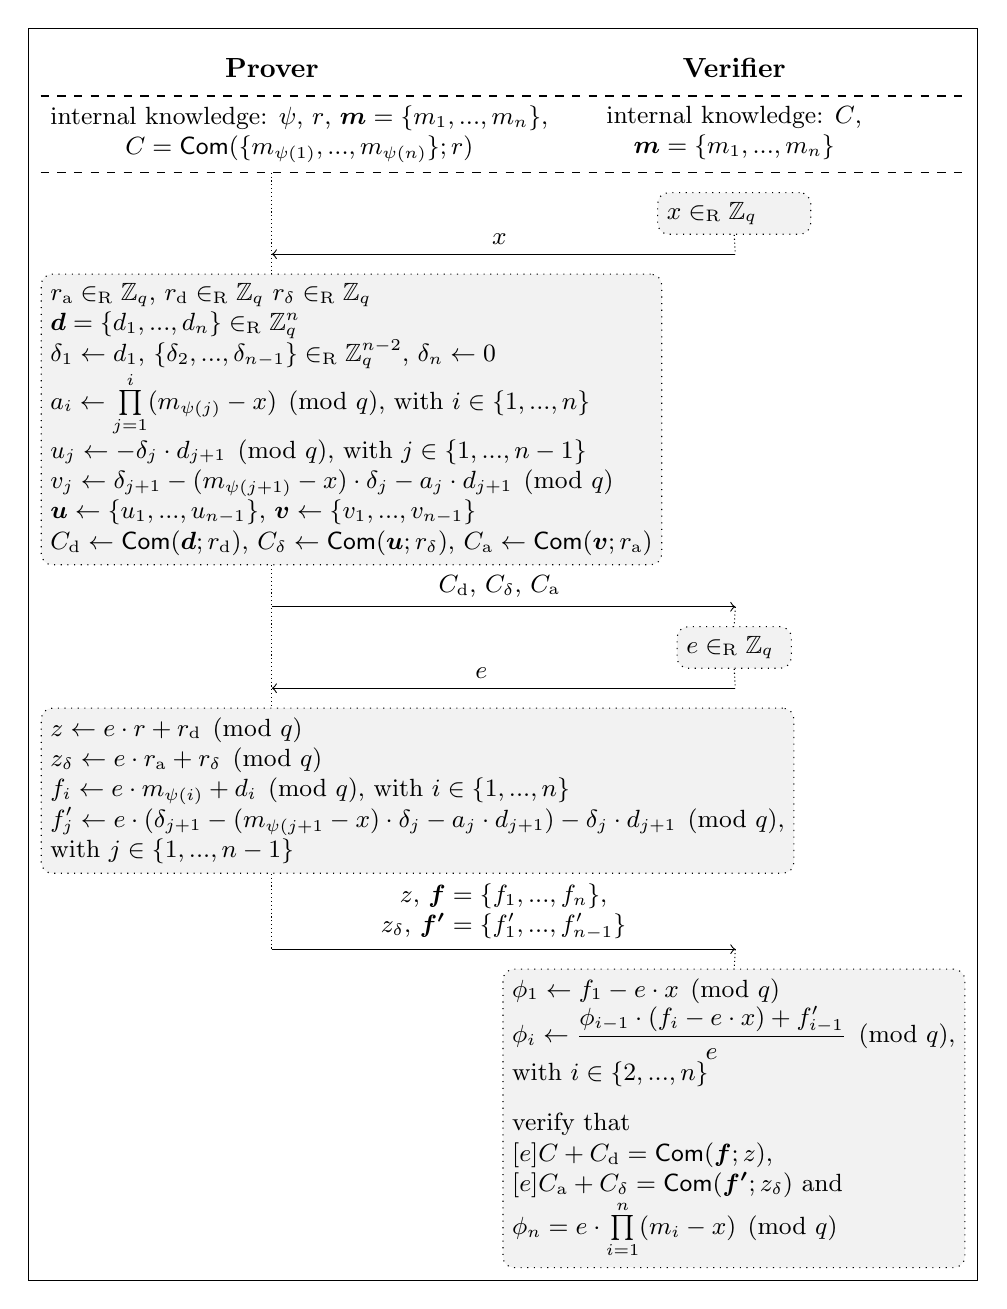
\begin{tikzpicture}[framed, node distance=0,
            % every node/.style={draw}
            ]{
            
        % Actors
        \node[title, above, anchor=north east] (p) {
            \textbf{Prover}};
        \node[title, right=of p] (v) {
            \textbf{Verifier}};
        
        % internal knowledge
        \node[ik, keep_left] at (p.south west) (p_ik) {
            internal knowledge: $\psi$, $r$, $\boldsymbol{m} = \{m_1, ..., m_n\}$, \\
            $C = \mathsf{Com} (\{m_{\psi(1)}, ..., m_{\psi(n)}\}; r)$
            };
        \node[ik] at (v.south) (v_ik) {
            internal knowledge: $C$, \\
            $\boldsymbol{m} = \{m_1, ..., m_n\}$
            };
        
        %All content
        \node[block, keep_middle, spaced] at (p_ik.south -| v.center) (v_1) {
            $x \in_\mathrm{R} \mathbb{Z}_q$ \hspace{10pt}
            };
        \node[arrow, towards_left, immediate, between={p.center}{v.center}] at (v_1.south -| p.center) (a_1) {
            $x$
            };
        \node[block, keep_left, spaced] at (a_1.south -| p.west) (p_1) {
            $r_\mathrm{a} \in_\mathrm{R} \mathbb{Z}_q$, $r_\mathrm{d} \in_\mathrm{R} \mathbb{Z}_q$ $r_\delta \in_\mathrm{R} \mathbb{Z}_q$ \\
            $\boldsymbol{d} = \{d_1, ..., d_n\} \in_\mathrm{R} \mathbb{Z}_q^n$ \\
            $\delta_1 \gets d_1$, $\{\delta_2, ..., \delta_{n-1}\} \in_\mathrm{R} \mathbb{Z}_q^{n-2}$, $\delta_n \gets 0$ \\
            $a_i \gets \prod\limits_{j=1}^i (m_{\psi(j)} - x) \pmod q$, with $i \in \{1, ..., n\}$ \\
            $u_j \gets -\delta_j \cdot d_{j+1} \pmod q$, with $j \in \{1, ..., n-1\}$ \\
            $v_j \gets \delta_{j+1} - (m_{\psi(j+1)} - x) \cdot \delta_j - a_{j} \cdot d_{j+1} \pmod q$ \\
            $\boldsymbol{u} \gets \{u_1, ..., u_{n-1}\}$, $\boldsymbol{v} \gets \{v_1, ..., v_{n-1}\}$ \\
            $C_\mathrm{d} \gets \mathsf{Com} (\boldsymbol{d}; r_\mathrm{d})$, $C_\delta \gets \mathsf{Com} (\boldsymbol{u}; r_\delta)$, $C_\mathrm{a} \gets \mathsf{Com} (\boldsymbol{v}; r_\mathrm{a})$
            };
        \node[arrow, towards_right, between={p.center}{v.center}] at (p_1.south -| p.center) (a_2) {
            $C_\mathrm{d}$, $C_\delta$, $C_\mathrm{a}$
            };
        \node[block, keep_middle, spaced] at (a_2.south -| v.center) (v_2) {
            $e \in_\mathrm{R} \mathbb{Z}_q$
            };
        \node[arrow, towards_left, immediate, between={p.center}{v.center}] at (v_2.south -| p.center) (a_3) {
            $e$ \hspace{10pt}
            };
        \node[block, keep_left, spaced] at (a_3.south -| p.west) (p_2) {
            $z \gets e \cdot r + r_\mathrm{d} \pmod q$ \\
            $z_\delta \gets e \cdot r_\mathrm{a} + r_\delta \pmod q$ \\
            $f_i \gets e \cdot m_{\psi(i)} + d_i \pmod q$, with $i \in \{1, ..., n\}$ \\
            $f'_j \gets e \cdot (\delta_{j+1} - (m_{\psi(j+1} -x) \cdot \delta_j - a_j \cdot d_{j+1}) - \delta_j \cdot d_{j+1} \pmod q$, \\
            with $j \in \{1, ..., n-1\}$
            };
        \node[arrow, towards_right, between={p.center}{v.center}] at (p_2.south -| p.center) (a_4) {
            $z$, $\boldsymbol{f} = \{f_1, ..., f_n\}$, \\
            $z_\delta$, $\boldsymbol{f'} = \{f'_1, ..., f'_{n-1}\}$
            };
        \node[block, keep_right, spaced] at (a_4.south -| v.east) (v_3) {
            $\phi_1 \gets f_1 - e\cdot x \pmod q$ \\
            $\phi_i \gets \dfrac{\phi_{i-1} \cdot (f_i - e \cdot x) + f'_{i-1}}{e} \pmod q$, \\
            with $i \in \{2, ..., n\}$ \\ [7pt]
            verify that \\
            $[e]C + C_\mathrm{d} = \mathsf{Com} (\boldsymbol{f}; z)$, \\
            $[e]C_\mathrm{a} + C_\delta = \mathsf{Com} (\boldsymbol{f'}; z_\delta)$ and \\
            $\phi_n = e \cdot \prod\limits_{i=1}^n (m_i - x) \pmod q$
            };
        
        % Arrows and lines
        \draw[dashed] (p.south west)--(v.south east);    
        \draw[dashed] (p_ik.south west)--(p_ik.south -| v.east);

        \draw[densely dotted] (p_ik.south -| p.center)--(p_1.north -| p.center);
        \draw[densely dotted] (p_1.south -| p.center)--(p_2.north -| p.center);
        \draw[densely dotted] (p_2.south -| p.center)--(a_4.south west);
        
        \draw[densely dotted] (v_1.south -| v.center)--(a_1.south east);
        \draw[densely dotted] (a_2.south east)--(v_2.north -| v.center);
        \draw[densely dotted] (v_2.south -| v.center)--(a_3.south east);
        \draw[densely dotted] (a_4.south east)--(v_3.north -| v.center);
        }
    \end{tikzpicture}
    \caption{Argument of Shuffle of Known Contents}
    \label{fig: argument of shuffle of known contents protocol}
\end{figure}

\begin{figure}[ht]
    \centering
    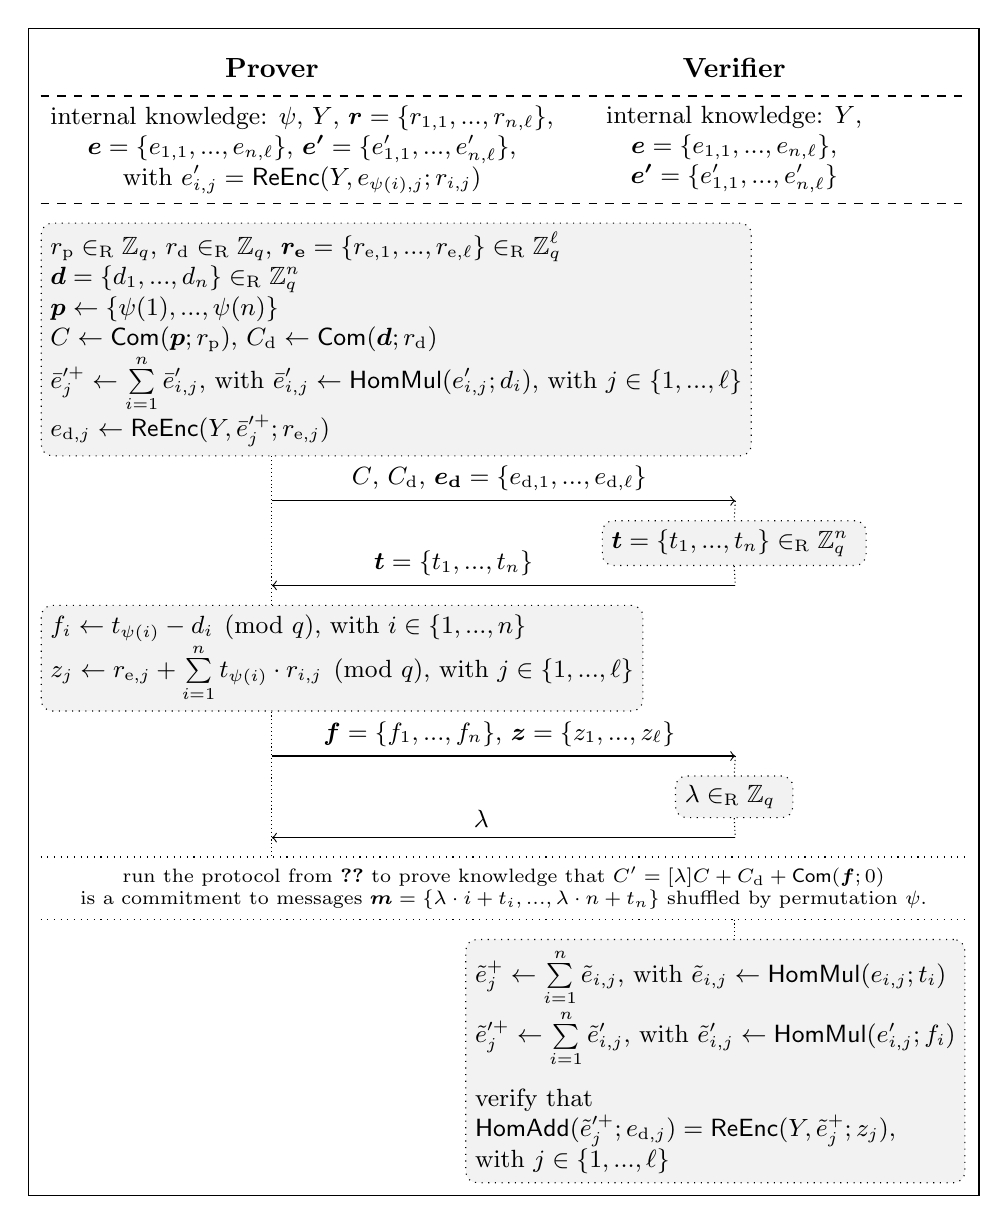
\begin{tikzpicture}[framed, node distance=0,
            % every node/.style={draw}
            ]{
            
        % Actors
        \node[title, above, anchor=north east] (p) {
            \textbf{Prover}};
        \node[title, right=of p] (v) {
            \textbf{Verifier}};
        
        % internal knowledge
        \node[ik, keep_left] at (p.south west) (p_ik) {
            internal knowledge: $\psi$, $Y$, $\boldsymbol{r} = \{r_{1,1}, ..., r_{n,\ell}\}$, \\
            $\boldsymbol{e} = \{e_{1,1}, ..., e_{n,\ell}\}$, $\boldsymbol{e'} = \{e'_{1,1}, ..., e'_{n,\ell}\}$, \\
            with $e'_{i,j} = \mathsf{ReEnc} (Y, e_{\psi(i),j}; r_{i,j})$
            };
        \node[ik] at (v.south) (v_ik) {
            internal knowledge: $Y$, \\
            $\boldsymbol{e} = \{e_{1,1}, ..., e_{n,\ell}\}$, \\
            $\boldsymbol{e'} = \{e'_{1,1}, ..., e'_{n,\ell}\}$
            };
        
        %All content
        \node[block, spaced, keep_left] at (p_ik.south -| p.west) (p_1) {
            $r_\mathrm{p} \in_\mathrm{R} \mathbb{Z}_q$, $r_\mathrm{d} \in_\mathrm{R} \mathbb{Z}_q$, $\boldsymbol{r_\mathrm{e}} = \{r_{\mathrm{e},1}, ..., r_{\mathrm{e},\ell}\} \in_\mathrm{R} \mathbb{Z}_q^\ell$ \\
            $\boldsymbol{d} = \{d_1, ..., d_n\} \in_\mathrm{R} \mathbb{Z}_q^n$ \\
            $\boldsymbol{p} \gets \{\psi(1), ..., \psi(n)\}$ \\
            $C \gets \mathsf{Com} (\boldsymbol{p}; r_\mathrm{p})$, $C_\mathrm{d} \gets \mathsf{Com} (\boldsymbol{d}; r_\mathrm{d})$ \\
            $\bar{e}_j^{\prime +} \gets \sum\limits_{i=1}^n \bar{e}'_{i,j}$, with $\bar{e}'_{i,j} \gets \mathsf{HomMul} (e'_{i,j}; d_i)$, with $j \in \{1, ..., \ell\}$ \\
            $e_{\mathrm{d},j} \gets \mathsf{ReEnc} (Y, \bar{e}_j^{\prime +};r_{\mathrm{e},j})$
            };
        \node[arrow, towards_right, between={p.center}{v.center}] at (p_1.south -| p.center) (a_1) {
            $C$, $C_\mathrm{d}$, $\boldsymbol{e_\mathrm{d}} = \{e_{\mathrm{d},1}, ..., e_{\mathrm{d},\ell}\}$
            };
        \node[block, keep_middle, spaced] at (a_1.south -| v.center) (v_1) {
            $\boldsymbol{t} = \{t_1, ..., t_n\} \in_\mathrm{R} \mathbb{Z}_q^n$
            };
        \node[arrow, towards_left, immediate, between={p.center}{v.center}] at (v_1.south -| p.center) (a_2) {
            $\boldsymbol{t} = \{t_1, ..., t_n\}$ \hspace{30pt}
            };
        \node[block, keep_left, spaced] at (a_2.south -| p.west) (p_2) {
            $f_i \gets t_{\psi(i)} - d_i \pmod q$, with $i \in \{1, ..., n\}$ \\
            $z_j \gets r_{\mathrm{e},j} + \sum\limits_{i=1}^n t_{\psi(i)} \cdot r_{i,j} \pmod q$, with $j \in \{1, ..., \ell\}$
            };
        \node[arrow, towards_right, between={p.center}{v.center}] at (p_2.south -| p.center) (a_3) {
            $\boldsymbol{f} = \{f_1, ..., f_n\}$, $\boldsymbol{z} = \{z_1, ..., z_\ell\}$
            };
        \node[block, keep_middle, spaced] at (a_3.south -| v.center) (v_2) {
            $\lambda \in_\mathrm{R} \mathbb{Z}_q$
            };
        \node[arrow, towards_left, immediate, between={p.center}{v.center}] at (v_2.south -| p.center) (a_4) {
            $\lambda$ \hspace{10pt}
            };
        \node[banner, keep_left, spaced, between={p.west}{v.east}] at (a_4.south -| p.west) (b_1) {
            run the protocol from \cref{fig: argument of shuffle of known contents protocol} to prove knowledge that $C' = [\lambda]C + C_\mathrm{d} + \mathsf{Com} (\boldsymbol{f}; 0)$ \\
            is a commitment to messages $\boldsymbol{m} = \{ \lambda \cdot i + t_i, ..., \lambda \cdot n + t_n \}$ shuffled by permutation $\psi$.
            };
        \node[block, keep_right, spaced] at (b_1.south -| v.east) (v_3) {
            $\tilde{e}_j^+ \gets \sum\limits_{i=1}^n \tilde{e}_{i,j}$, with $\tilde{e}_{i,j} \gets \mathsf{HomMul} (e_{i,j}; t_i)$ \\
            $\tilde{e}_j^{\prime +} \gets \sum\limits_{i=1}^n \tilde{e}'_{i,j}$, with $\tilde{e}'_{i,j} \gets \mathsf{HomMul} (e'_{i,j}; f_i)$ \\ [7pt]
            verify that \\
            $\mathsf{HomAdd} (\tilde{e}_j^{\prime +}; e_{\mathrm{d},j}) = \mathsf{ReEnc} (Y, \tilde{e}_j^+; z_j)$, \\
            with $j \in \{1, ..., \ell\}$
            };
        
        % Arrows and lines
        \draw[dashed] (p.south west)--(v.south east);    
        \draw[dashed] (p_ik.south west)--(p_ik.south -| v.east);

        \draw[dotted] (b_1.north west)--(b_1.north east);
        \draw[dotted] (b_1.south west)--(b_1.south east);

        \draw[densely dotted] (p_1.south -| p.center)--(p_2.north -| p.center);
        \draw[densely dotted] (p_2.south -| p.center)--(b_1.north -| p.center);

        \draw[densely dotted] (a_1.south east)--(v_1.north -| v.center);
        \draw[densely dotted] (v_1.south -| v.center)--(a_2.south east);
        \draw[densely dotted] (a_3.south east)--(v_2.north -| v.center);
        \draw[densely dotted] (v_2.south -| v.center)--(a_4.south east);
        \draw[densely dotted] (b_1.south -| v.center)--(v_3.north -| v.center);
        }
    \end{tikzpicture}
    \caption{Argument of Shuffle of Cryptograms}
    \label{fig: argument of shuffle of cryptograms protocol}
\end{figure}

Jens Groth suggests in \cite{Groth05} that the protocols can be turned into non-interactive algorithms by using the \textit{Fiat-Shamir heuristic} strategy \cite{Fiat87} to compute the random value $x$, $e$, $\boldsymbol{t}$ and $\lambda$ by applying a hash function to the transcript of the protocol.

Therefore, we transform each protocol into a set of two algorithms (one for generating a universally verifiable non-interactive proof and another for verifying it).

Explicitly, to prove the correct mixing of cryptograms $\boldsymbol{e} = \{e_{1,1}, ..., e_{n,\ell}\}$ by randomizers $\boldsymbol{r} = \{r_{1,1}, ..., r_{n,\ell}\}$ and permutation $\psi$ into the mixed cryptograms $\boldsymbol{e'} = \{e'_{1,1}, ..., e'_{n,\ell}\}$, the \textit{Prover} generates the tuple (proof of mixing and argument of shuffle) $(PM, AS) \gets \mathsf{ProveMix}(\psi, Y, \boldsymbol{r}, \boldsymbol{e}, \boldsymbol{e'})$ (\cref{alg: prove mix}), where $Y$ is the encryption key. Anybody can universally verify a proof of mixing by $\mathsf{VerMix}(PM, AS, Y, \boldsymbol{e}, \boldsymbol{e'})$ (\cref{alg: ver mix}).

\begin{algorithm}[ht]
    \DontPrintSemicolon
    \caption{$\mathsf{ProveASKC}(\psi; r; \boldsymbol{m}; C)$}
    \KwData{The permutation $\psi \in \Psi_n$}
    \KwMoreData{The randomizer $r \in \mathbb{Z}_q$}
    \KwMoreData{The list of known messages $\boldsymbol{m} = \{m_1, ..., m_n\} \in \mathbb{Z}_q^n$}
    \KwMoreData{The public commitment $C \in \mathbb{P}$}
    
    $x \gets \mathcal{H}(\boldsymbol{m} || C)$ \;
    $r_\mathrm{a} \in_\mathrm{R} \mathbb{Z}_q$, $r_\mathrm{d} \in_\mathrm{R} \mathbb{Z}_q$ $r_\delta \in_\mathrm{R} \mathbb{Z}_q$ \;
    \For{$i \gets 1$ \KwTo $n$ \KwBy $1$ }{
        $d_i \in_\mathrm{R} \mathbb{Z}_q$ \;
        $a_i \gets \prod\limits_{j=1}^i (m_{\psi(j)} - x) \pmod q$
        }
    $\delta_1 \gets d_1$, $\delta_n \gets 0$ \;
    \For{$i \gets 2$ \KwTo $n-1$ \KwBy $1$ }{
        $\delta_i \in_\mathrm{R} \mathbb{Z}_q$
        }
    \For{$i \gets 1$ \KwTo $n-1$ \KwBy $1$ }{
        $u_i \gets -\delta_i \cdot d_{i+1} \pmod q$ \;
        $v_i \gets \delta_{i+1} - (m_{\psi(i+1)} - x) \cdot \delta_i - a_{i} \cdot d_{i+1} \pmod q$
        }
    $\boldsymbol{d} \gets \{d_1, ..., d_n\}$, $\boldsymbol{u} \gets \{u_1, ..., u_{n-1}\}$, $\boldsymbol{v} \gets \{v_1, ..., v_{n-1}\}$ \;
    $C_\mathrm{d} \gets \mathsf{Com} (\boldsymbol{d}; r_\mathrm{d})$, $C_\delta \gets \mathsf{Com} (\boldsymbol{u}; r_\delta)$, $C_\mathrm{a} \gets \mathsf{Com} (\boldsymbol{v}; r_\mathrm{a})$ \;
    $e \gets \mathcal{H}(\boldsymbol{m} || C || C_\mathrm{d} || C_\delta || C_\mathrm{a})$ \;
    $z \gets e \cdot r + r_\mathrm{d} \pmod q$, $z_\delta \gets e \cdot r_\mathrm{a} + r_\delta \pmod q$ \;
    \For{$i \gets 1$ \KwTo $n$ \KwBy $1$ }{
        $f_i \gets e \cdot m_{\psi(i)} + d_i \pmod q$
        }
    \For{$i \gets 1$ \KwTo $n-1$ \KwBy $1$ }{
        $f'_i \gets e \cdot (\delta_{i+1} - (m_{\psi(i+1} -x) \cdot \delta_i - a_i \cdot d_{i+1}) - \delta_i \cdot d_{i+1} \pmod q$
        }
    $\boldsymbol{f} \gets \{f_1, ..., f_n\}$, $\boldsymbol{f'} \gets \{f'_1, ..., f'_{n-1}\}$ \;
    $AS \gets (C_\mathrm{d}, C_\delta, C_\mathrm{a}, x, e, z, z_\delta, \boldsymbol{f}, \boldsymbol{f'})$ \;
    
    \Return{$AS$} \tcp*{$AS \in \mathbb{P}^3 \times \mathbb{Z}_q^4 \times \mathbb{Z}_q^n \times \mathbb{Z}_q^{n-1}$}
    
    \label{alg: prove askc}
\end{algorithm}

\begin{algorithm}[ht]
    \DontPrintSemicolon
    \caption{$\mathsf{VerASKC}(AS; \boldsymbol{m}; C)$}
    \KwData{The argument $AS = (C_\mathrm{d}, C_\delta, C_\mathrm{a}, x, e, z, z_\delta, \boldsymbol{f}, \boldsymbol{f'}) \in \mathbb{P}^3 \times \mathbb{Z}_q^4 \times \mathbb{Z}_q^n \times \mathbb{Z}_q^{n-1}$}
    \KwMoreData{The list of known messages $\boldsymbol{m} = \{m_1, ..., m_n\} \in \mathbb{Z}_q^n$}
    \KwMoreData{The public commitment $C \in \mathbb{P}$}
    
    $\phi_1 \gets f_1 - e \cdot x \pmod q$ \;
    \For{$i \gets 2$ \KwTo $n$ \KwBy $1$ }{
        $\phi_i \gets \dfrac{\phi_{i-1} \cdot (f_i - e \cdot x) + f'_{i-1}}{e} \pmod q$   
        }
    \eIf{$x = \mathcal{H}(\boldsymbol{m} || C)$
    \KwAnd $e = \mathcal{H}(\boldsymbol{m} || C || C_\mathrm{d} || C_\delta || C_\mathrm{a})$ \\
    \KwAnd $[e]C + C_\mathrm{d} = \mathsf{Com}(\boldsymbol{f}; z)$
    \KwAnd $[e]C_\mathrm{a} + C_\delta = \mathsf{Com}(\boldsymbol{f'}; z_\delta)$ \\
    \KwAnd $\phi_n = e \cdot \prod\limits_{i=1}^n (m_i - x) \pmod q$}{
        $b \gets 1$ \tcp*{argument is valid}
        }{
        $b \gets 0$ \tcp*{argument is invalid}
        }
    
    \Return{$b$} \tcp*{$b \in \mathbb{B}$}
    
    \label{alg: ver askc}
\end{algorithm}

\begin{algorithm}[ht]
    \DontPrintSemicolon
    \caption{$\mathsf{ProveMix}(\psi, Y, \boldsymbol{r}, \boldsymbol{e}, \boldsymbol{e'})$}
    \KwData{The permutation $\psi \in \Psi_n$}
    \KwMoreData{The encryption key $Y \in \mathbb{P}$}
    \KwMoreData{The matrix of randomizers $\boldsymbol{r} = \{r_{1,1}, ..., r_{n,\ell}\} \in \mathbb{Z}_q^{n \times \ell}$}
    \KwMoreData{The matrix of initial cryptograms $\boldsymbol{e} = \{e_{1,1}, ..., e_{n,\ell}\} \in \mathbb{E}^{n \times \ell}$}
    \KwMoreData{The matrix of mixed cryptograms $\boldsymbol{e'} = \{e'_{1,1}, ..., e'_{n,\ell}\} \in \mathbb{E}^{n \times \ell}$, with}
    \KwMoreData{\hfill $e'_{i,j} = \mathsf{ReEnc}(Y, e_{\psi(i),j}; r_{i,j})$}
    
    $r_\mathrm{p} \in_\mathrm{R} \mathbb{Z}_q$, $r_\mathrm{d} \in_\mathrm{R} \mathbb{Z}_q$ \;
    \For{$i \gets 1$ \KwTo $n$ \KwBy $1$ }{
        $d_i \in_\mathrm{R} \mathbb{Z}_q$, $p_i \gets \psi(i)$ \;
        \For{$j \gets 1$ \KwTo $\ell$ \KwBy $1$ }{
            $\bar{e}'_{i,j} \gets \mathsf{HomMul} (e'_{i,j}; d_i)$ \tcp*{\cref{alg: hom mul}}
            }
        }
    $\boldsymbol{d} \gets \{d_1, ..., d_n\}$, $\boldsymbol{p} \gets \{p_1, ..., p_n\}$ \;
    $C \gets \mathsf{Com} (\boldsymbol{p}; r_\mathrm{p})$, $C_\mathrm{d} \gets \mathsf{Com} (\boldsymbol{d}; r_\mathrm{d})$ \tcp*{\cref{alg: com}}
    \For{$j \gets 1$ \KwTo $\ell$ \KwBy $1$ }{
        $r_{\mathrm{e},j} \in_\mathrm{R} \mathbb{Z}_q$ \;
        $e_{\mathrm{d},j} \gets \mathsf{ReEnc} (Y, \bar{e}_j^{\prime +};r_{\mathrm{e},j})$, with $\bar{e}_j^{\prime +} \gets \sum\limits_{i=1}^n \bar{e}'_{i,j}$ \tcp*{\cref{alg: re enc}}
        }
    $\boldsymbol{e_\mathrm{d}} \gets \{e_{\mathrm{d},1}, ..., e_{\mathrm{d},\ell}\}$ \;
    \For{$i \gets 1$ \KwTo $n$ \KwBy $1$ }{
        $t_i \gets \mathcal{H}(\boldsymbol{e} || \boldsymbol{e'} || C || C_\mathrm{d} || \boldsymbol{e_\mathrm{d}} || i)$
        }
    \For{$i \gets 1$ \KwTo $n$ \KwBy $1$ }{
        $f_i \gets t_{\psi(i)} - d_i \pmod q$
        }
    $\boldsymbol{f} \gets \{f_1, ..., f_n\}$ \;
    \For{$j \gets 1$ \KwTo $\ell$ \KwBy $1$ }{
        $z_j \gets r_{\mathrm{e},j} + \sum\limits_{i=1}^n t_{\psi(i)} \cdot r_{i,j} \pmod q$
        }
    $\boldsymbol{z} \gets \{z_1, ..., z_\ell\}$ \;
    $\lambda \gets \mathcal{H}(\boldsymbol{e} || \boldsymbol{e'} || C || C_\mathrm{d} || e_\mathrm{d} || \boldsymbol{f} || \boldsymbol{z})$ \;
    \For{$i \gets 1$ \KwTo $n$ \KwBy $1$ }{
        $m'_i \gets \lambda \cdot \psi(i) + t_{\psi(i)}$
        }
    $\boldsymbol{m'} \gets \{m'_1, ..., m'_n\}$, $r' \gets \lambda + r_\mathrm{d} \pmod{q}$ \;
    $C' \gets \mathsf{Com}(\boldsymbol{m'}; r')$ \tcp*{\cref{alg: com}}
    $AS \gets \mathsf{ProveASKC}(\psi; r'; \boldsymbol{m'}; C')$ \tcp*{\cref{alg: prove askc}}
    $PM \gets (C, C_\mathrm{d}, \boldsymbol{e_\mathrm{d}}, \boldsymbol{t}, \boldsymbol{f}, \boldsymbol{z}, \lambda)$
    
    \Return{$(PM, AS)$} \tcp*{
    $PM \in \mathbb{P}^2 \times \mathbb{E}^\ell \times \mathbb{Z}_q^{2n} \times \mathbb{Z}_q^\ell \times \mathbb{Z}_q$ \\
    $AS \in \mathbb{P}^3 \times \mathbb{Z}_q^4 \times \mathbb{Z}_q^n \times \mathbb{Z}_q^{n-1}$ \phantom{..}}
    
    \label{alg: prove mix}
\end{algorithm}

\begin{algorithm}[ht]
    \DontPrintSemicolon
    \caption{$\mathsf{VerMix}(PM, AS, Y, \boldsymbol{e}, \boldsymbol{e'})$}
    \KwData{The proof $PM = (C, C_\mathrm{d}, \boldsymbol{e_\mathrm{d}}, \boldsymbol{t}, \boldsymbol{f}, \boldsymbol{z}, \lambda) \in \mathbb{P}^2 \times \mathbb{E}^\ell \times \mathbb{Z}_q^{2n} \times \mathbb{Z}_q^\ell \times \mathbb{Z}_q$}
    \KwMoreData{The argument of shuffle $AS \in \times \mathbb{P}^3 \times \mathbb{Z}_q^4 \times \mathbb{Z}_q^n \times \mathbb{Z}_q^{n-1}$}
    \KwMoreData{The encryption key $Y \in \mathbb{P}$}
    \KwMoreData{The matrix of initial cryptograms $\boldsymbol{e} = \{e_{1,1}, ..., e_{n,\ell}\} \in \mathbb{E}^{n \times \ell}$}
    \KwMoreData{The matrix of mixed cryptograms $\boldsymbol{e'} = \{e'_{1,1}, ..., e'_{n,\ell}\} \in \mathbb{E}^{n \times \ell}$}
    
    \For{$i \gets 1$ \KwTo $n$ \KwBy $1$ }{
        \For{$j \gets 1$ \KwTo $\ell$ \KwBy $1$ }{
            $\tilde{e}_{i,j} \gets \mathsf{HomMul}(e_{i,j}; t_i)$ \tcp*{\cref{alg: hom mul}}
            $\tilde{e}'_{i,j} \gets \mathsf{HomMul}(e'_{i,j}; f_i)$ \tcp*{\cref{alg: hom mul}}
        }
        $m_i \gets \lambda \cdot i + t_i \pmod q$
        }
    \For{$j \gets 1$ \KwTo $\ell$ \KwBy $1$ }{
        $\tilde{e}_j^+ \gets \sum\limits_{i=1}^n \tilde{e}_{i,j}$ \;
        $\tilde{e}_j^{\prime +} \gets \sum\limits_{i=1}^n \tilde{e}'_{i,j}$ \;
        }
    $C' \gets [\lambda]C + C_\mathrm{d} + \mathsf{Com}(\boldsymbol{f}; 0)$ \;
    $\boldsymbol{m} \gets \{m_1, ..., m_n\}$ \tcp*{\cref{alg: com}}
    \eIf{$t_i = \mathcal{H}(\boldsymbol{e} || \boldsymbol{e'} || C || C_\mathrm{d} || \boldsymbol{e_\mathrm{d}} || i)$, where $i \in \{1, ..., n\}$ \\
    \KwAnd $\lambda = \mathcal{H}(\boldsymbol{e} || \boldsymbol{e'} || C || C_\mathrm{d} || \boldsymbol{e_\mathrm{d}} || \boldsymbol{f} || \boldsymbol{z})$ \\
    \KwAnd $\mathsf{HomAdd}(\tilde{e}_j^{\prime +}; e_{\mathrm{d},j}) = \mathsf{ReEnc}(Y, \tilde{e}_j^+; z_j)$
    , where $j \in \{1, ..., \ell\}$ \\
    \KwAnd $\mathsf{VerASKC}(AS; \boldsymbol{m}; C')$ \tcp*{\cref{alg: ver askc}}}{
        $b \gets 1$ \tcp*{proof is valid}
        }{
        $b \gets 0$ \tcp*{proof is invalid}
        }
    
    \Return{$b$} \tcp*{$b \in \mathbb{B}$}
    
    \label{alg: ver mix}
\end{algorithm}

\clearpage
\subsection{Key derivation} \label{app: key derivation}
Key derivation functions are algorithms that convert one source of randomness and secrecy (such as private keys or passwords) into different formats that can be used in different applications.


\subsubsection{Password-based key derivation function} \label{app: password-based key derivation function}
$\mathsf{PBKDF2}$ is a standard algorithm, described in \cite{RFC8018}, that converts passwords (arbitrary text) into keys that can be used in a cryptographic context. The algorithm takes as arguments a pseudorandom function, a password, a salt, an iteration count, and the desired length of the output key in bytes.

We use $\mathsf{PBKDF2}$ as a building block for $\mathsf{Pass2Key}(m)$ (\cref{alg: pass to key}) that converts password $m$ into a key pair $(x, Y)$. This can be seen as an alternative algorithm to $\mathsf{KeyGen}()$ (\cref{alg: key gen}) that can be used to get a deterministic key pair based on some random seed.

Particularly, no salt is used (i.e., salt is set to $\varnothing$), therefore, only one key pair can be derived from password $m$. The amount of iterations is set to 600.000, according to recommendations from \cite{OWASP}. The password is concatenated with a counter that gets incremented until the output of the key derivation function can be interpreted as a correct private key (i.e., the output bytes are decoded as integer $x$, then checked whether $x \in \mathbb{Z}_q$).

\begin{algorithm}[ht]
    \DontPrintSemicolon
    \caption{$\mathsf{Pass2Key}(m)$}
    \label{alg: pass to key}
    \KwData{A text $m \in \mathbb{B}^*$}
    
    $salt \gets \varnothing$ \;
    $iterations \gets 600.000$ \;
    $\ell \gets \mathsf{ByteLengthOf}(q)$ \tcp*{\cref{alg: bytes length of}}
    $i \gets 0$ \;
    \Repeat{$x < q$}{
        $x \gets \mathsf{PBKDF2}(\mathcal{H}, m || i, salt, iterations, \ell)$ \\
        \If{$x \geq q$}{
            $i \gets i + 1$ \;
            \Continue \;
        }
    }
    $Y \gets [x]G$ \;
    \Return{$(x, Y)$} \tcp*{$(x, Y) \in \mathbb{Z}_q \times \mathbb{P}$}
\end{algorithm}


\clearpage
\subsubsection{Diffie Hellman key derivation function} \label{app: diffie hellman key derivation function}
To use symmetric encryption for encrypting arbitrary amounts of data, a symmetric key needs to be derived from a private-public key environment. Algorithm $\mathsf{DerSymKey}(x_1, Y_2)$ (\cref{alg: der sym key}) deterministically computes a 256-bit symmetric key $k \in \mathbb{B}^{256}$, given a private key and a public key that are not related (i.e., $Y_2 \neq [x_1]G$).

For two entities that have a private-public key infrastructure in place (i.e., entity 1 has key pair $(x_1, Y_1)$ and entity 2 has key pair $(x_2, Y_2)$, where $Y_1 = [x_1]G$ and $Y_2 = [x_2]G$) and that know each other (i.e., entity 1 knows $Y_2$ and entity 2 knows $Y_1$), they can both derive symmetric key $k$ by running $\mathsf{DerSymKey}(x_1, Y_2)$ as entity 1 and $\mathsf{DerSymKey}(x_2, Y_1)$ as entity 2.

The algorithm performs a Diffie Hellman key exchange to reach a shared secret $S \gets [x_1]Y_2 = [x_2]Y_1 = [x_1 + x_2]G$. The resulting value is used as the keying material of a hash-based key derivation function $\mathsf{HKDF}$ (described in \cite{RFC5869}) to convert it into a uniform key $k$. Particularly, no salt and info arguments are used (i.e., salt and info are set to $\varnothing$), therefore only one symmetric key can be derived from two particular key pairs $(x_1, Y_1)$ and $(x_2, Y_2)$.

\begin{algorithm}[ht]
    \DontPrintSemicolon
    \caption{$\mathsf{DerSymKey}(x, Y)$}
    \label{alg: der sym key}
    \KwData{A private key $x \in \mathbb{Z}_q$}
    \KwMoreData{A public key $Y \in \mathbb{P}$}
    
    $salt \gets \varnothing$ \;
    $info \gets \varnothing$ \;
    $length \gets 256$ \;
    $S \gets [x]Y$ \;
    $k \gets \mathsf{HKDF}(S, salt, info, length)$ \;
    \Return{$k$} \tcp*{$k \in \mathbb{B}^{256}$}
\end{algorithm}

\clearpage
\begin{landscape}
\section{Bulletin board item types} \label{app: bulletin board item types}

All item types that can appear on the bulletin board are described in the following list and are grouped in the following 3 categories:

\paragraph{Configuration items}
\begin{longtable}{|
        >{\raggedright}p{\dimexpr0.13\linewidth-2\tabcolsep} |
        >{\centering}p{\dimexpr0.09\linewidth-2\tabcolsep} |
        >{\raggedright}p{\dimexpr0.30\linewidth-2\tabcolsep} |
        >{\raggedright}p{\dimexpr0.13\linewidth-2\tabcolsep} |
        p{\dimexpr0.35\linewidth-2\tabcolsep} |
    } 
    \hline
    \textbf{Item} &
    \textbf{Writer} &
    \textbf{Content} &
    \textbf{Parent type} &
    \textbf{Validation rules} \\
    \hline
    \endhead

    genesis &
    $\mathcal{D}$ &
    elliptic curve domain parameters $(p, a, b, G, q, h)$, \newline digital ballot box public key $Y_\mathcal{D}$, \newline election admin public key $Y_\mathcal{E}$ &
    none & 
    It is the first item of the board.
    \\ \hline

    election configuration &
    $\mathcal{E}$ &
    election title, \newline enabled languages &
    latest configuration item &
    The first item defines the configuration. \newline The following items update the configuration.
    \\ \hline

    contest configuration &
    $\mathcal{E}$ &
    contest identifier, \newline contest marking rules, question type and result rules, \newline candidate labels $\{m_1, ..., m_{n_\mathrm{c}}\}$ &
    latest configuration item &
    The first item with a contest identifier defines the configuration of that contest. \newline The following items with the same contest identifier update the configuration of that specific contest.
    \\ \hline

    threshold configuration &
    $\mathcal{E}$ &
    ballot encryption key $Y_\mathrm{enc}$, \newline threshold setup $t$ out-of $n_\mathrm{t}$, \newline trustees public keys $\{Y_{\mathcal{T}_1}, ..., Y_{\mathcal{T}_{n_\mathrm{t}}}\}$, \newline trustees public polynomial coefficients $\{P_{\mathcal{T}_1, 1}, ..., P_{\mathcal{T}_{n_\mathrm{t}}, t-1}\}$ &
    latest configuration item &
    This item cannot be updated.
    \\ \hline

    actor configuration &
    $\mathcal{E}$ &
    actor identifier, \newline actor role, \newline actor public key &
    latest configuration item &
    The first item with an actor identifier defines the configuration of that actor. \newline The following items with the same actor identifier update the configuration of that specific actor. \newline The roles can be: \textit{Voter Authorizer} $\mathcal{A}$ and \textit{Ballot Adjudicator} $\mathcal{B}$.
    \\ \hline

    voter authorization configuration &
    $\mathcal{A}$ &
    the voter authorization mode, \newline configuration of all Identity Providers $\{\mathcal{I}_1, ..., \mathcal{I}_{n_\mathrm{i}}\}$ &
    latest configuration item &
    The first item defines the voter authorization configuration. \newline The following items update the configuration. \newline The configuration of Identity Providers is included only if voter authorization mode is \textbf{on-demand}.
    \\ \hline

    voting round &
    $\mathcal{E}$ &
    voting round identifier, \newline start date and end date, \newline list of enabled contest identifiers &
    latest configuration item &
    The first item with a voting round identifier defines the configuration of that voting round. \newline The following items with the same voting round identifier update the configuration of that specific voting round.
    \\ \hline
\end{longtable}

\clearpage
\paragraph{Voting items}
\begin{longtable}{|
    >{\raggedright}p{\dimexpr0.13\linewidth-2\tabcolsep} |
    >{\centering}p{\dimexpr0.09\linewidth-2\tabcolsep} |
    >{\raggedright}p{\dimexpr0.30\linewidth-2\tabcolsep} |
    >{\raggedright}p{\dimexpr0.13\linewidth-2\tabcolsep} |
    p{\dimexpr0.35\linewidth-2\tabcolsep} |
} 
    \hline
    \textbf{Item} &
    \textbf{Writer} &
    \textbf{Content} &
    \textbf{Parent type} &
    \textbf{Validation rules} \\
    \hline
    \endhead

    voter session &
    $\mathcal{A}$ &
    voter identifier, \newline voter's public key $Y_i$, \newline voter's weight, \newline voter's authentication fingerprint \newline list of assigned contest identifiers &
    latest configuration item &
    This item can be created only during the election phase. \newline The following voter session items with the same voter identifier overwrite the previous voter sessions of that voter.
    \\ \hline

    voter encryption commitment &
    $\mathcal{V}_i$ &
    commitment $c_\mathrm{v}$ &
    the voter session item &
    Voter's public key $Y_i$ is defined in the voter session item.
    \\ \hline

    server encryption commitment &
    $\mathcal{D}$ &
    commitment $c_\mathrm{d}$ &
    the voter encryption commitment item &
    There can be only one server encryption commitment item referencing the voter encryption commitment item. \newline This item is created as a response to the voter encryption commitment item being created.
    \\ \hline

    ballot cryptograms &
    $\mathcal{V}_i$ &
    cryptogram $e_i$ &
    the server encryption commitment item &
    There can be only one ballot cryptograms item referencing the server encryption commitment item. \newline Voter's public key $Y_i$ is defined in the voter session item.
    \\ \hline

    cast request &
    $\mathcal{V}_i$ &
    &
    the ballot cryptograms item &
    There can be either a cast request or a spoil request item referencing the ballot cryptograms item. \newline Voter's public key $Y_i$ is defined in the voter session item.
    \\ \hline

    spoil request &
    $\mathcal{V}_i$ &
    &
    the ballot cryptograms item &
    There can be either a cast request or a spoil request item referencing the ballot cryptograms item. \newline Voter's public key $Y_i$ is defined in the voter session item.
    \\ \hline
    
    ballot accepted &
    $\mathcal{B}$ &
    &
    the cast request item or a ballot rejected item &
    \\ \hline

    ballot rejected &
    $\mathcal{B}$ &
    rejection reason &
    the cast request item or a ballot accepted item &
    \\ \hline
\end{longtable}

\clearpage
\paragraph{Hidden items}
\begin{longtable}{|
    >{\raggedright}p{\dimexpr0.13\linewidth-2\tabcolsep} |
    >{\centering}p{\dimexpr0.09\linewidth-2\tabcolsep} |
    >{\raggedright}p{\dimexpr0.30\linewidth-2\tabcolsep} |
    >{\raggedright}p{\dimexpr0.13\linewidth-2\tabcolsep} |
    p{\dimexpr0.35\linewidth-2\tabcolsep} |
}
    \hline
    \textbf{Item} &
    \textbf{Writer} &
    \textbf{Content} &
    \textbf{Parent type} &
    \textbf{Validation rules} \\
    \hline
    \endhead

    verification track start &
    $\mathcal{D}$ &
    &
    the ballot cryptograms item &
    There can be only one verification track start item referencing the ballot cryptograms item. \newline This item is created as a response to the ballot cryptograms item being created.
    \\ \hline

    verifier &
    $\mathcal{X}$ &
    external verifier's public key $Y_\mathcal{X}$ &
    the verification track start item &
    This is a self signed item, i.e. the public key of the author is defined in the item itself. \newline There can be only one verifier item referencing the verifiaction track start item.
    \\ \hline

    voter commitment opening &
    $\mathcal{V}_i$ &
    encrypted commitment opening $d_\mathrm{v}$ &
    the verifier item &
    There can be only one voter commitment opening item referencing the verifier item.
    \\ \hline

    server commitment opening &
    $\mathcal{D}$ &
    encrypted commitment opening $d_\mathrm{d}$ &
    the voter commitment opening item &
    There can be only one server commitment opening item referencing the voter commitment opening item.
    \\ \hline
\end{longtable}

\clearpage
\paragraph{Result items}
\begin{longtable}{|
    >{\raggedright}p{\dimexpr0.13\linewidth-2\tabcolsep} |
    >{\centering}p{\dimexpr0.09\linewidth-2\tabcolsep} |
    >{\raggedright}p{\dimexpr0.30\linewidth-2\tabcolsep} |
    >{\raggedright}p{\dimexpr0.13\linewidth-2\tabcolsep} |
    p{\dimexpr0.35\linewidth-2\tabcolsep} |
} 
    \hline
    \textbf{Item} &
    \textbf{Writer} &
    \textbf{Content} &
    \textbf{Parent type} &
    \textbf{Validation rules} \\
    \hline
    \endhead

    extraction intent &
    $\mathcal{E}$ &
    &
    latest config item &
    \\ \hline

    extraction data &
    $\mathcal{D}$ &
    a fingerprint of list of cryptograms $\boldsymbol{e}_0$ &
    the extraction intent item &
    There can be a single extraction data item referencing the extraction intent item. \newline The item provides a way of aquiring the list $\boldsymbol{e}_0 = \{ e_1, ..., e_{n_\mathrm{e}} \}$.
    \\ \hline

    extraction confirmation &
    $\mathcal{E}$ &
    list of trustees that participated in the result ceremony $\boldsymbol{\mathcal{T}'}$, \newline fingerprints of each intermediate mixed boards of cryptograms $\boldsymbol{e}_i$ and proofs of correct mixing $(PM_i, AS_i)$, \newline fingerprints of each partial decryption $\boldsymbol{S}_i$ and proofs of correct decryption $PK_i$, \newline signatures from each trustee $\mathcal{T}_i \in \boldsymbol{\mathcal{T}'}$ on all the fingerprints above &
    the extraction data item &
    There can be only one extraction confirmation item referencing the extraction data item.
    \\ \hline
\end{longtable}
\end{landscape}

\clearpage
\section{Extra features} \label{app: extra features}

\subsection{Affidavit document extension} \label{app: affidavit document extension}
The affidavit document extension is an optional feature that includes an extra authentication factor in form of an affidavit that is hand signed by the voter. The affidavit accompanies the encrypted digital ballot.


\subsubsection{General description}
The affidavit feature is an extra verifiability check that is implemented upon the election phase when a \textit{Voter} $\mathcal{V}_i$ wants to submit his vote as described in \cref{sec: election phase} (bullet point 3) then an additional step is required by the user which is to provide a signed affidavit to the voting application. During the election phase, after a voter has submitted his vote and an affidavit, the affidavit is manually checked by an \textit{Election Administrator} $\mathcal{E}$ who then either accept or rejects the signature. In the post-election phase only cryptograms that are accompanied by accepted affidavits will pass through the cleansing phase to be part of the mixing and decryption phases as described in \cref{sec: cleansing procedure}.

The file is then encrypted with the encryption key $Y_\mathrm{aff}$ that is written from the election configuration. The file is encrypted using symmetric encryption as described in (ref to symmetric algorithm) where it is also described how $Y_\mathrm{aff}$ is transformed into a symmetric key.

The encrypted affidavit is then sent to the \textit{Digital Ballot Box} $\mathcal{D}$ and stored encrypted privately by the \textit{Digital Ballot Box} $\mathcal{D}$ and a fingerprint of the encrypted affidavit is posted on the bulletin board together with the vote cryptogram. This also means that the affidavit extension modifies the cast-request item described in \cref{sec: writing on the bulletin board} as the item now contains a field with this aforementioned fingerprint.


The affidavit is verified as being genuine, that is generated in a appropriate voting application, by (what parameter?). After being verified the affidavit is unencrypted and the contents are manually accepted or rejected by an \textit{Election Administrator} $\mathcal{E}$.

During the affi davit process an id is generated for the user $\mathcal{V}_{{F}_i}$ which the \textit{Election Administrator} $\mathcal{E}$ then uploads after the affi davit is submitted.


\subsubsection{How it impacts our protocol}
In the pre-election phase the \textit{Election Administrator} $\mathcal{E}$ has to generate an asymmetric key pair for the encryption and decryption of the affidavits. \( (x_\mathrm{aff}, Y_{\mathcal{E}_f}) \leftarrow \mathsf{KeyGen}() \) (\cref{alg: key gen}), where $x_{\mathcal{E}_f}$ is the private key and will be kept private by the \textit{Election Administrator} $\mathcal{E}$, and $Y_{\mathcal{E}_f}$ is the public encryption key that the \textit{Voter} $\mathcal{V}$ will use to encrypt his affidavits. The public key is included in the election configuration so a voter can access it and use it to encrypt his affidavit.

The bulletin board has additional information in form of the fingerprint of the encrypted affidavit and the \textit{Digital Ballot Box} $\mathcal{D}$ has an extra item stored. The extra item is either an acceptance item or an rejection item depending on whether or not the affidavit is accepted. The acceptance item contains nothing and the item type in itself is the proof of acceptance. The rejection item contains a rejection reason $m_i$. 

The affidavit extension also impacts the Cleansing Procedure (\cref{sec: cleansing procedure}) as only ballots that has been marked as accepted will be included in the \textit{initial mixed board} list that is going to be mixed and decrypted. An accepted cast request item has an accepted item appended and pointing towards it. The rejected affidavits on the board are documented as discarded on the bulletin board. 


\subsubsection{How it impacts our election properties}
The affidavit extension impacts the eligibility election property as a voter has the additional requirement of the affidavit which has to be approved by an official administrator. This naturally makes the \textit{Election Administrator} $\mathcal{E}$ have additional responsibilities as he verifies voters and the \textit{Election Administrator} $\mathcal{E}$ has to be trusted as the decision on the affidavit cannot be verified.
The election property of verifiability is also affected due to the mentioned problem above that the decision on the affidavit cannot be verified.

This extension adds extra dependencies between

\subsection{Continuous result extraction} \label{app: continuous result extraction}
%{\Huge This feature should not be used}


\subsubsection{General description}
The feature of continuous result extraction is the ability for the \textit{Election Administrator} $\mathcal{E}$ to extract submitted votes, before the election is over, and treat the extracted votes with the steps described in the post-election phase (\cref{sec: post-election phase}) which includes cleansing, mixing, and decryption. It will exclude the publication of the decrypted votes as they should not be publicized. This can be done throughout the election as many times as necessary. 


\subsubsection{Multiple ballots combined}
The term 'voting option' means the number of unique voting options regardless of election style. In a candidate election a voter can vote for only one of the x candidates and there are therefore x voting options. In a multiple choice election there are multiple unique combinations for example in an election where 3 out of 5 options can be selected there are 10 different voting options. In a ranked election (multiple choice where order matters) there are even more combinations. In the same example where 3 out of 5 options can be picked but the ordering of those picks matter there are 60 unique voting options.

When combining multiple contents into a single ballot the number of voting options will multiply. 


\subsubsection{Minimum size of extraction to preserve anonymity}
The feature of continuous extraction brings a big problem with it in form of anonymity sets. If a extraction would take place with every vote submitted the vote would become distinguishable as there would only be one vote and the mixing phase (\cref{sec: mixing phase}) would become obsolete. Therefore this section will discuss the different vulnerabilities/exploits that are greatly increased with continuous extraction and recommendations will be given to the minimum amount of voters per extraction depending on the number of voting options. 

Every calculation in this subsection is done with the assumption of voters voting randomly as we can not take into account what an arbitrary distribution would be and as it would be very individually for every election. % For the following tables the term 'voting option' means the number of unique voting options regardless of election style. In a candidate election a voter can vote for only one of the x candidates and there are therefore x voting options. In a multiple choice election there are multiple unique combinations for example in an election where 3 out of 5 options can be selected there are 10 different voting options. In a ranked election (multiple choice where order matters) there are even more combinations. In the same example where 3 out of 5 options can be picked but the ordering of those picks matter there are 60 unique voting options.

For every following table the case that write ins are allowed will also be considered. With write ins every vote can theoretically be be uniquely identified which can greatly alter the chance of the following calculations.

% It is also assumed that in the calculation for these elections that the voter can only select one option.

%If there are more voting options than voters there is also a chance that every vote is unique which can be exploited by a voter telling someone what he would vote beforehand and then when the batch is extracted there is only one vote with what the voter said he/she would vote. 

\paragraph{Every voter votes the same} The issue of every voter picking the same option and thereby breaking anonymity. The probability of every voter voting the same is \[ \frac{1}{X}^N \] where X is the number of different voting options and N is the number of people voting. As this is vulnerability is critical and must never happen it is then recommended that the chance of every voter voting the same should be maximum one in a million.
\begin{table}[H]
\begin{tabular}{|l|l|l|}
\hline
Voting options & Minimum voters & Chance of all votes being identical \\ \hline
2                   & 20     &      9.5e-7                               \\ \hline
5                   & 9     &       5.2e-7                              \\ \hline
10                  & 6      &        1e-6                           \\ \hline
100                 & 3      &        1e-6                         \\ \hline
1000                & 2      &        1e-6                   \\ \hline
\end{tabular}
\end{table}

Write ins would not alter the chance outcomes of this table as a write in does not change what vote option is selected.

\paragraph{Every voter votes unique}
If there are more voting options than voters there is a chance that every vote is unique which partly ruins receipt-freeness as a voter can announce his vote beforehand and when batch extraction happens there is only one vote matching what the voter said he/she would vote.
The probability of every voter voting uniquely is
%\[ \frac{X*X-1*X-2*...*X-N+1}{X^N} , X \leq N \] 
\[ \frac{X!}{(X-N)!*X^N} , X < N \]
Where X is the number of different voting options and N is the number of people voting. If X $<$ N then probability is 0.

For this vulnerability the recommendation is that the probability should be 1 percent or less as it at this rate would be too inconsistent to scale the abuse up. 
\begin{table}[H]
\begin{tabular}{|l|l|l|}
\hline
Voting options & Minimum voters & Chance of all votes being unique \\ \hline
10                  & 9      & 0.4\%                             \\ \hline
100                 & 30     & 0.8\%                             \\ \hline
1000                & 95     & 1\%                             \\ \hline
\end{tabular}
\end{table}

Write ins can be uniquely identified which would theoretically allow for infinite different variations which would certify this vulnerability.

\paragraph{At least one vote being unique}
If there are 100 people voting on 10 different options there is still a chance that one of the 100 voters is the only one picking a certain option. This is the same problem as with the previous issue that this can interfere with receipt-freeness. 
\noindent The probability of at least one voter's vote being unique is \[ \frac{X-1}{X}^{N-1} \]
For this vulnerability the recommendation is that the probability should be 5 percent or less.
\begin{table}[H]
\begin{tabular}{|l|l|l|}
\hline
Voting options & Minimum voters & Chance of at least a vote being unique \\ \hline
2                   & 6           &  3.1\%                           \\ \hline
5                   & 15          &  4.4\%                         \\ \hline
10                  & 30          &  4.7\%                         \\ \hline
100                 & 300         &  4.9\%                         \\ \hline
1000                & 2996        &  4.9\%                         \\ \hline
\end{tabular}
\end{table}

%sicillian attack is much more effective with a lower number of extracted votes
Write ins can be uniquely identified which would theoretically allow for infinite different variations which would certify this vulnerability.


\subsubsection{How it impacts our protocol}
The continuous extraction feature adds more information to the bulletin board as every extraction is appended to the bulletin board. The feature also adds extra trust responsibility on the \textit{Election Administrator} $\mathcal{E}$ as decrypted votes are now in their possession. The \textit{Election Administrator} $\mathcal{E}$ needs to handle these decrypted votes very carefully as a premature publication of these votes would be devastating especially during a longer election where this knowledge could alter the later voters decision.


\subsubsection{How it impacts our election properties}
It violates the privacy and fairness principle as partial results are computed during the election. These are of course not publicly available but they are still processed and can therefore also potentially be leaked.
The anonymity principle is threatened to be violated if the continuous extraction is not done carefully, as votes in small anonymity sets would be at risk of being distinguishable. The detailed description of these properties can be seen in \cref{sec: requirements}.


\subsubsection{Multiple voting anomaly}
The continuous extraction feature is incompatible with the feature of multiple voting in the sense that after an extraction has taken place, voters with extracted votes are not allowed to cast a vote any longer.

\clearpage
\end{document}
